%%% \documentclass[11pt]{article}
%%% \usepackage{graphicx,epsfig}
%
%%% % Shorthand for \phantom to use in tables
%%% \newcommand{\pho}{\phantom{0}}
%%% \newcommand{\BibTeX}{\textsc{Bib\TeX}}
%%% \newcommand{\File}[1]{\texttt{#1}\xspace}
%%% \newcommand{\Macro}[1]{\texttt{\textbackslash #1}\xspace}
%%% \newcommand{\Option}[1]{\textsf{#1}\xspace}
%%% \newcommand{\Package}[1]{\texttt{#1}\xspace}
%%% \newcommand{\MADGRAPH}{\textsc{MadGraph}}
%%% \newcommand{\PYTHIA}{\textsc{Pythia}}
%
%%% \usepackage{subcaption}
%%% \usepackage{siunitx}
%%% \newcommand{\ttbar}{\ensuremath{\bar{t}t}}
%%% \newcommand{\bbbar}{\ensuremath{\bar{b}b}}
%%% \newcommand*{\TeV}{\ensuremath{\text{Te\kern -0.1em V}}}
%%% \newcommand*{\GeV}{\ensuremath{\text{Ge\kern -0.1em V}}}
%%% \newcommand{\pt}{\ensuremath{p_{\mathrm T}}}
%%% \newcommand{\met}{\ensuremath{E_{\mathrm T}^{\mathrm miss}}}
%%% \usepackage{biblatex}
%%% \bibliography{draft}
%
%%% \usepackage{lineno}
%%% \linenumbers
%
%
%
%%% \begin{document}
%
%
%In the following sections, the most important signatures involving either visible or invisible decays of the heavy Higgs bosons are reviewed. 
%
%
%%%%%-----------------------------------------------------------------------------------------
%%%%%-----------------------------------------------------------------------------------------
%\subsubsection{Scanning the parameter space}
%
%
%\paragraph{Scan of $\mathrm{M_{a}}$ and $\mathrm{M_{A}}$:}
%
%While the relevant kinematic distributions display no dependence on the aforementioned mixing angles, the same does not hold true for the masses, 
%
%The masses \ma and \mA influence the kinematics in the $t\bar{t}$ + \MET signature as well. As shown in \autoref{fig:kin_Ma}, the $E_{T}^{miss}$, and leading and trailing top quark $p_{T}$ distributions broaden with increasing $\mathrm{M_{a}}$. Similarly, for values of $\mathrm{M_{A}} < \mathrm{M_{a}}$, as $\mathrm{M_{A}}$ increases, the kinematic distributions mentioned above also broaden, as shown in \autoref{fig:kin_MA}.
%
%\begin{figure}
%  \centering
%  \begin{subfigure}[b]{0.49\textwidth}
%    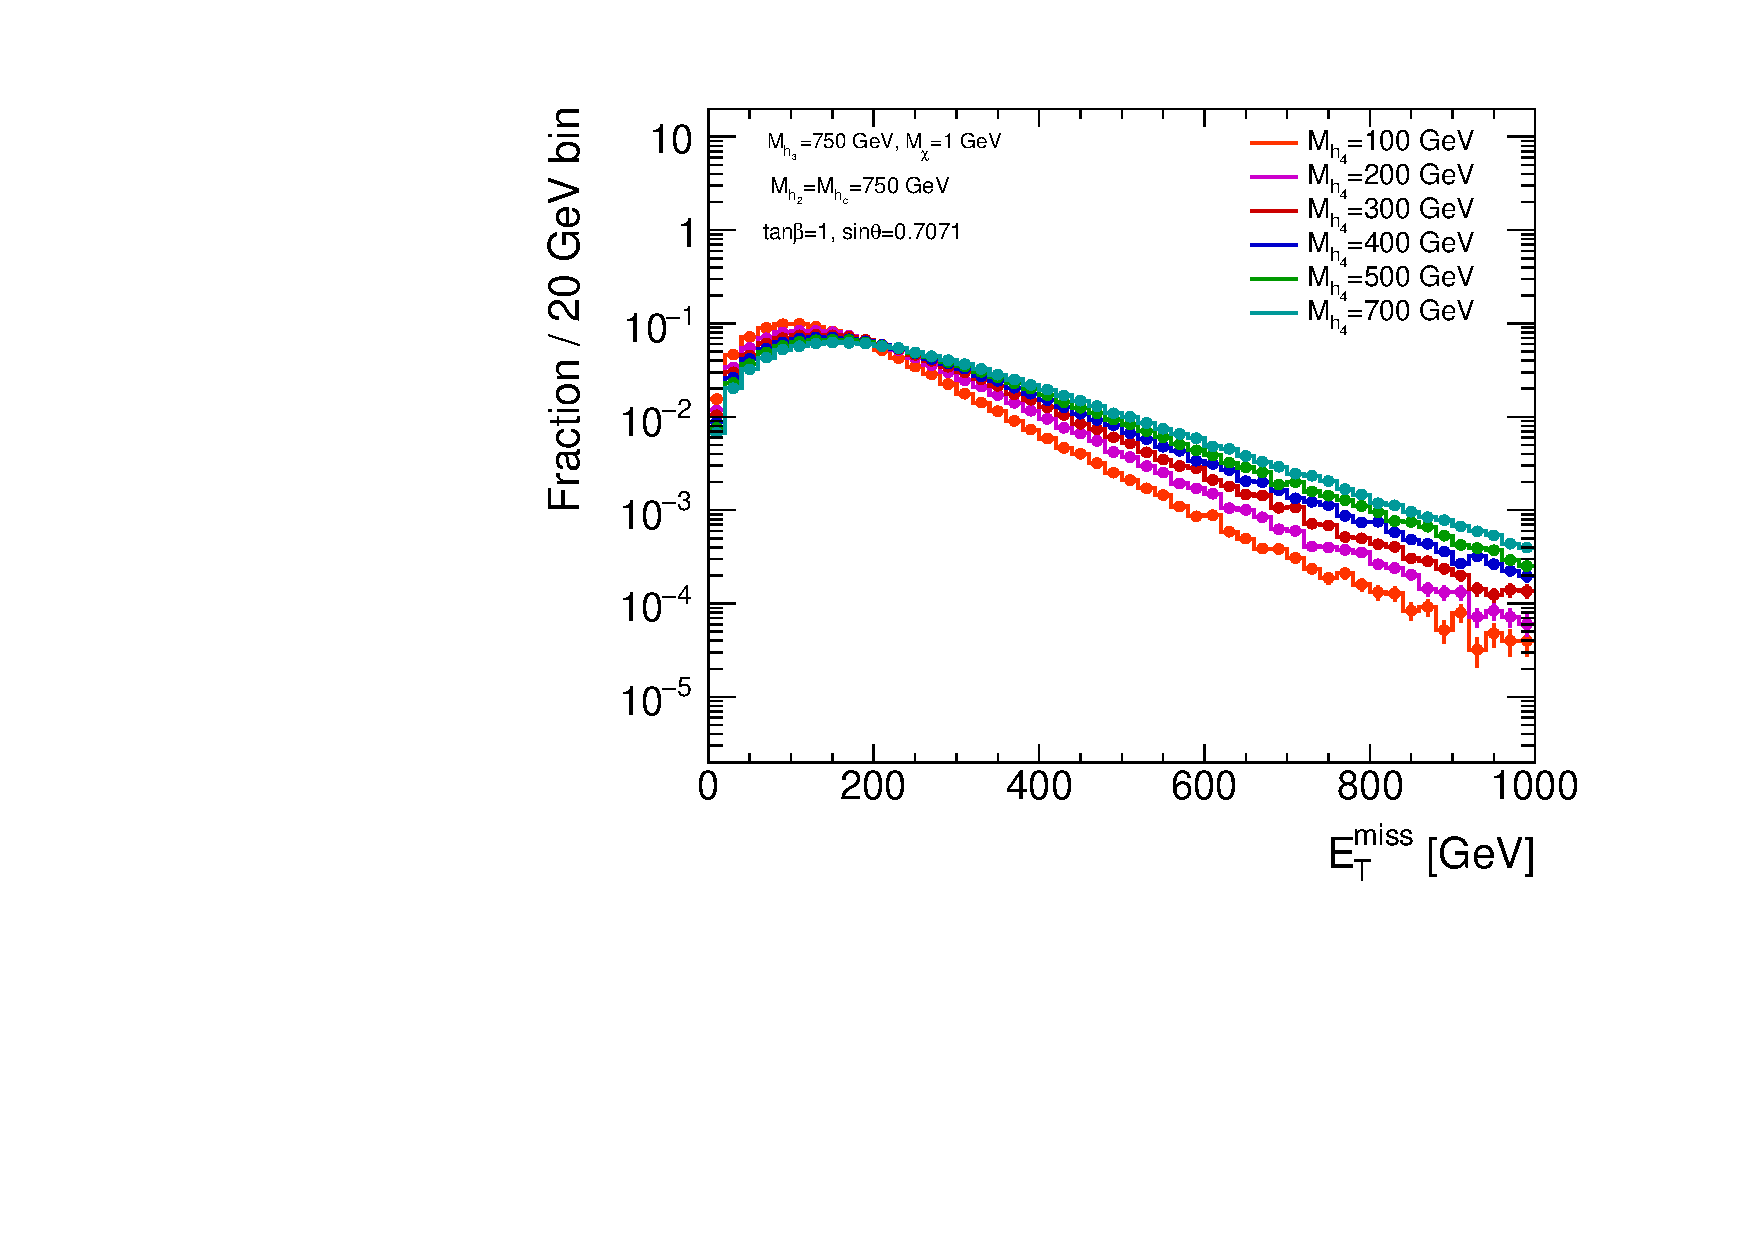
\includegraphics[width=\textwidth]{texinputs/04_grid/figures/DMHF/benchmarking/MDM_1_MA_750_sinp_0.7071_tanb_1.0_SCAN_Ma/metlog.pdf}
%    \caption{$E_{T}^{miss}$}
%  \end{subfigure}
%  \begin{subfigure}[b]{0.49\textwidth}
%    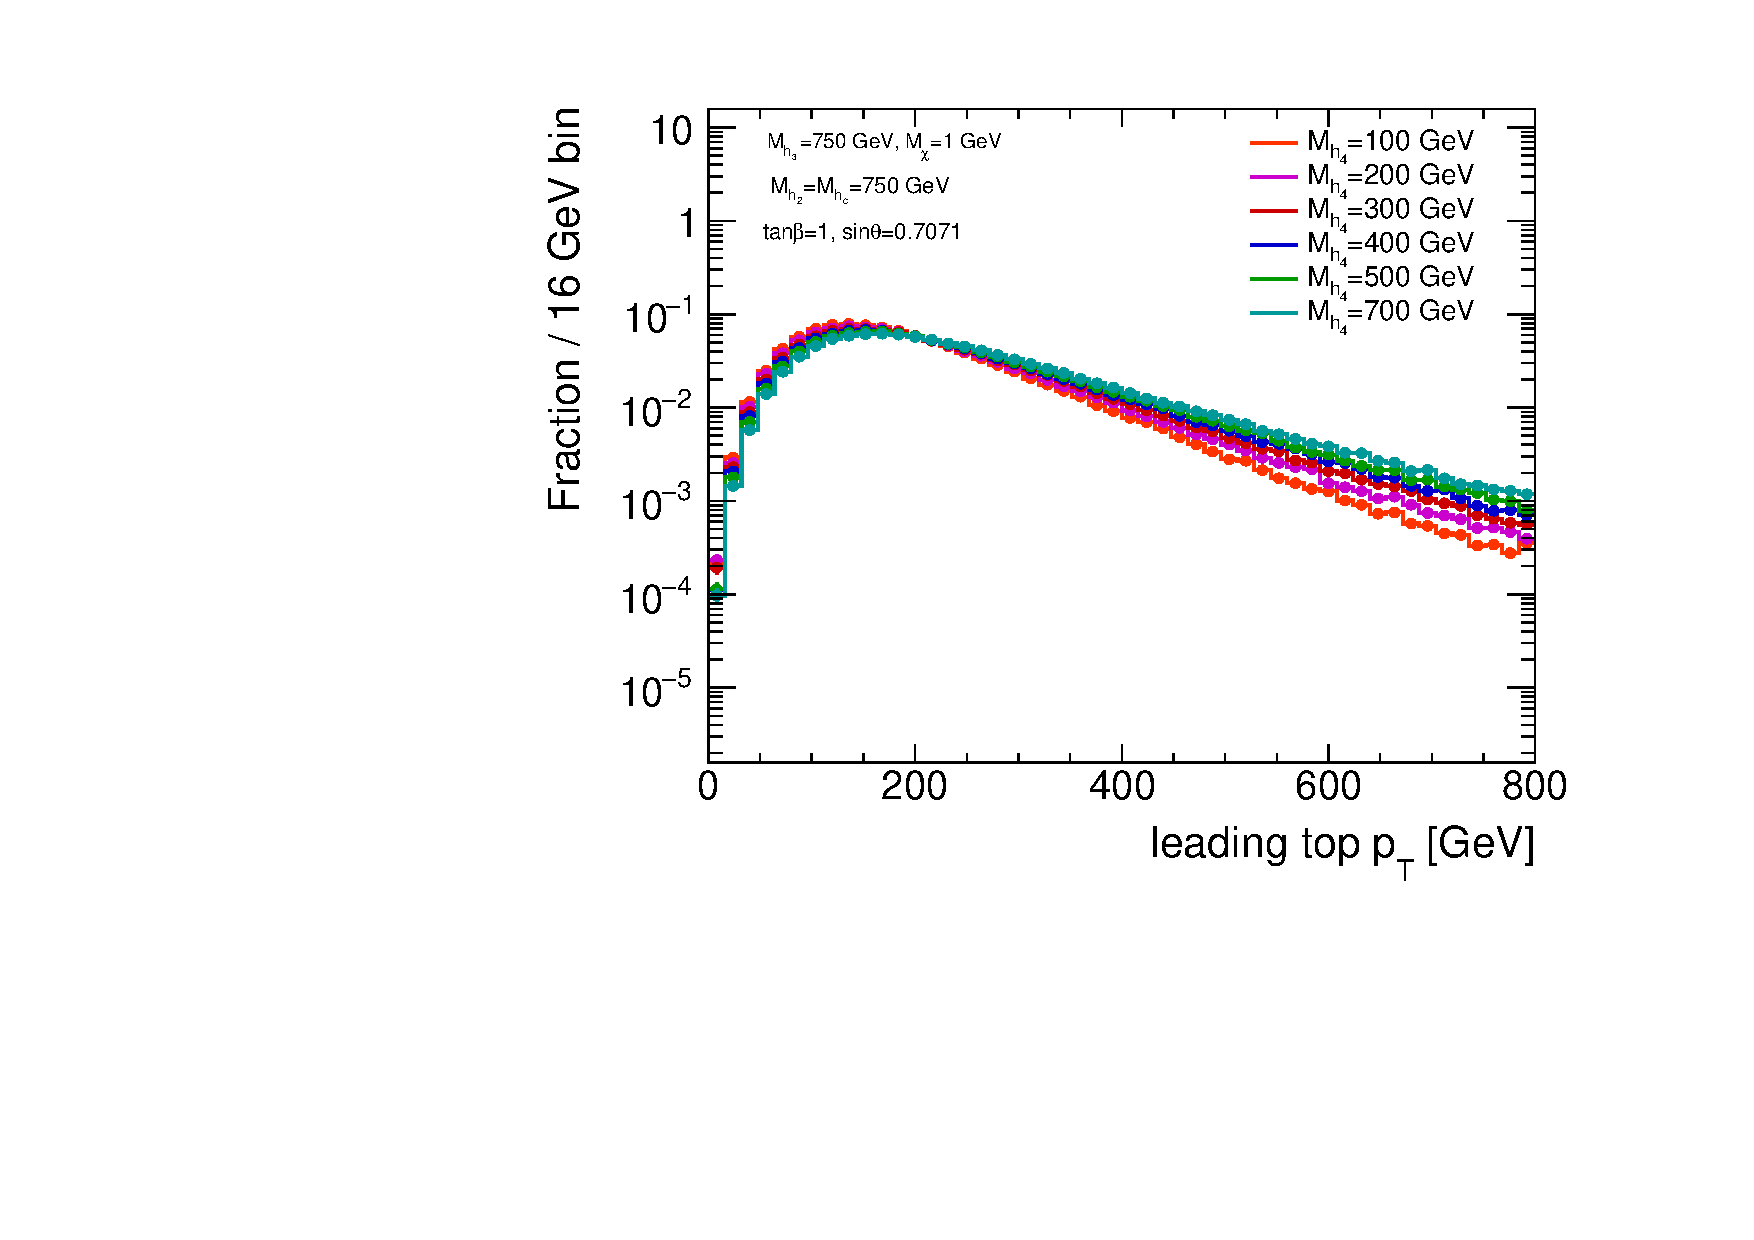
\includegraphics[width=\textwidth]{texinputs/04_grid/figures/DMHF/benchmarking/MDM_1_MA_750_sinp_0.7071_tanb_1.0_SCAN_Ma/top1ptlog.pdf}
%    \caption{Leading top $p_{T}$}
%  \end{subfigure} \\
%  \begin{subfigure}[b]{0.49\textwidth}
%    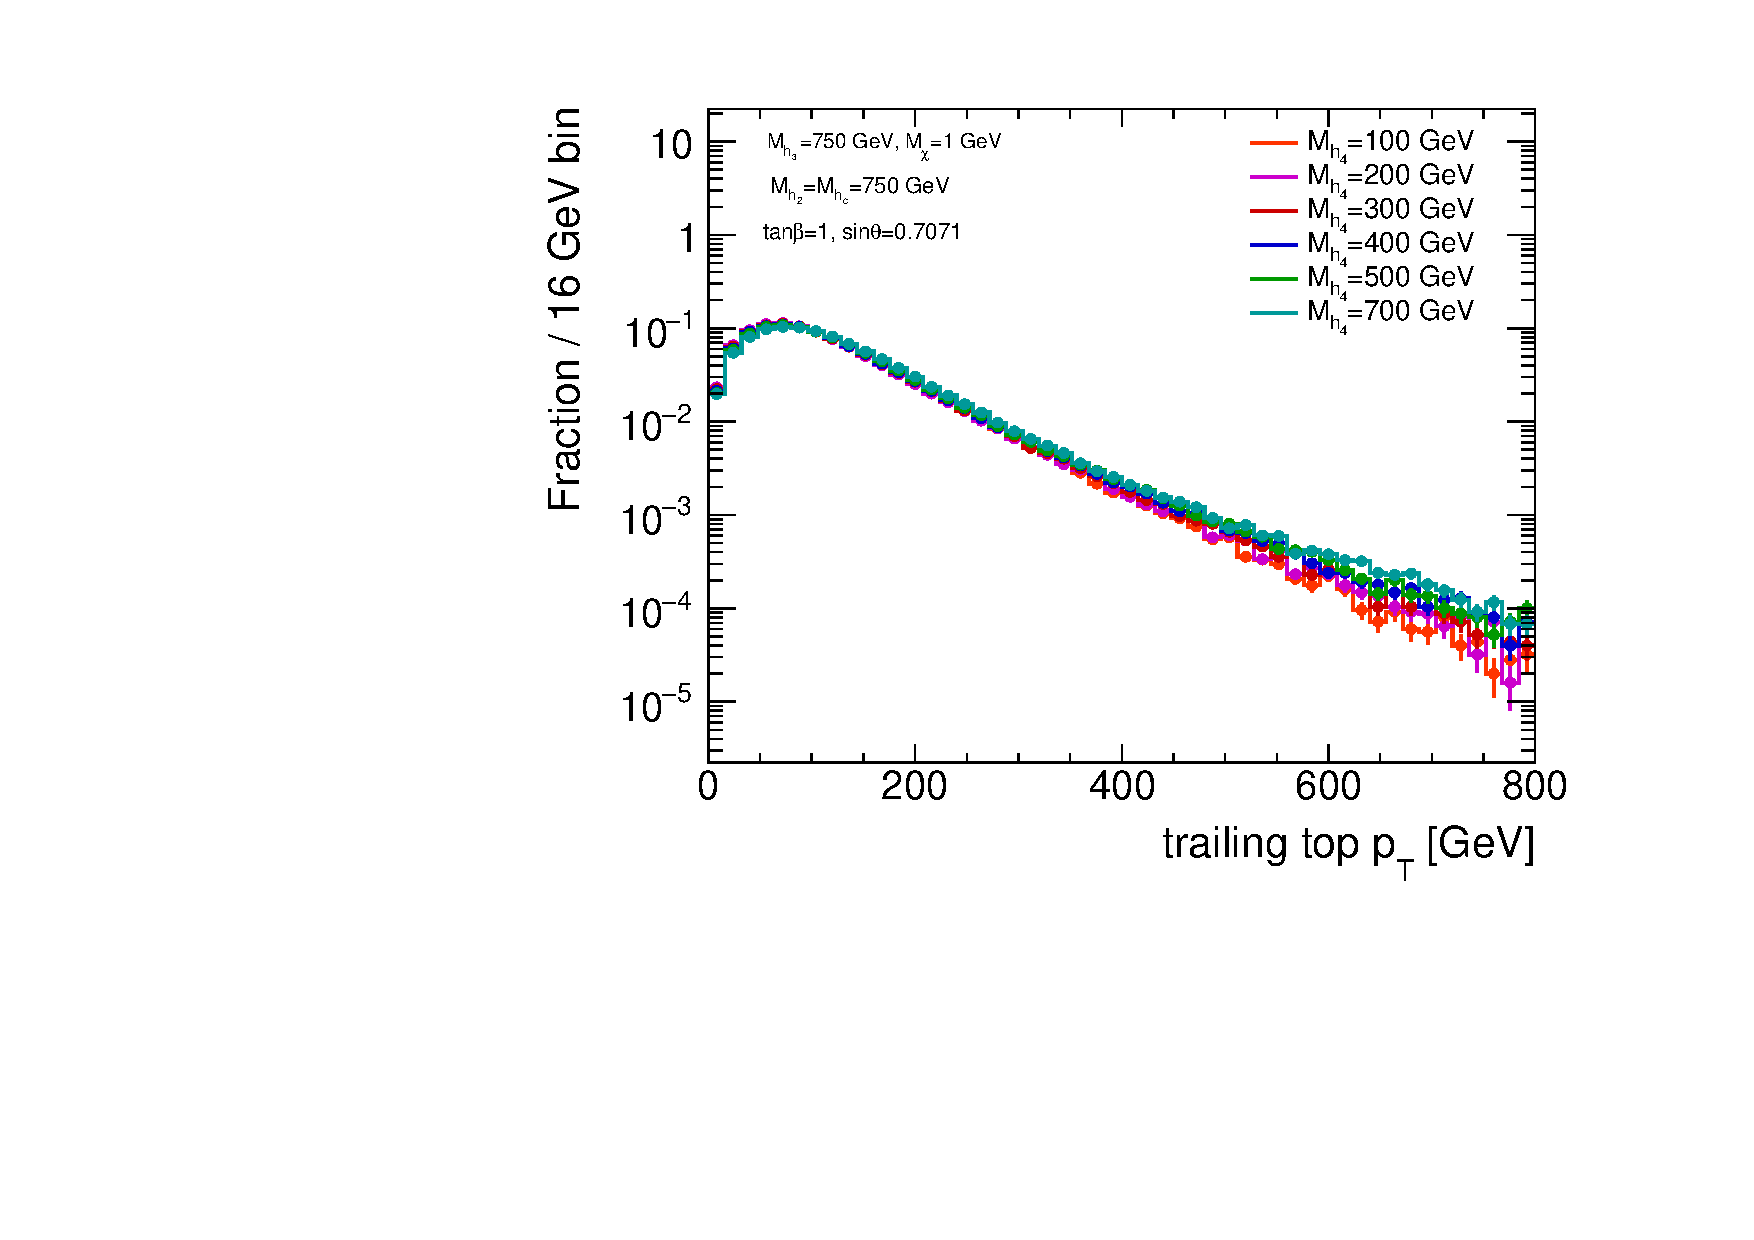
\includegraphics[width=\textwidth]{texinputs/04_grid/figures/DMHF/benchmarking/MDM_1_MA_750_sinp_0.7071_tanb_1.0_SCAN_Ma/top2ptlog.pdf}
%    \caption{Trailing top $p_{T}$}
%  \end{subfigure}
%  \caption{The $E_{T}^{miss}$, leading and trailing top $p_{T}$ distributions for inclusive $t\bar{t}+\chi\bar{\chi}$ production for various values of $\mathrm{M_a}$, with $\mathrm{M_A}=750$ GeV, $\mathrm{M_H}=\mathrm{M_{H^{\pm}}}=750$ GeV, $\tan\beta=1$, and $\sin\theta=0.7071$.}
%  \label{fig:kin_Ma}
%\end{figure}
%
%\begin{figure}
%  \centering
%  \begin{subfigure}[b]{0.49\textwidth}
%    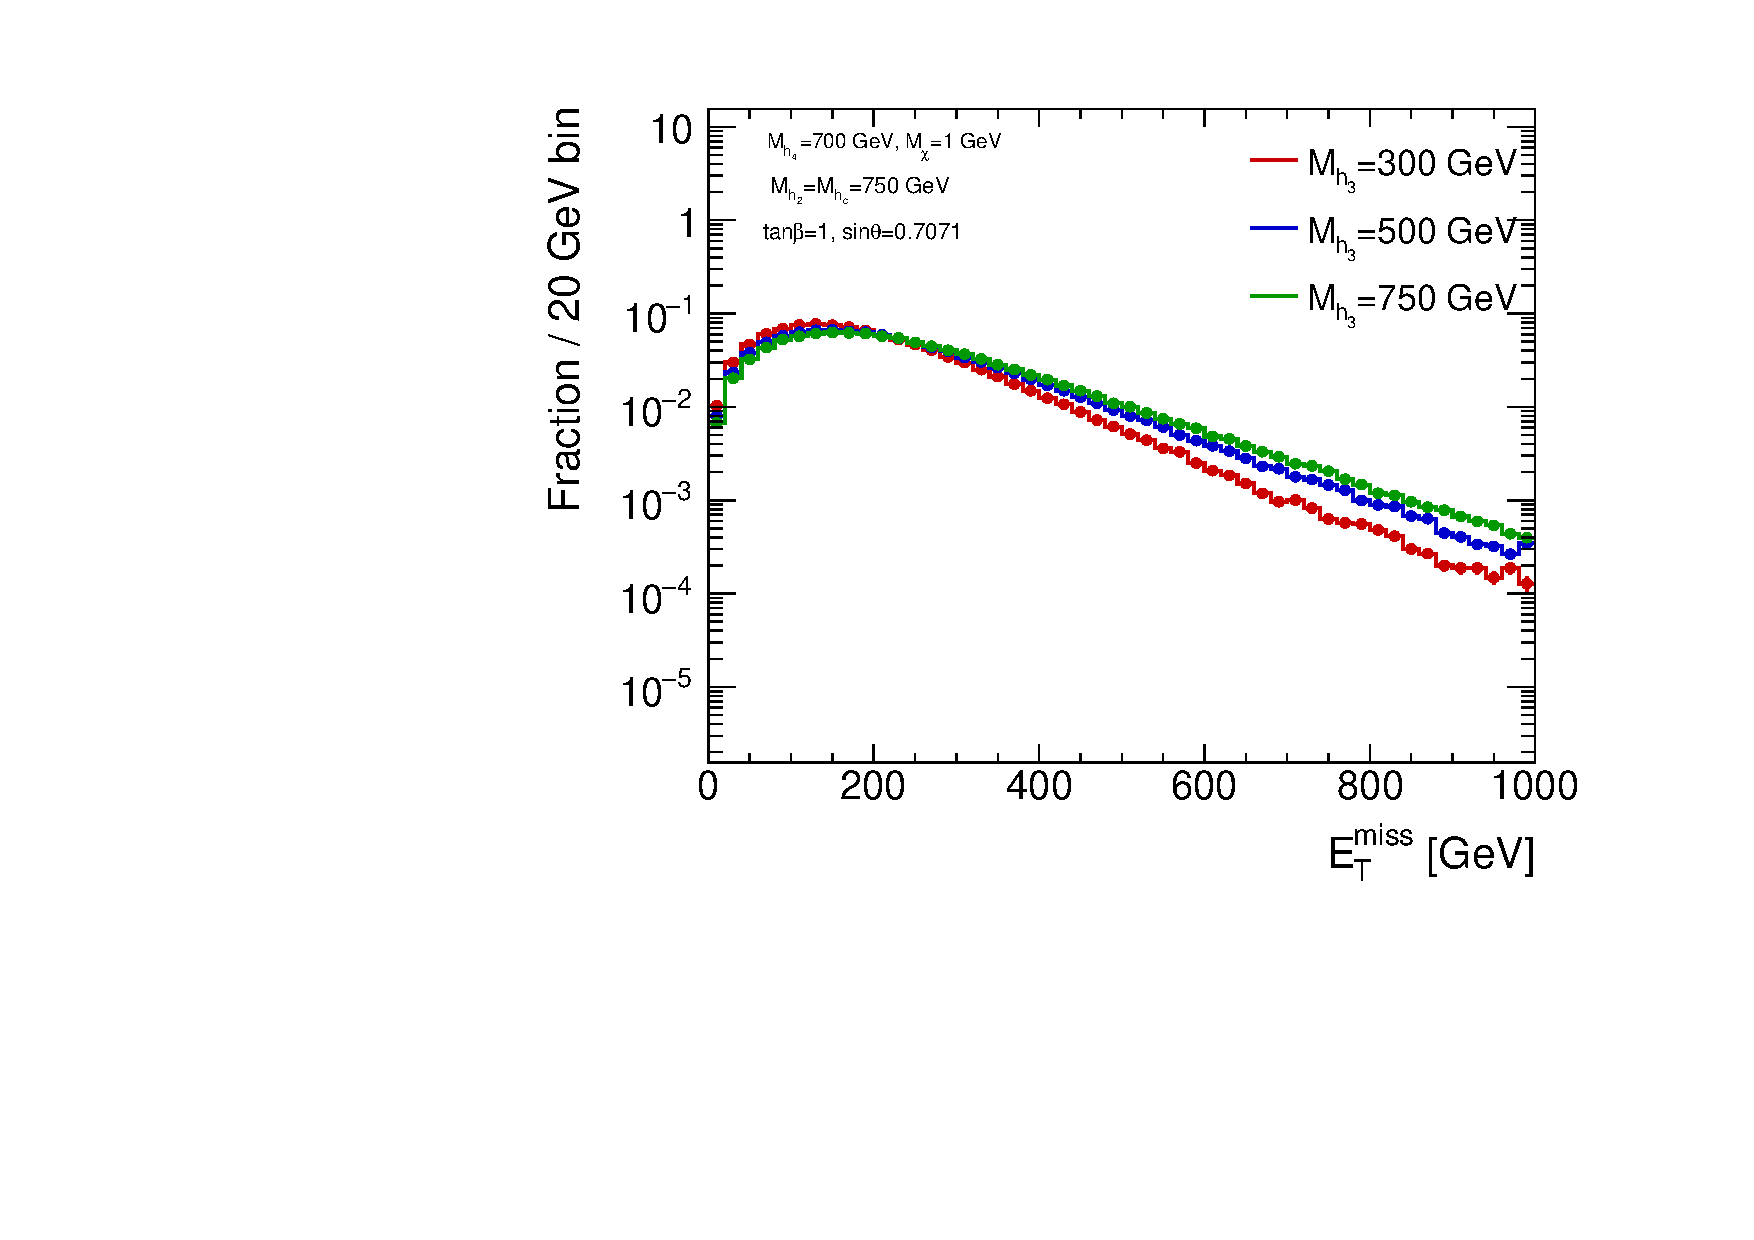
\includegraphics[width=\textwidth]{texinputs/04_grid/figures/DMHF/benchmarking/MDM_1_Ma_700_sinp_0.7071_tanb_1.0_SCAN_MA/metlog.pdf}
%    \caption{$E_{T}^{miss}$}
%  \end{subfigure}
%  \begin{subfigure}[b]{0.49\textwidth}
%    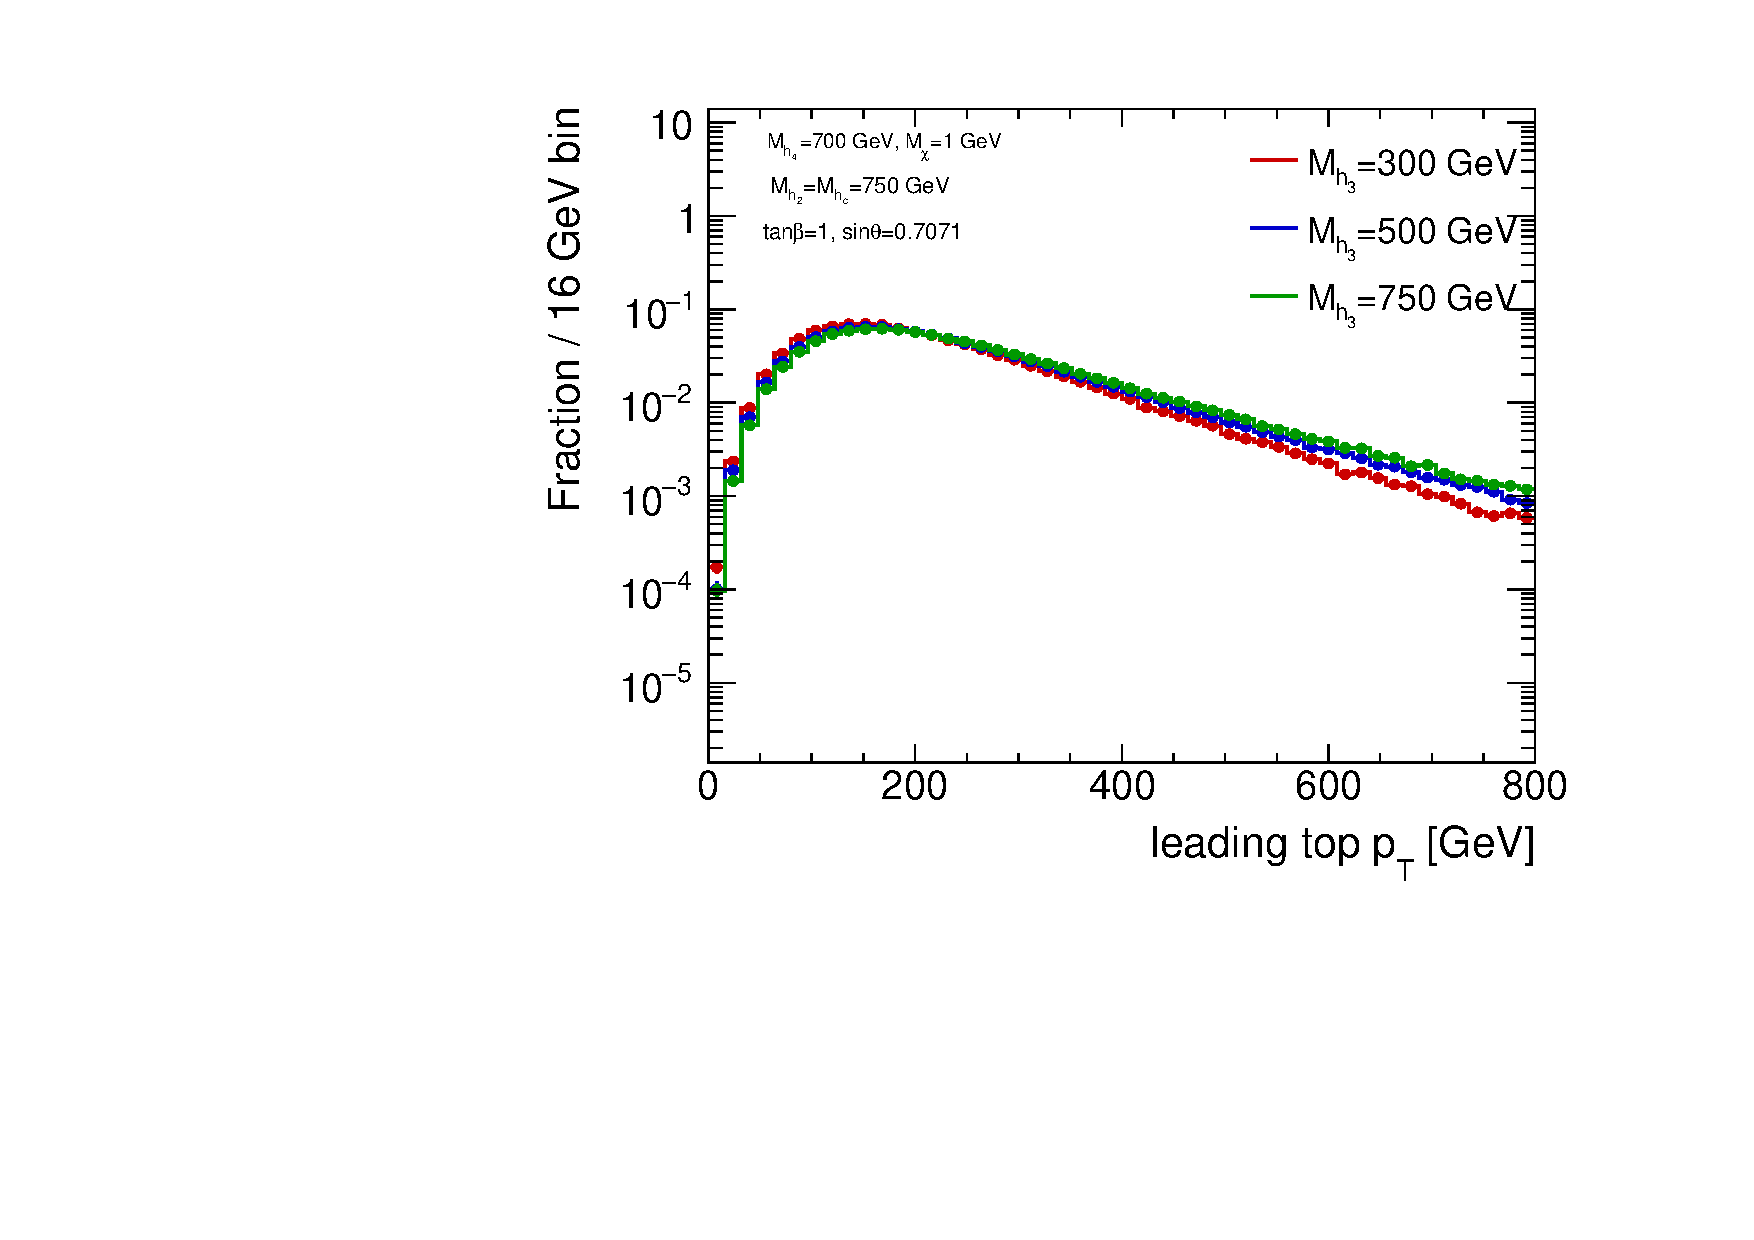
\includegraphics[width=\textwidth]{texinputs/04_grid/figures/DMHF/benchmarking/MDM_1_Ma_700_sinp_0.7071_tanb_1.0_SCAN_MA/top1ptlog.pdf}
%    \caption{Leading top $p_{T}$}
%  \end{subfigure} \\
%  \begin{subfigure}[b]{0.49\textwidth}
%    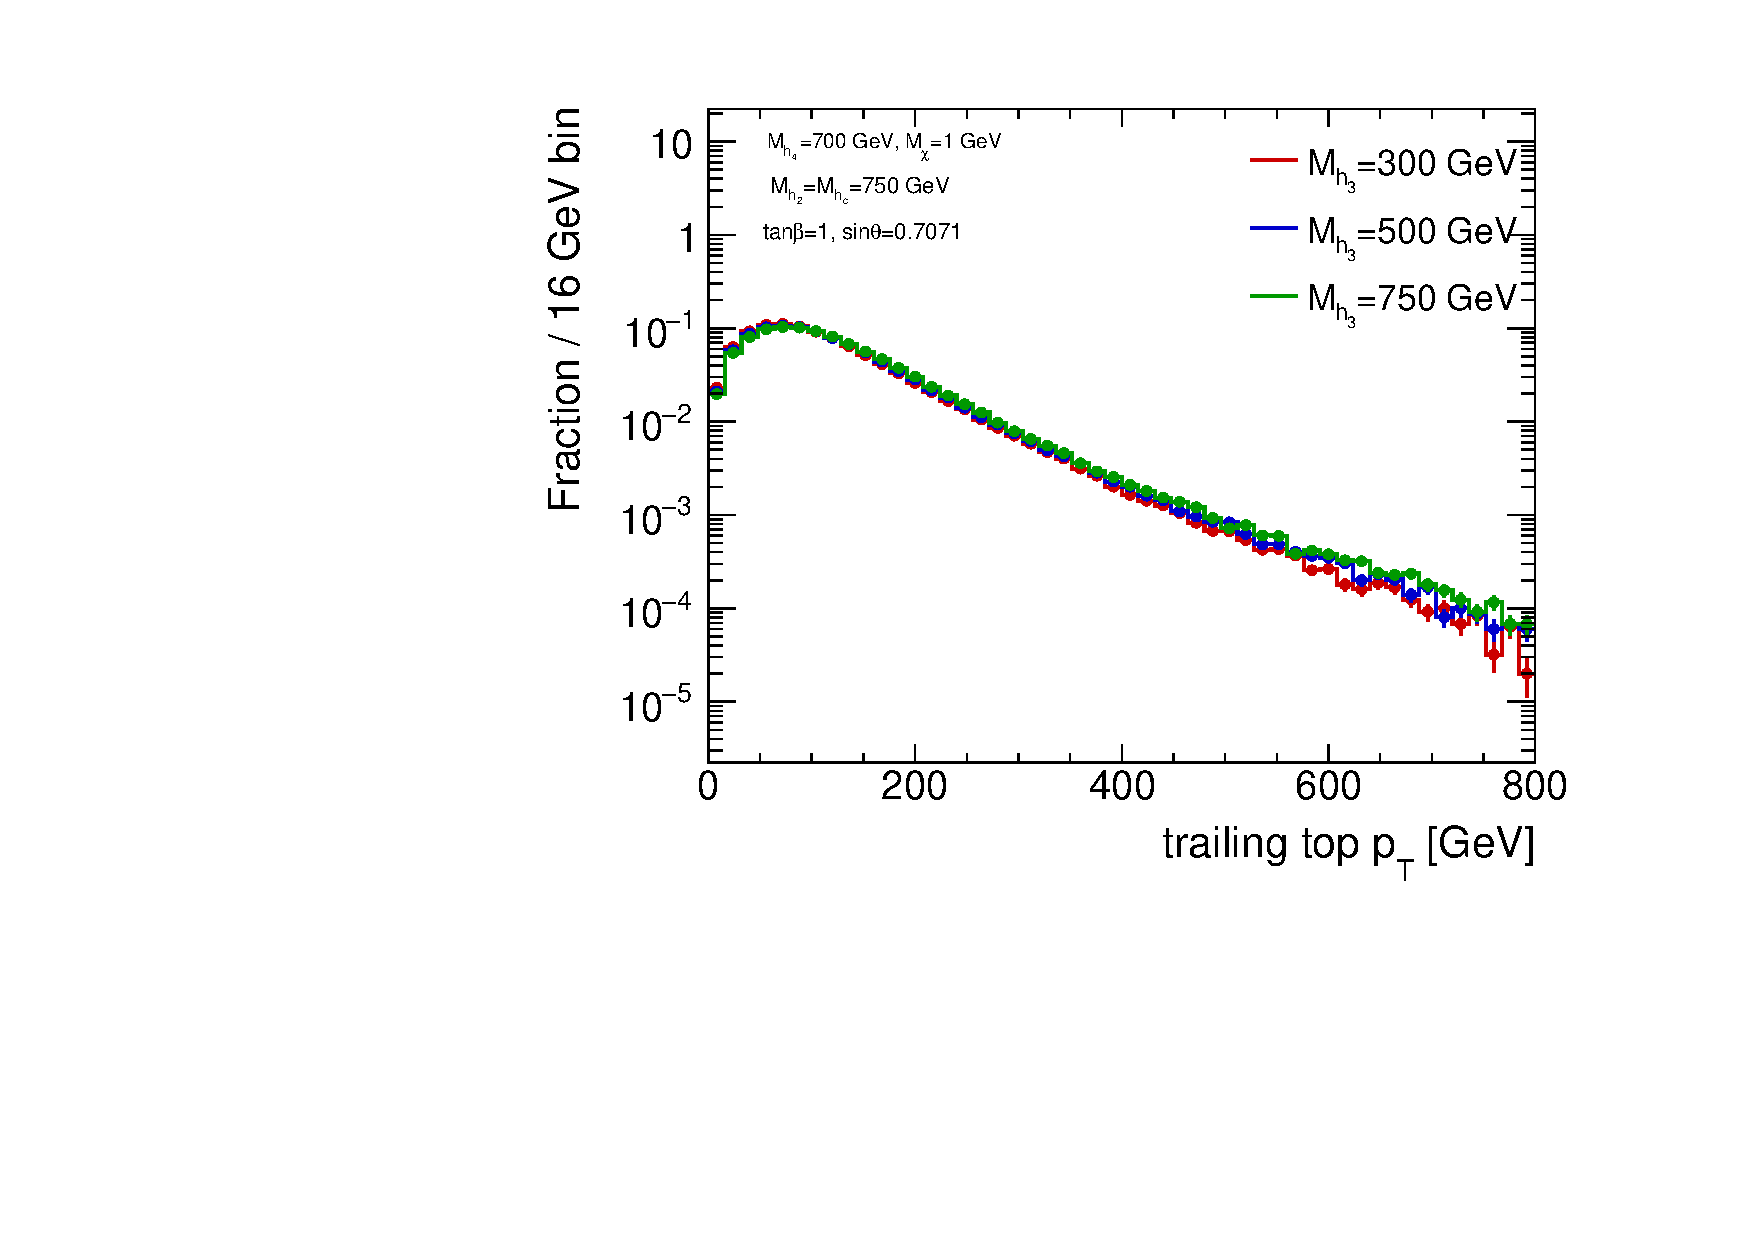
\includegraphics[width=\textwidth]{texinputs/04_grid/figures/DMHF/benchmarking/MDM_1_Ma_700_sinp_0.7071_tanb_1.0_SCAN_MA/top2ptlog.pdf}
%    \caption{Trailing top $p_{T}$}
%  \end{subfigure}
%  \caption{The $E_{T}^{miss}$, leading and trailing top $p_{T}$ distributions for inclusive $t\bar{t}+\chi\bar{\chi}$ production for various values of $\mathrm{M_A}$, with $\mathrm{M_a}=700$ GeV, $\mathrm{M_H}=\mathrm{M_{H^{\pm}}}=750$ GeV, $\tan\beta=1$, and $\sin\theta=0.7071$.}
%  \label{fig:kin_MA}
%\end{figure}
%%%%%-----------------------------------------------------------------------------------------
%\subsubsection{Comparison with DMsimp Pseudoscalar Model}
%
%To date, simplified models of DM (\texttt{DMsimp}) are used to interpret Run II CMS and ATLAS HF+DM searches. A comparison of the pertinent kinematic distributions between the pseudoscalar simplified model and the 2HDM+a model for the same value of $\mathrm{M_{a}}$ are shown in Fig.~\ref{kin_DMSimpV2HDMa}. The kinematics of the pseudoscalar \texttt{DMsimp} model with $\mathrm{M_{a}}=100$ GeV map directly onto those of the 2HDM+a model with $\mathrm{M_{a}}=100$ GeV, $\mathrm{M_{A}}=600$ GeV, $\mathrm{M_{H}}=\mathrm{M_{H^{\pm}}}=600$ GeV, $\sin\theta=0.7071$, and $\tan\beta=1$. From the mass distribution of the $\chi\bar{\chi}$ shown in Fig.~\ref{fig:mchichi_DMsimpV2HDMa}, it is evident that the 2HDM+a model contains contributions from both the light and heavy pseudoscalar mediator as in the \texttt{DMsimp} model.
%
%\begin{figure}
%  \centering
%  \begin{subfigure}[b]{0.49\textwidth}
%    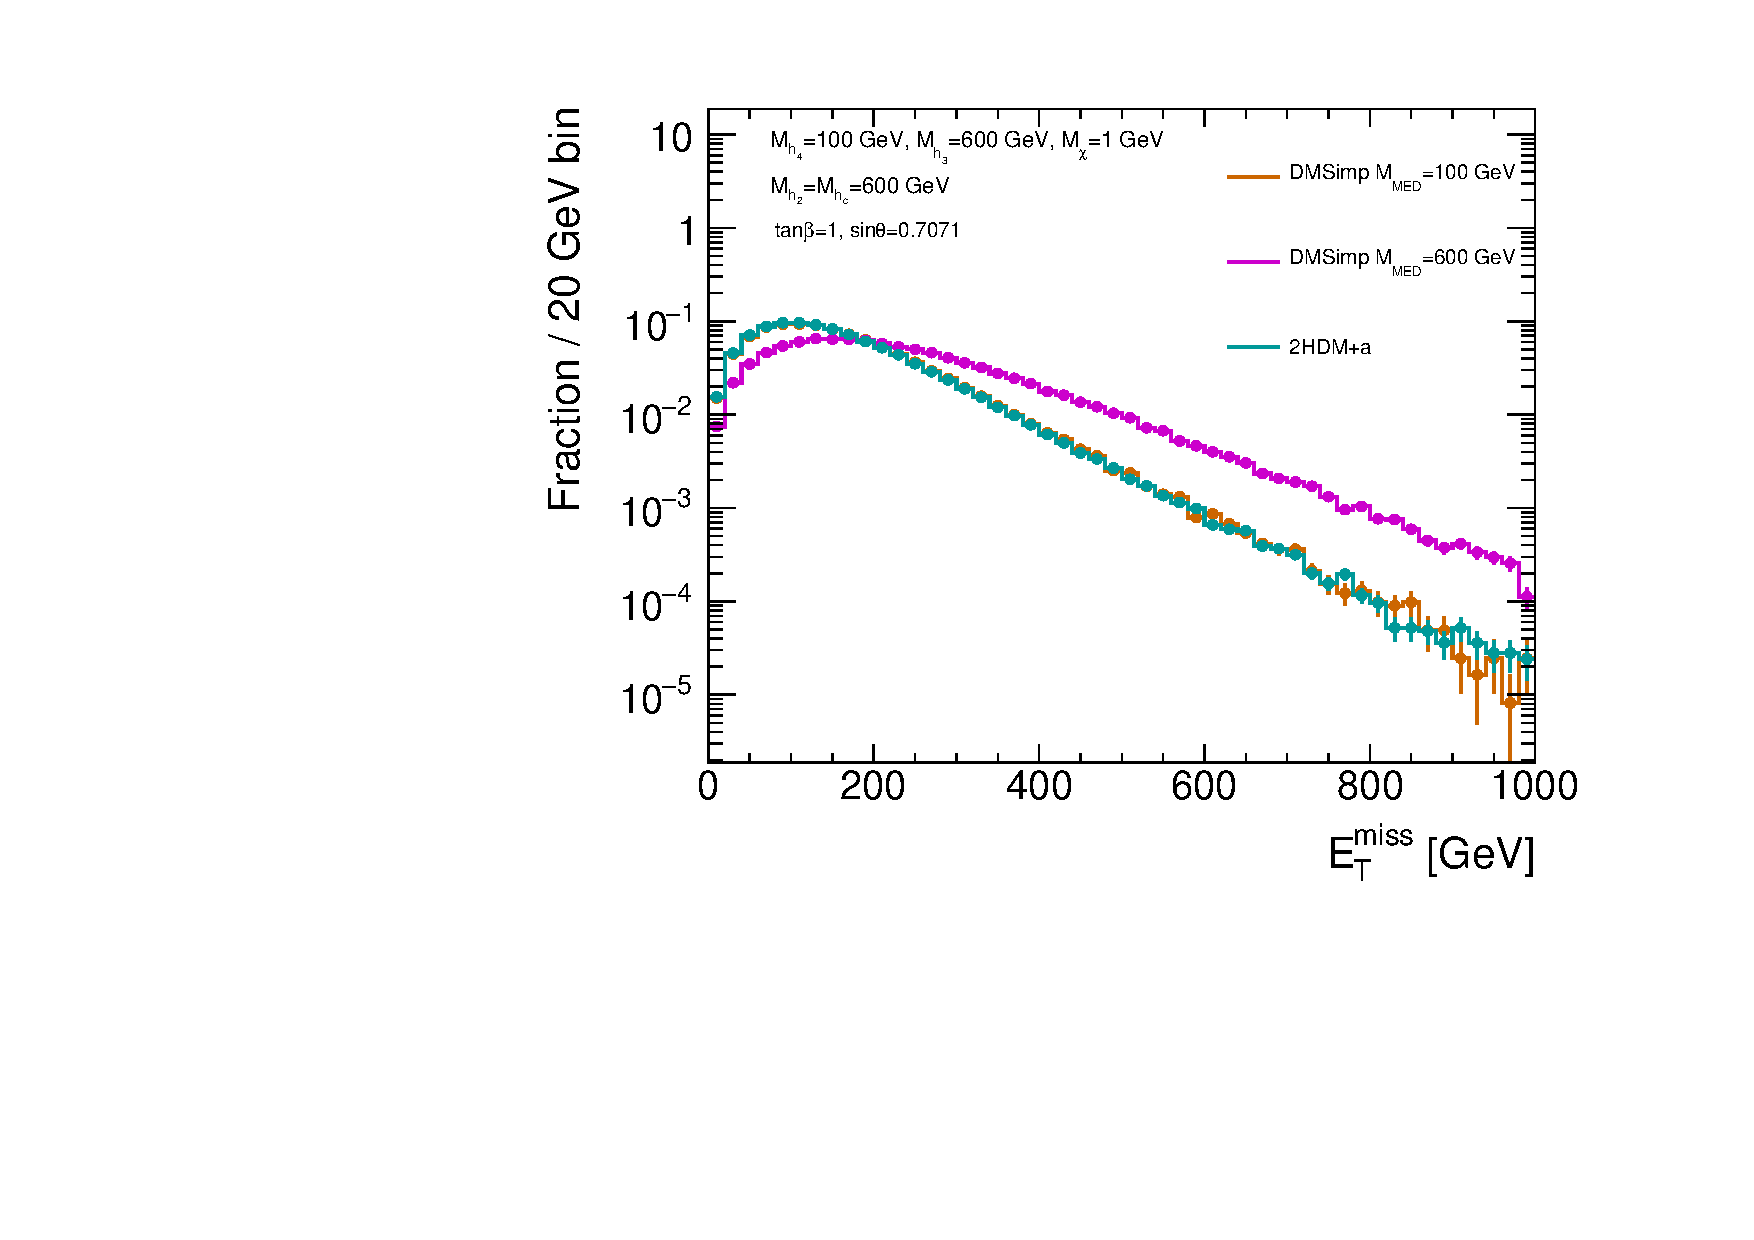
\includegraphics[width=\textwidth]{texinputs/04_grid/figures/DMHF/benchmarking/MDM_1_Ma_100_MA_600_sinp_0.7071_tanb_1.0_VS_DMSimp_100_600_Decayed/metlog.pdf}
%    \caption{$E_{T}^{miss}$}
%  \end{subfigure}
%  \begin{subfigure}[b]{0.49\textwidth}
%    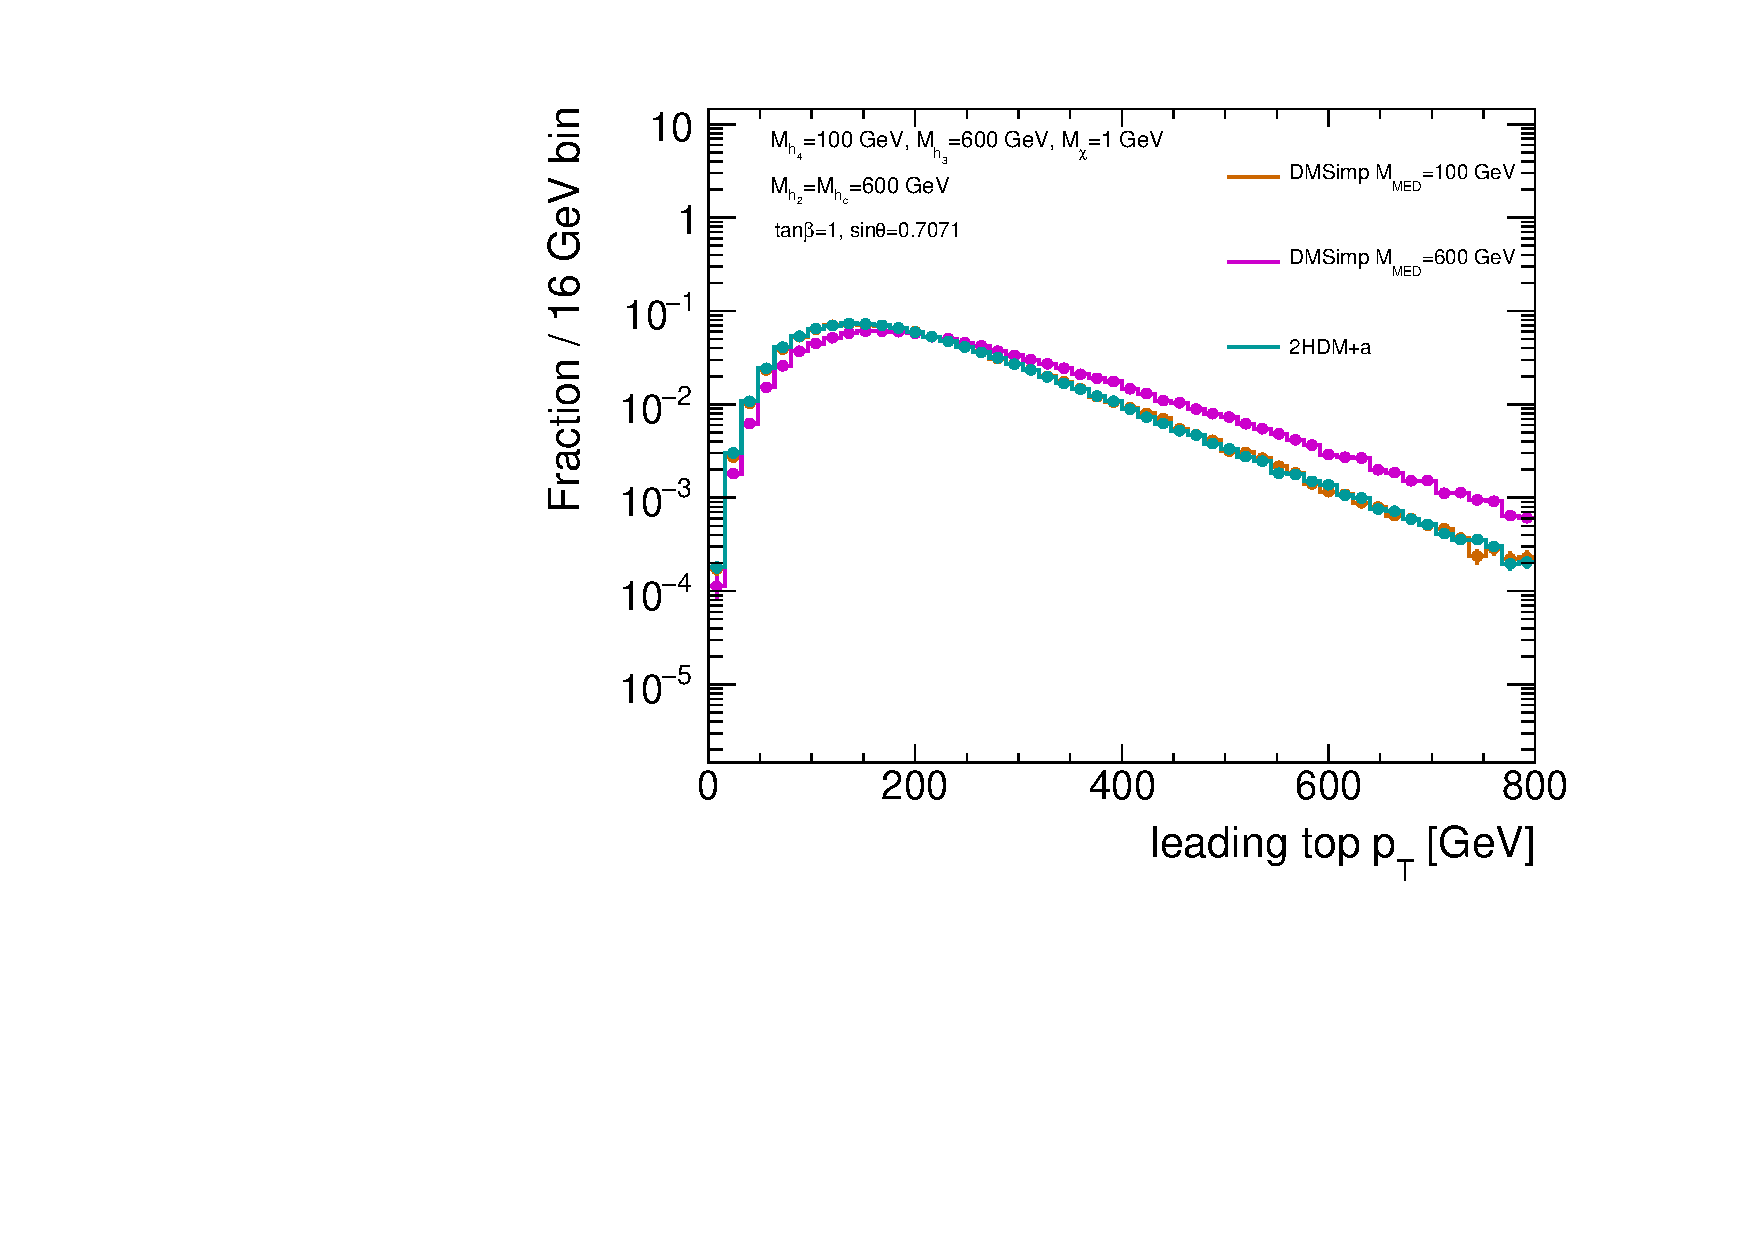
\includegraphics[width=\textwidth]{texinputs/04_grid/figures/DMHF/benchmarking/MDM_1_Ma_100_MA_600_sinp_0.7071_tanb_1.0_VS_DMSimp_100_600_Decayed/top1ptlog.pdf}
%    \caption{Leading top $p_{T}$}
%  \end{subfigure} \\
%  \begin{subfigure}[b]{0.49\textwidth}
%    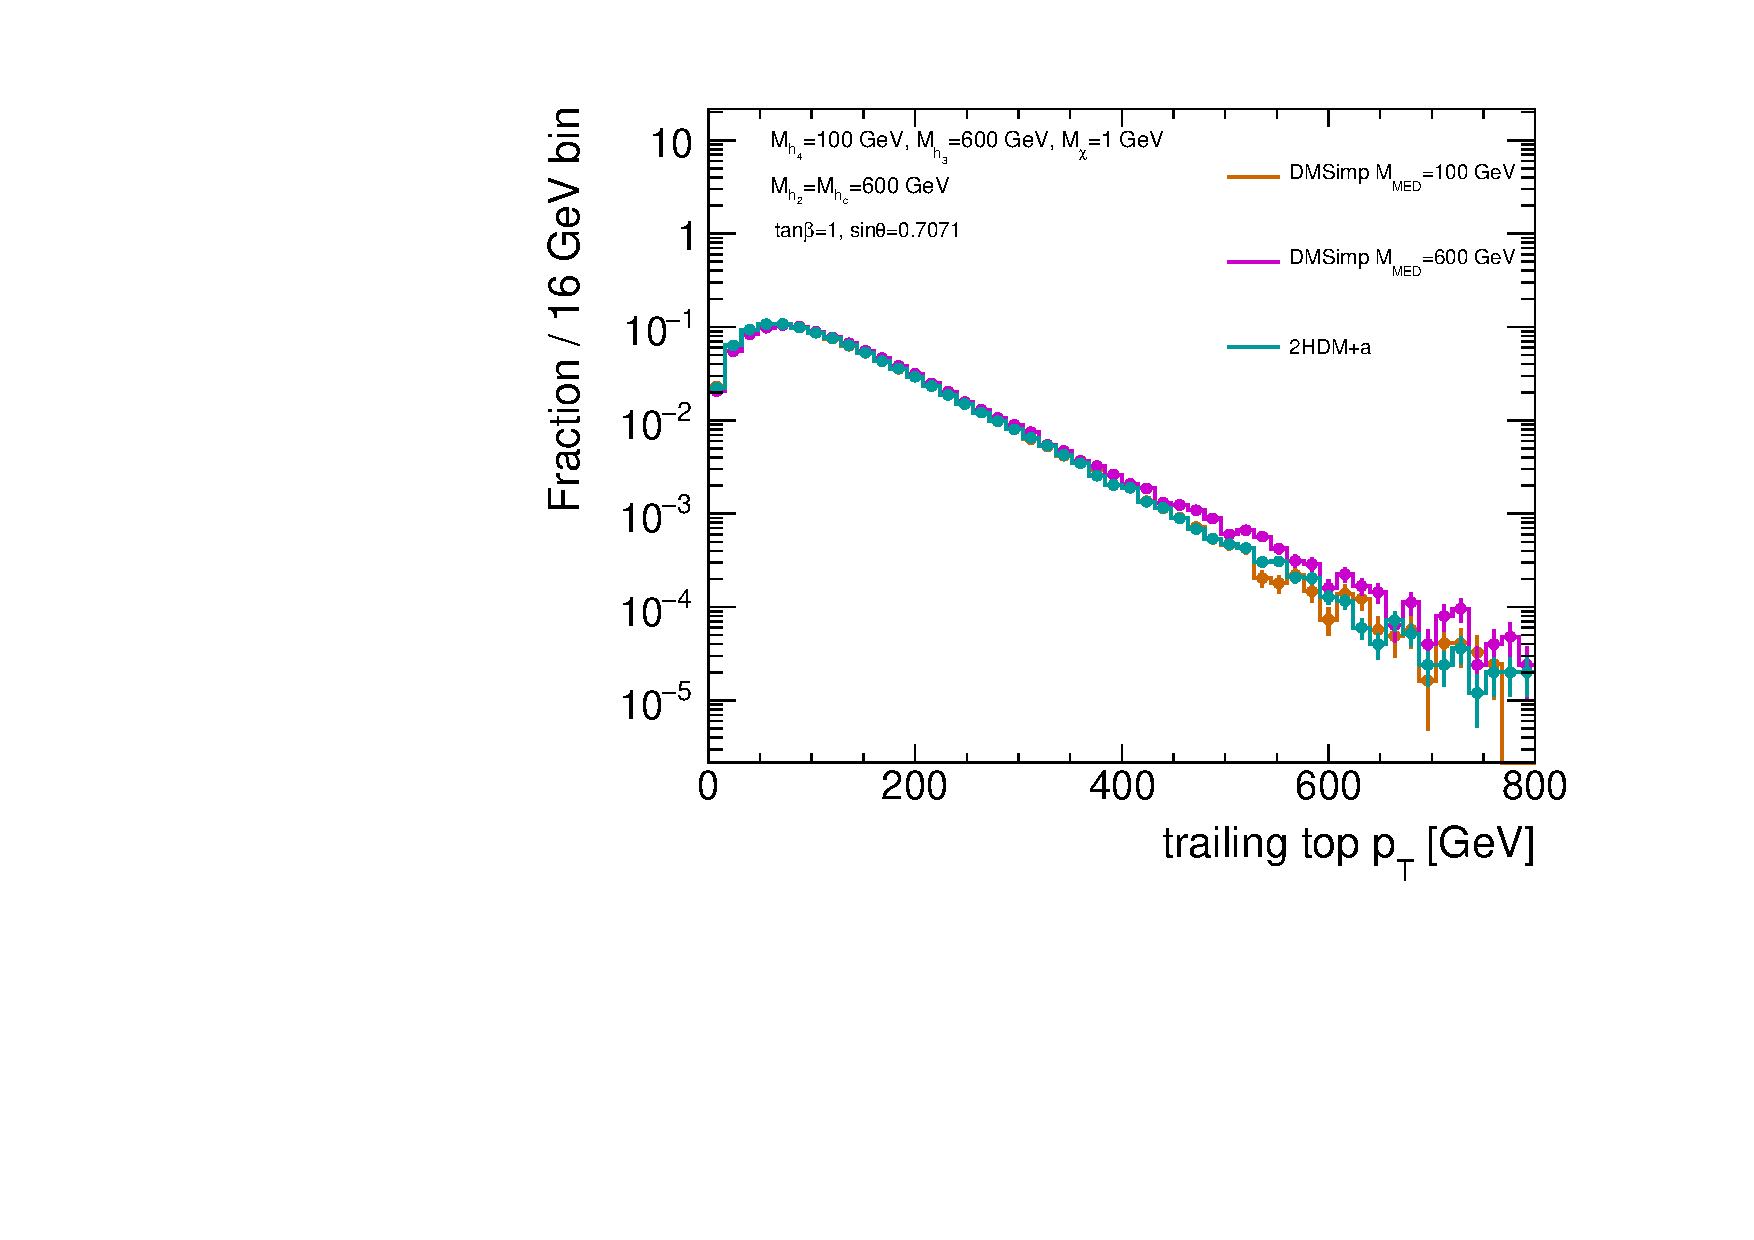
\includegraphics[width=\textwidth]{texinputs/04_grid/figures/DMHF/benchmarking/MDM_1_Ma_100_MA_600_sinp_0.7071_tanb_1.0_VS_DMSimp_100_600_Decayed/top2ptlog.pdf}
%    \caption{Trailing top $p_{T}$}
%  \end{subfigure}
%  \caption{The $E_{T}^{miss}$, leading and trailing top $p_{T}$ distributions for inclusive $t\bar{t}+\chi\bar{\chi}$ production for various values of $\mathrm{M_A}$, with $\mathrm{M_a}=700$ GeV, $\mathrm{M_H}=\mathrm{M_{H^{\pm}}}=750$ GeV, $\tan\beta=1$, and $\sin\theta=0.7071$.}
%  \label{fig:kin_DMSimpV2HDMa}
%\end{figure}
%
%\begin{figure}
%  \centering
%  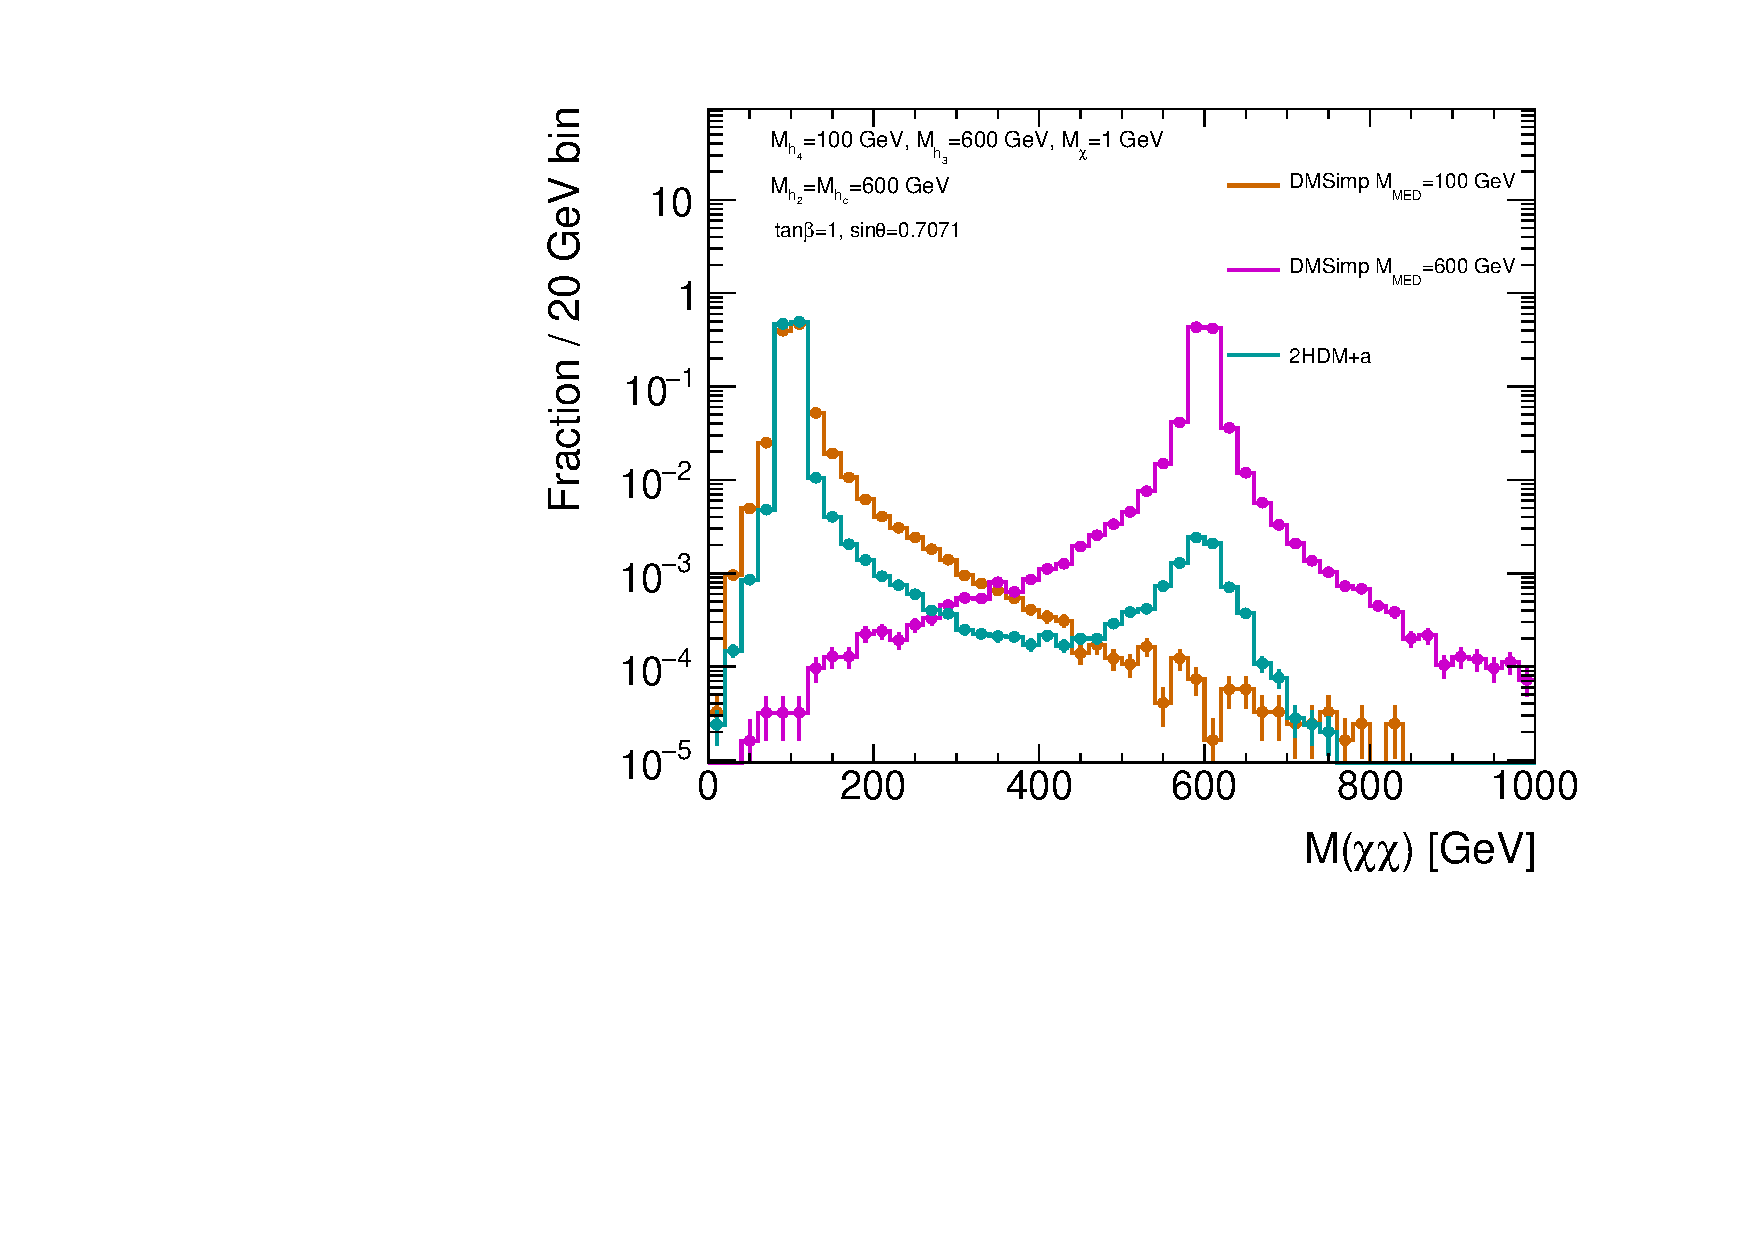
\includegraphics[width=0.6\textwidth]{texinputs/04_grid/figures/DMHF/benchmarking/MDM_1_Ma_100_MA_600_sinp_0.7071_tanb_1.0_VS_DMSimp_100_600_Decayed/mchichi.pdf}
%  \caption{The mass distribution of the $\chi\bar{\chi}$ system for \texttt{DMsimp} pseudoscalar models with $\mathrm{M_a}=100$ GeV and $\mathrm{M_a}=600$ GeV, compared with 2HDM+a with $\mathrm{M_a}=100$ GeV, $\mathrm{M_A}=600$ GeV, $\mathrm{M_H}=\mathrm{M_{H^{\pm}}}=600$ GeV, $\sin\theta=0.7071$ and $\tan\beta=1$.}
%  \label{fig:mchichi_DMsimpV2HDMa}
%\end{figure}
%
%In Fig.~\ref{fig:DMSimpV2HDMa}, relevant kinematic distributions, commonly employed in HF+DM searches, are mapped from the \texttt{DMsimp} pseudoscalar models to the 2HDM+a model, with the mediator masses corresponding to the additional light pseudoscalar in the latter model. The dashed distributions represent the \texttt{DMsimp} model, while the solid are the 2HDM+a model distributions. The $t\bar{t}+\chi\bar{\chi}$ process was generated at LO precision using both models. As can be seen, the kinematics do not change appreciably between the models generated at the same value of $\mathrm{M_{a}}$. A discussion on cross-section rescaling procedures can be found in the following section.
%
%\begin{figure}
%  \centering    
%  \begin{subfigure}[b]{0.49\textwidth}
%    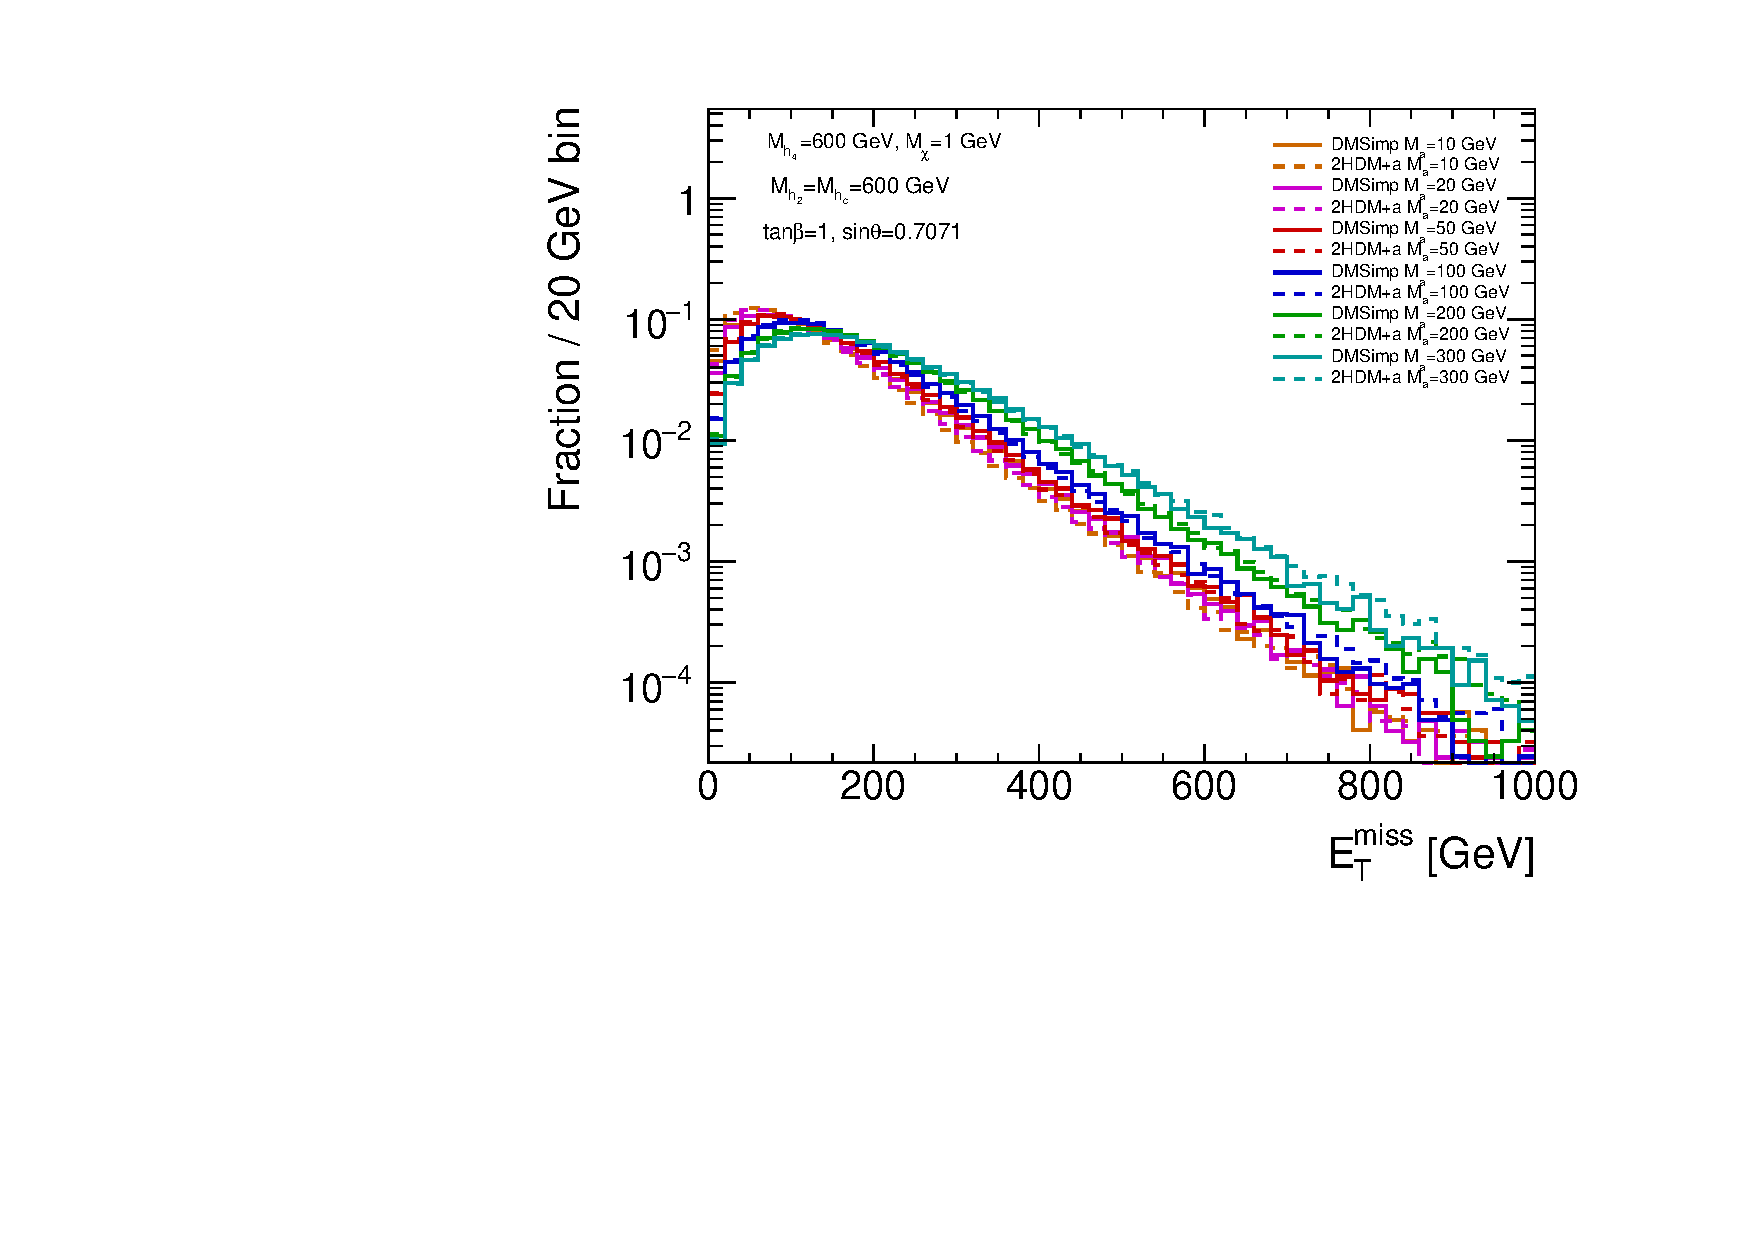
\includegraphics[width=\textwidth]{texinputs/04_grid/figures/DMHF/benchmarking/MDM_1_MA_600_sinp_0.7071_tanb_1.0_DMsimpV2HDMa/metlog.pdf}
%    \caption{$E_{T}^{miss}$}
%  \end{subfigure}
%  \begin{subfigure}[b]{0.49\textwidth}
%    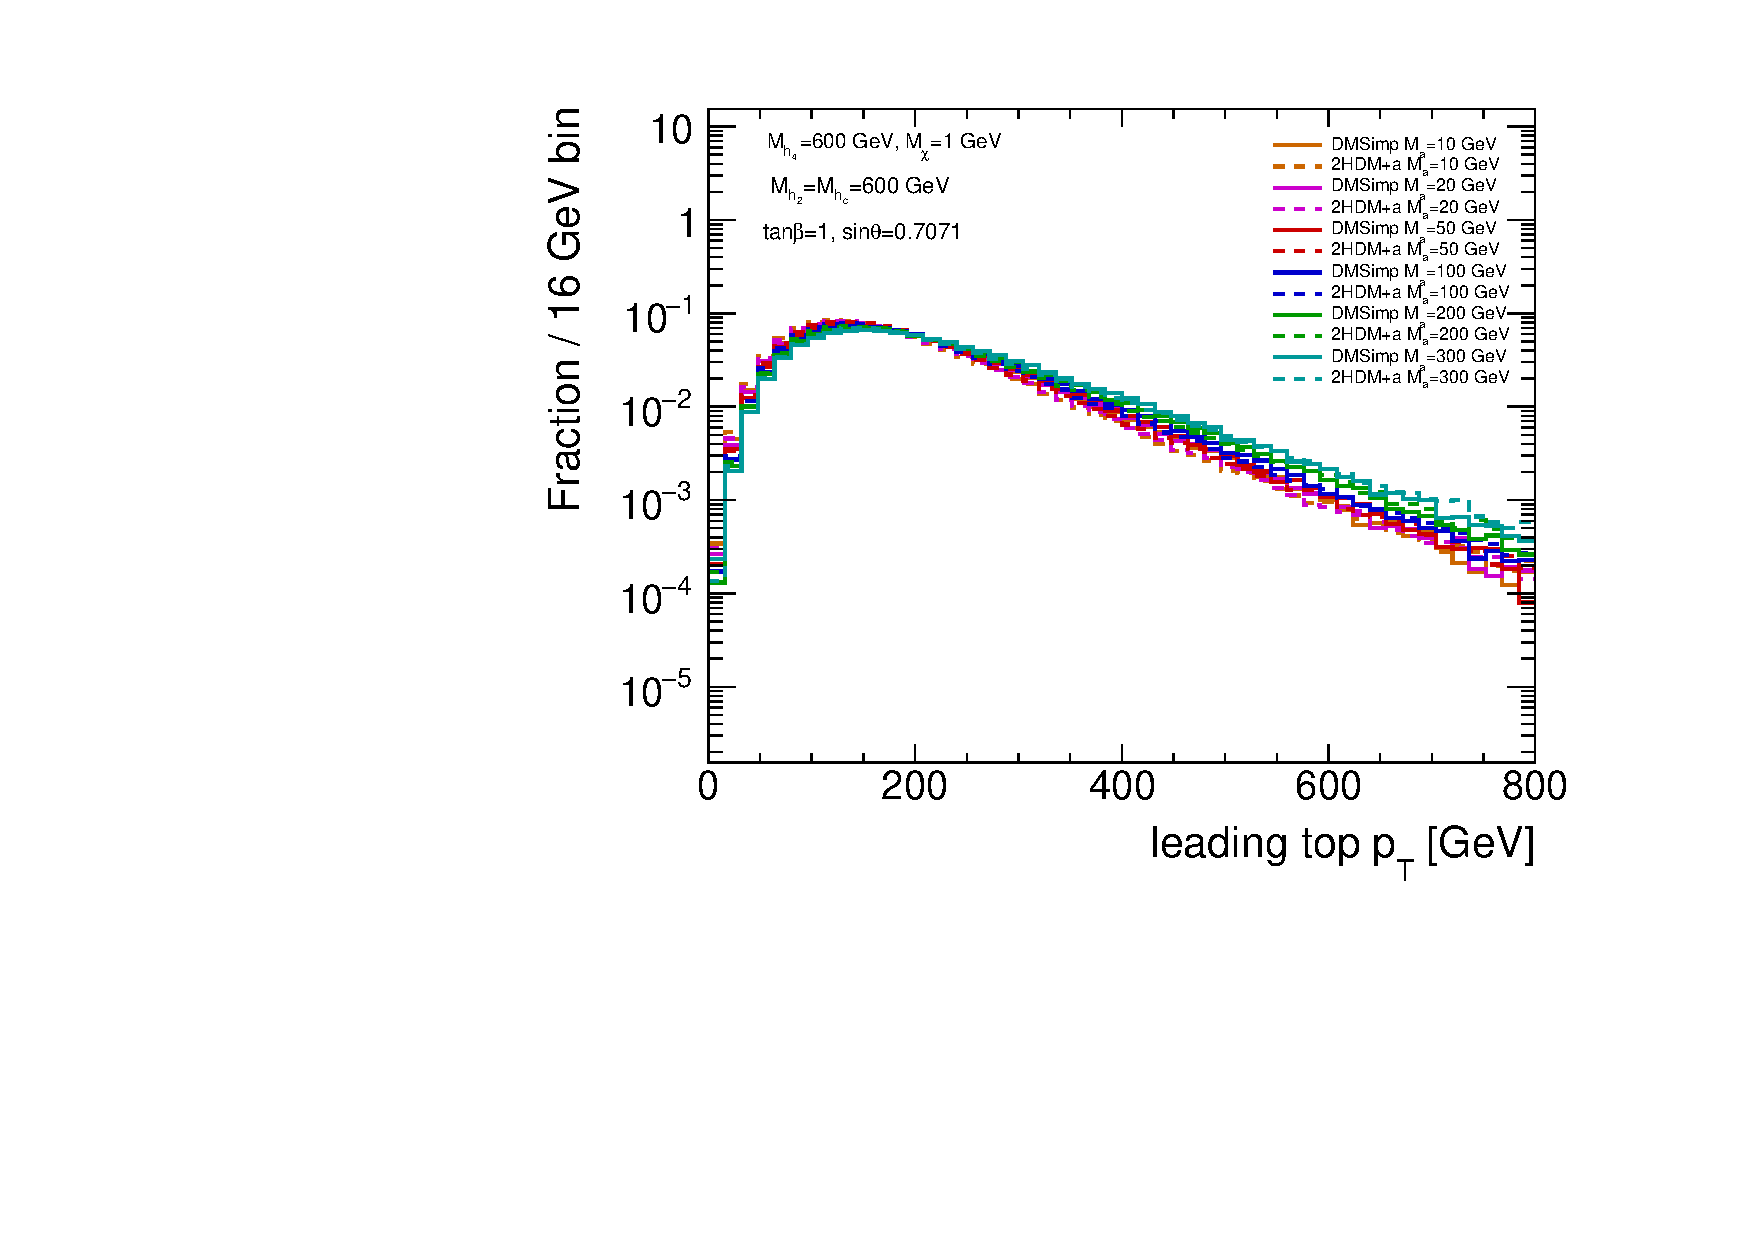
\includegraphics[width=\textwidth]{texinputs/04_grid/figures/DMHF/benchmarking/MDM_1_MA_600_sinp_0.7071_tanb_1.0_DMsimpV2HDMa/top1ptlog.pdf}
%    \caption{Leading top $p_{T}$}
%  \end{subfigure} \\
%  \begin{subfigure}[b]{0.49\textwidth}
%    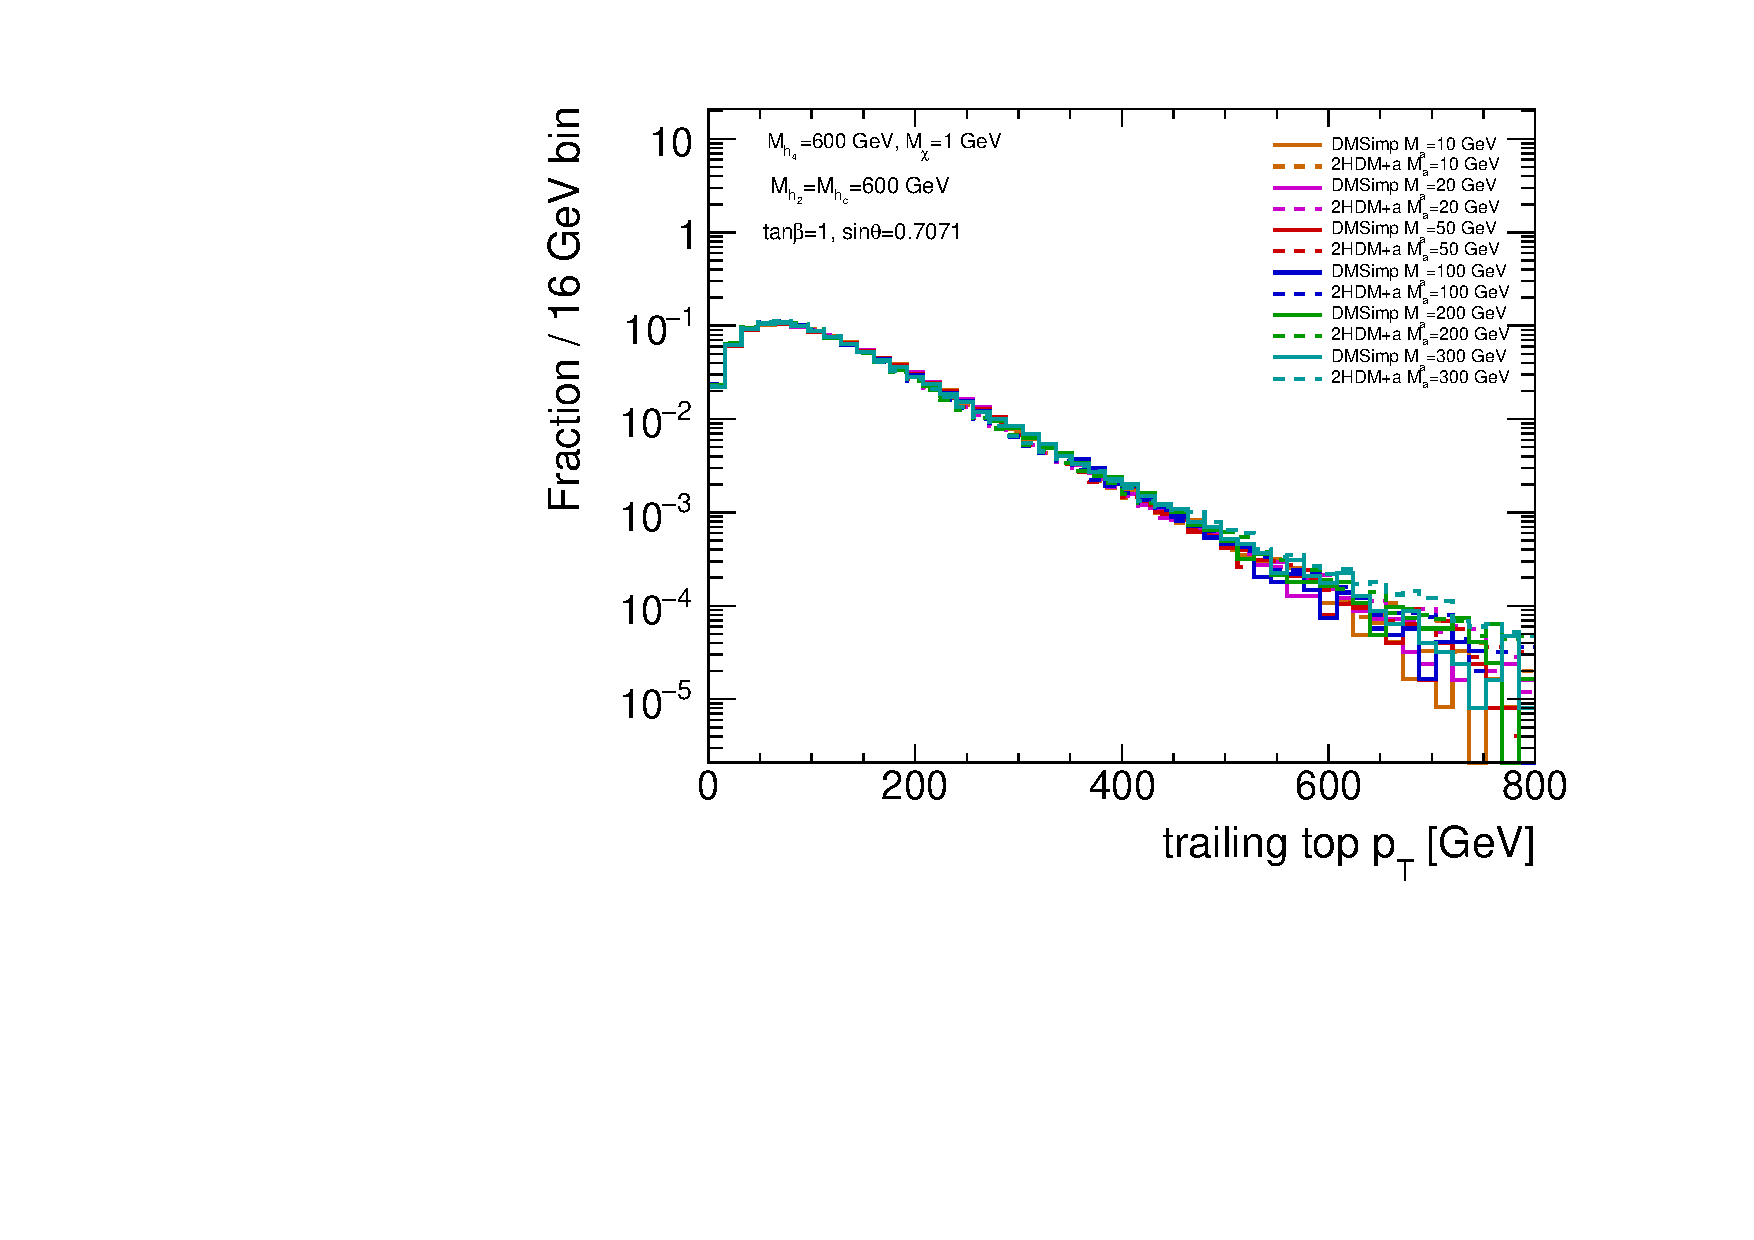
\includegraphics[width=\textwidth]{texinputs/04_grid/figures/DMHF/benchmarking/MDM_1_MA_600_sinp_0.7071_tanb_1.0_DMsimpV2HDMa/top2ptlog.pdf}
%    \caption{Trailing top $p_{T}$}
%  \end{subfigure}
%  \caption{The $E_{T}^{miss}$, leading and trailing top $p_{T}$ distributions for inclusive $t\bar{t}+\chi\bar{\chi}$ production generated from the \texttt{DMsimp} (solid) and the 2HDM+a (dashed) models with various values of $\mathrm{M_a}$. The 2HDM+a models are generated with the following model parameters:$\mathrm{M_A}=600$ GeV, $\mathrm{M_H}=\mathrm{M_{H^{\pm}}}=600$ GeV, $\tan\beta=1$, and $\sin\theta=0.7071$.}
%\label{fig:DMSimpV2HDMa}
%\end{figure}
%%%%%-----------------------------------------------------------------------------------------
%\subsubsection{Recasting existing tt+\met and bb+\met signatures}
%\label{subsub:hfttrecast}
%These two signatures are dominantly produced in diagrams involving the invisible decays of the two CP-odd scalars. 
%Their relevance is therefore determined by the two pseudoscalar masses, $m(A)$ and $m(a)$ and it is a function of 
%$sin\theta$ and $tan\beta$. 
%For both $bb$ and $tt$ associated productions, we find that the
%highest sensitivity of this signatures is obtained for high values of $sin\theta$.
%
%The 2HDM+a model is equivalent to a single pseudoscalar simplified
%model (DMF) when $A$ is much heavier than $a$, and therefore the
%former does not contribute to the considered final state. However,
%when the two mediators are closer in mass, the $pp\rightarrow ttA$
%contribution becomes more relevant  as it is possible to observe in 
%Figure~\ref{fig:mdd}, where the two models are compared
%assuming $m(A) = 750$ GeV and two different values
%for $m(a)$. An excellent agreement was observed between
%$DMSIMP$ and $2HDMp$ on parton-level variables sensitive 
%to the helicity structure of the interaction between top and the
%mediator\cite{Haisch:2016gry}, if the invariant mass of the two DM
%particles in the 2HDM is required to be smalle than 200(300)~GeV for
%$m(a)=150(300)$~GeV respectively, giving confidence that,
%once the contribution from $A$ production is separated, it is possible
%to fully map the $2HDM+a$ kinematics into the DMF simplified model. 
%
%
%\begin{figure}[htb]
%\begin{center}
%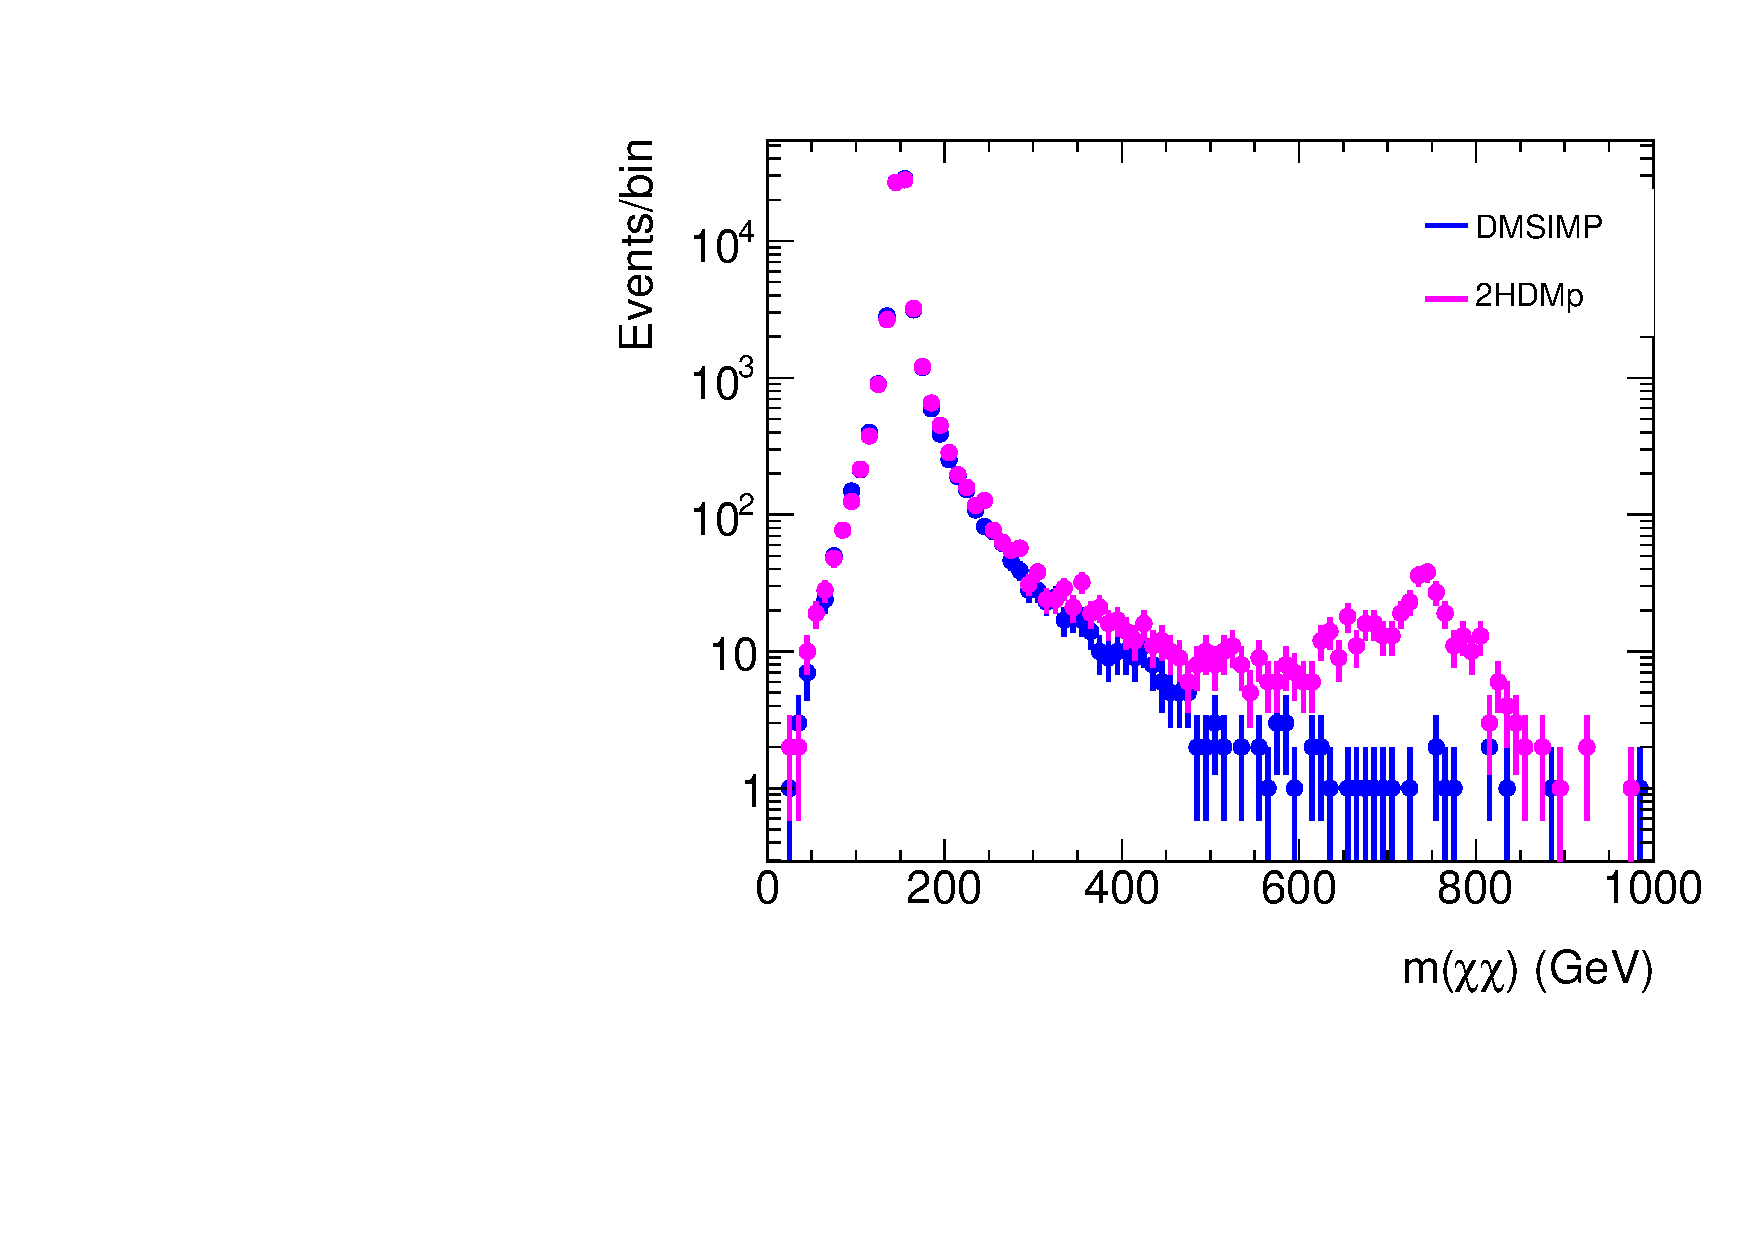
\includegraphics[width=0.48\textwidth]{texinputs/04_grid/figures/DMHF/mdd150.pdf}
%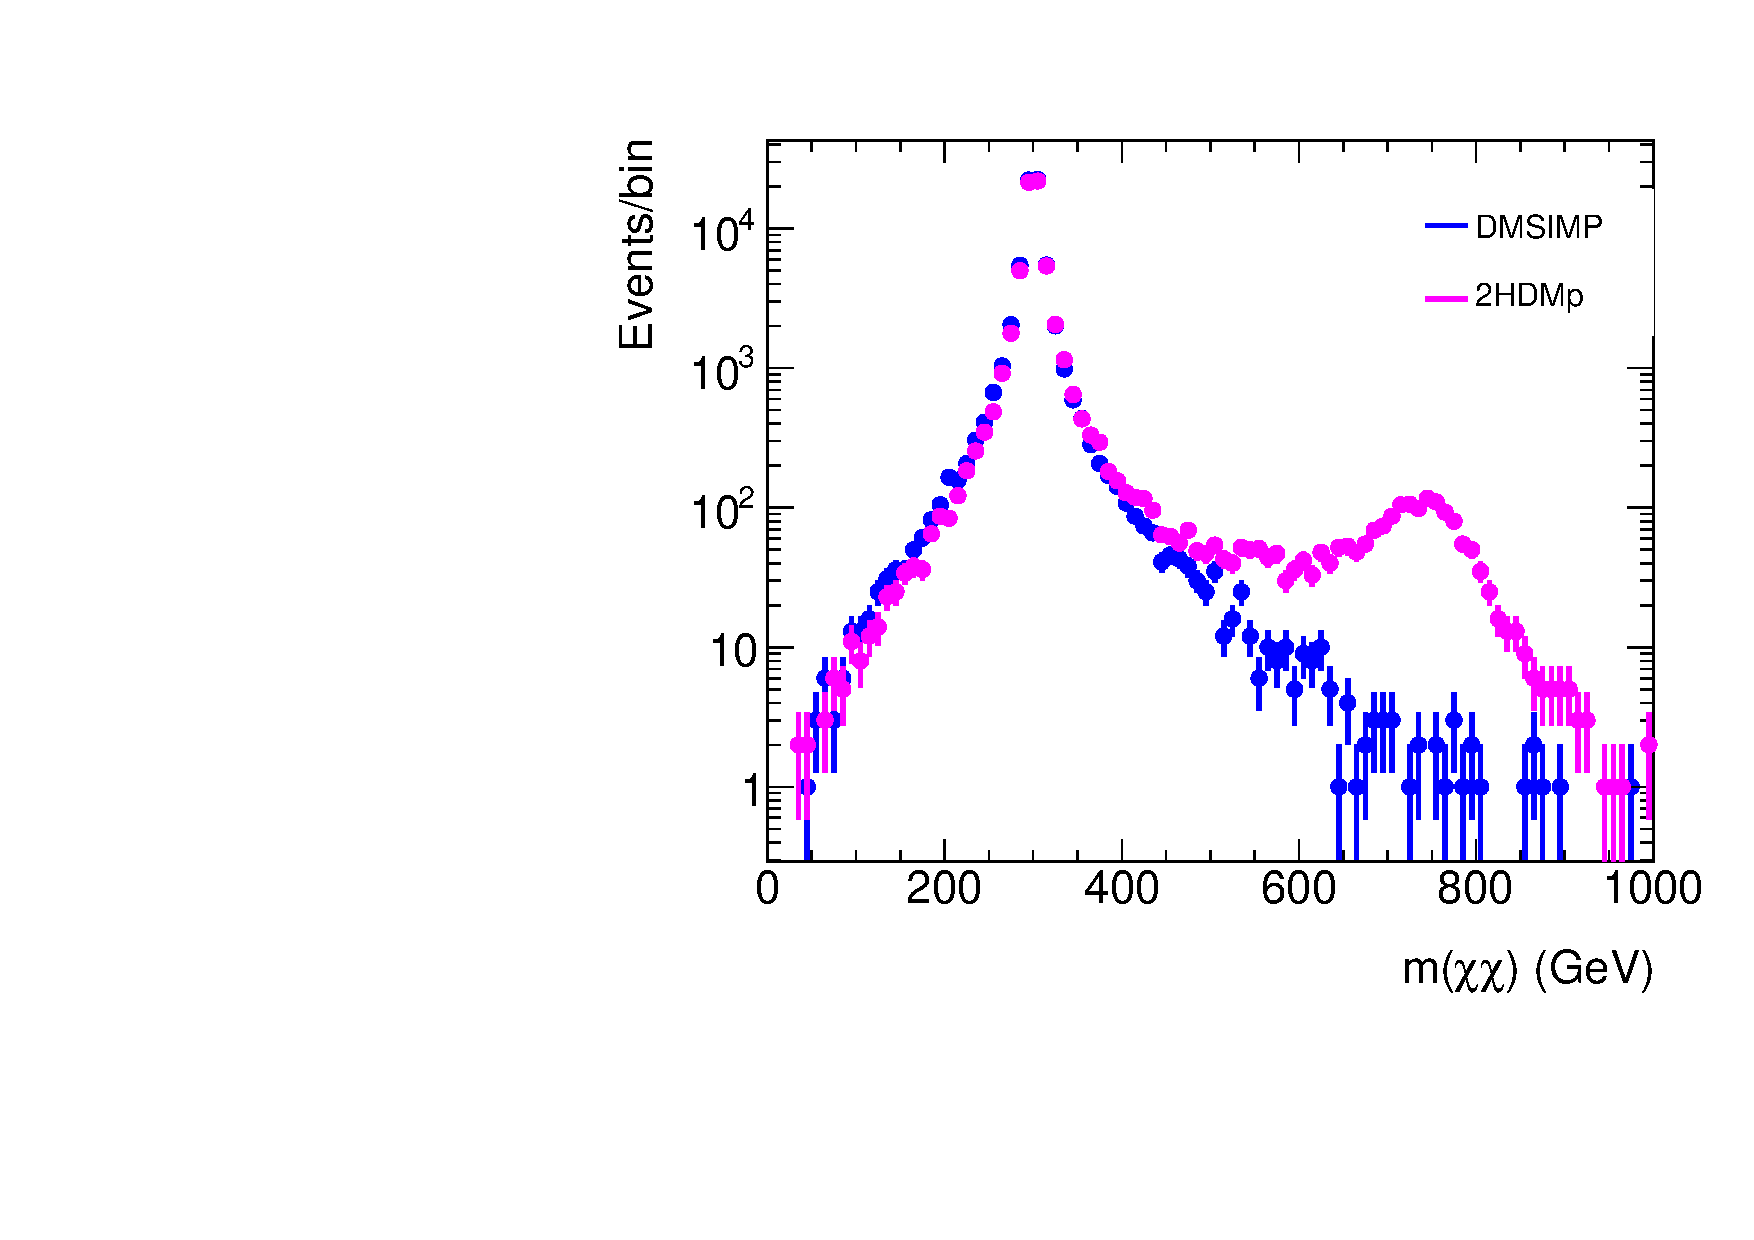
\includegraphics[width=0.48\textwidth]{texinputs/04_grid/figures/DMHF/mdd300.pdf}
%\caption{Comparison of $m(\chi\chi)$, the invariant mass of 
%the two DM particles for the $DMSIMP$ (blue) and the $2HDMp$ model (magenta). The plot on the left (right) shows the comparison for $m(a)=150(300)$~GeV
%respectively.}
%\label{fig:mdd}
%\end{center}
%\end{figure}
%
%This remapping is achieved by
%taking for each set of the parameters the 
%average of the selection acceptances for $m(A)$ and $M(A)$ as 
%calculated with $DMSIMP$ weighted by the respective 
%cross-section for $A$ ($\sigma_A$) and $a$ 
%($\sigma_a$) production, in formulas
%\begin{equation}
%Acc_{2HDM}(m(A),M(a))=\frac{\sigma_a \times Acc_{DMSIMP}(m(a))+
%\sigma_A \times Acc_{DMSIMP}(m(A))}{\sigma_a+\sigma_A}
%\label{rew}
%\end{equation}
%The acceptance in this case is a parton level implementation of the
%two-lepton analysis described in [arXiv:1710.11412].
%The acceptance estimated in this way is shown as red triangles 
%in Figure~\ref{fig:tbfin}, and an excellent agreement 
%can be seen with the acceptances evaluated directly on the 2HDM 
%samples. 
%\begin{figure}[htb]
%\begin{center}
%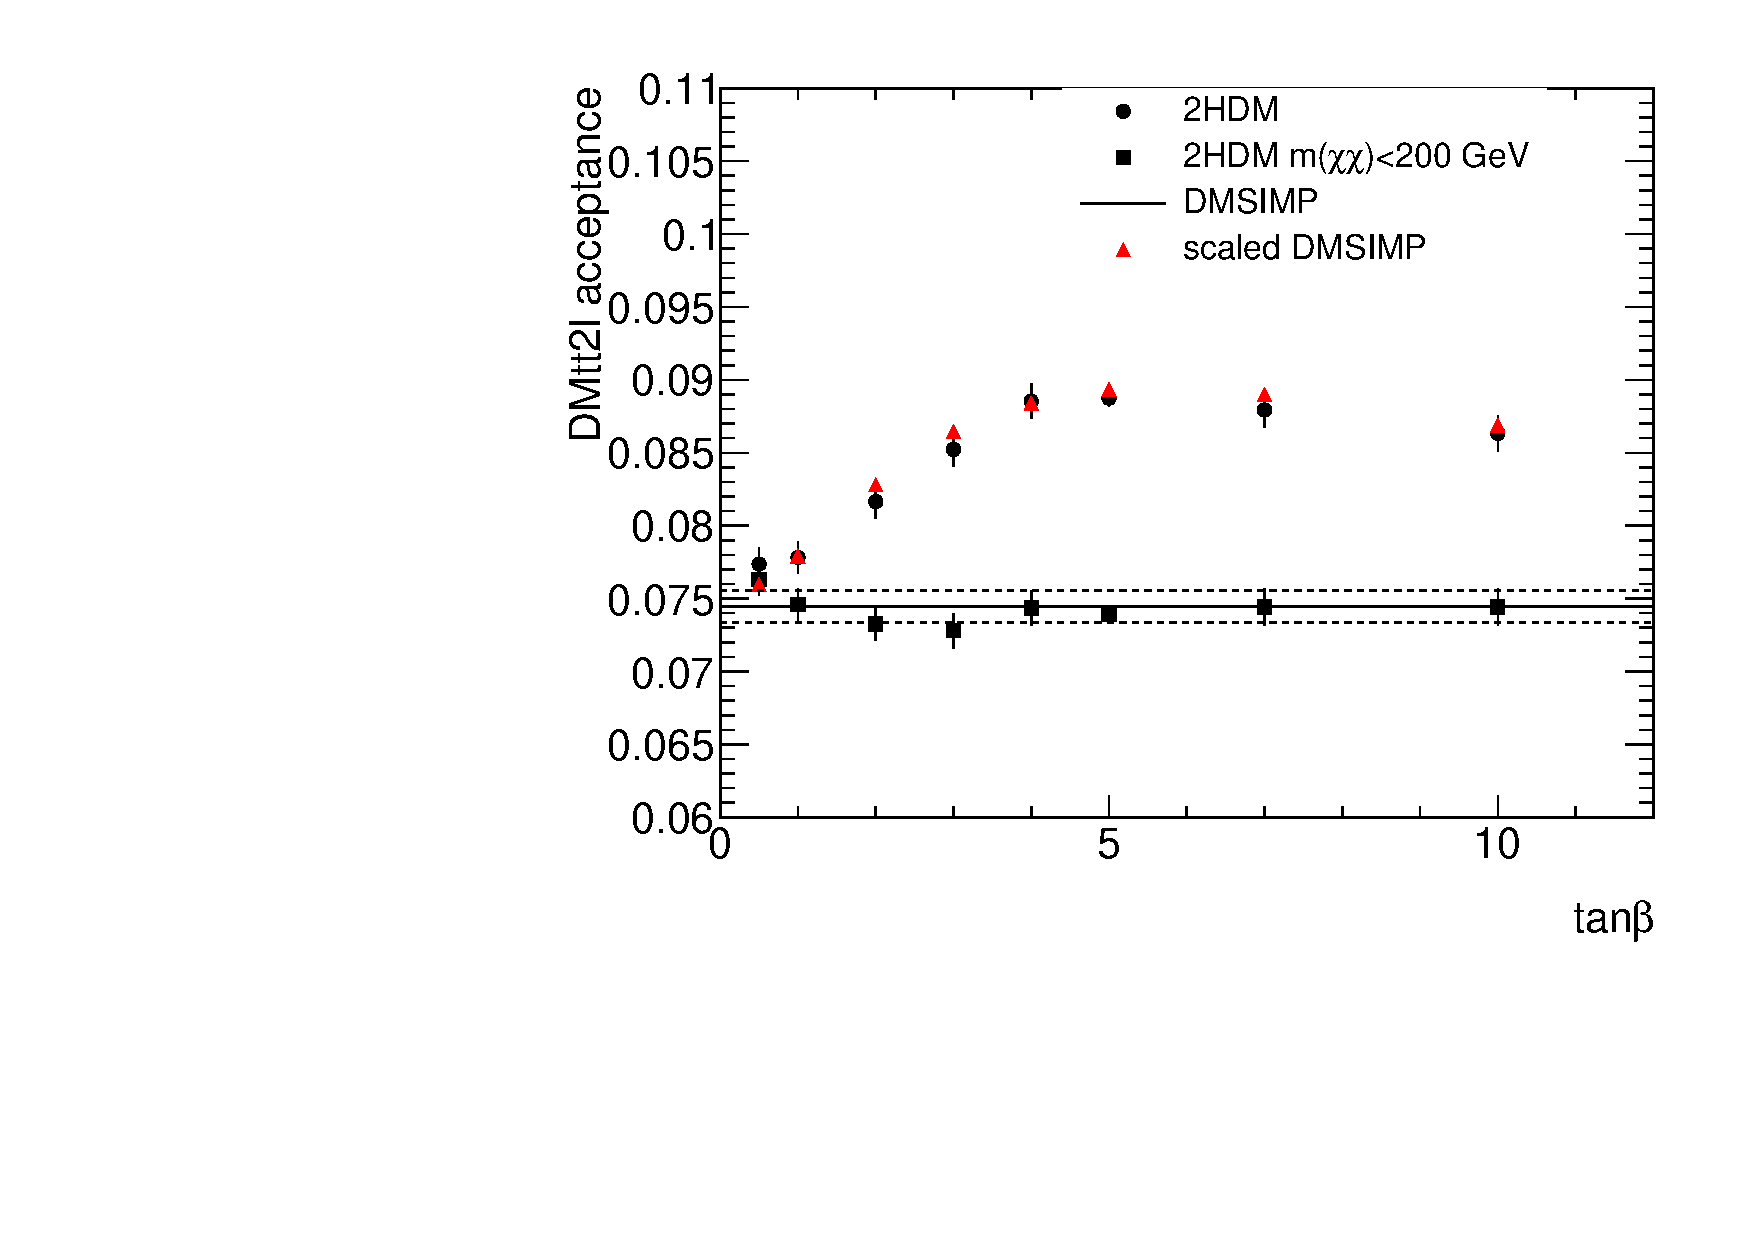
\includegraphics[width=0.7\textwidth]{texinputs/04_grid/figures/DMHF/plotacc_tb.pdf}
%\caption{Acceptance of the two-lepton analysis as a function of $\tan\beta$ 
%for the $2HDMp$ model (round markers), for the $2HDMp$ model 
%considering only events with $m(\chi\chi)<200$~GeV (square markers),
%and for the $DMSIMP$ model (full line) for a mediator
%mass of 150~GeV. The two dashed lines indicate
%the statistical error of the $DMSIMP$. The value of $m(A)$ is fixed at 
%600~GeV, and $\sin\theta=0.35$. 
%The acceptance 
%calculated from the $DMSIMP$ acceptance rescaled following the 
%prescription \ref{rew} (red triangles) is also shown.}
%\label{fig:tbfin}
%\end{center}
%\end{figure}
%The acceptance estimated in this way is shown as red triangles 
%in Figure~\ref{fig:tbfin}, and an excellent agreement 
%can be seen with the acceptances evaluated directly on the 2HDM 
%samples. Further validation were performed also on the acceptances calculated for zero and one lepton final states [1710.11412,1711.11520], 
%both as a function of $sin\theta$ and $tan\beta$ and can be observed in Fig~\ref{DMHF:pof}.
%Finally, the formula was succesfully tested also the situation in
%which $|m(A)-m(a)| \sim 50$ GeV, 
%implying the possibility of a large interference
%between the production of the two bosons.
%
%\begin{figure}
%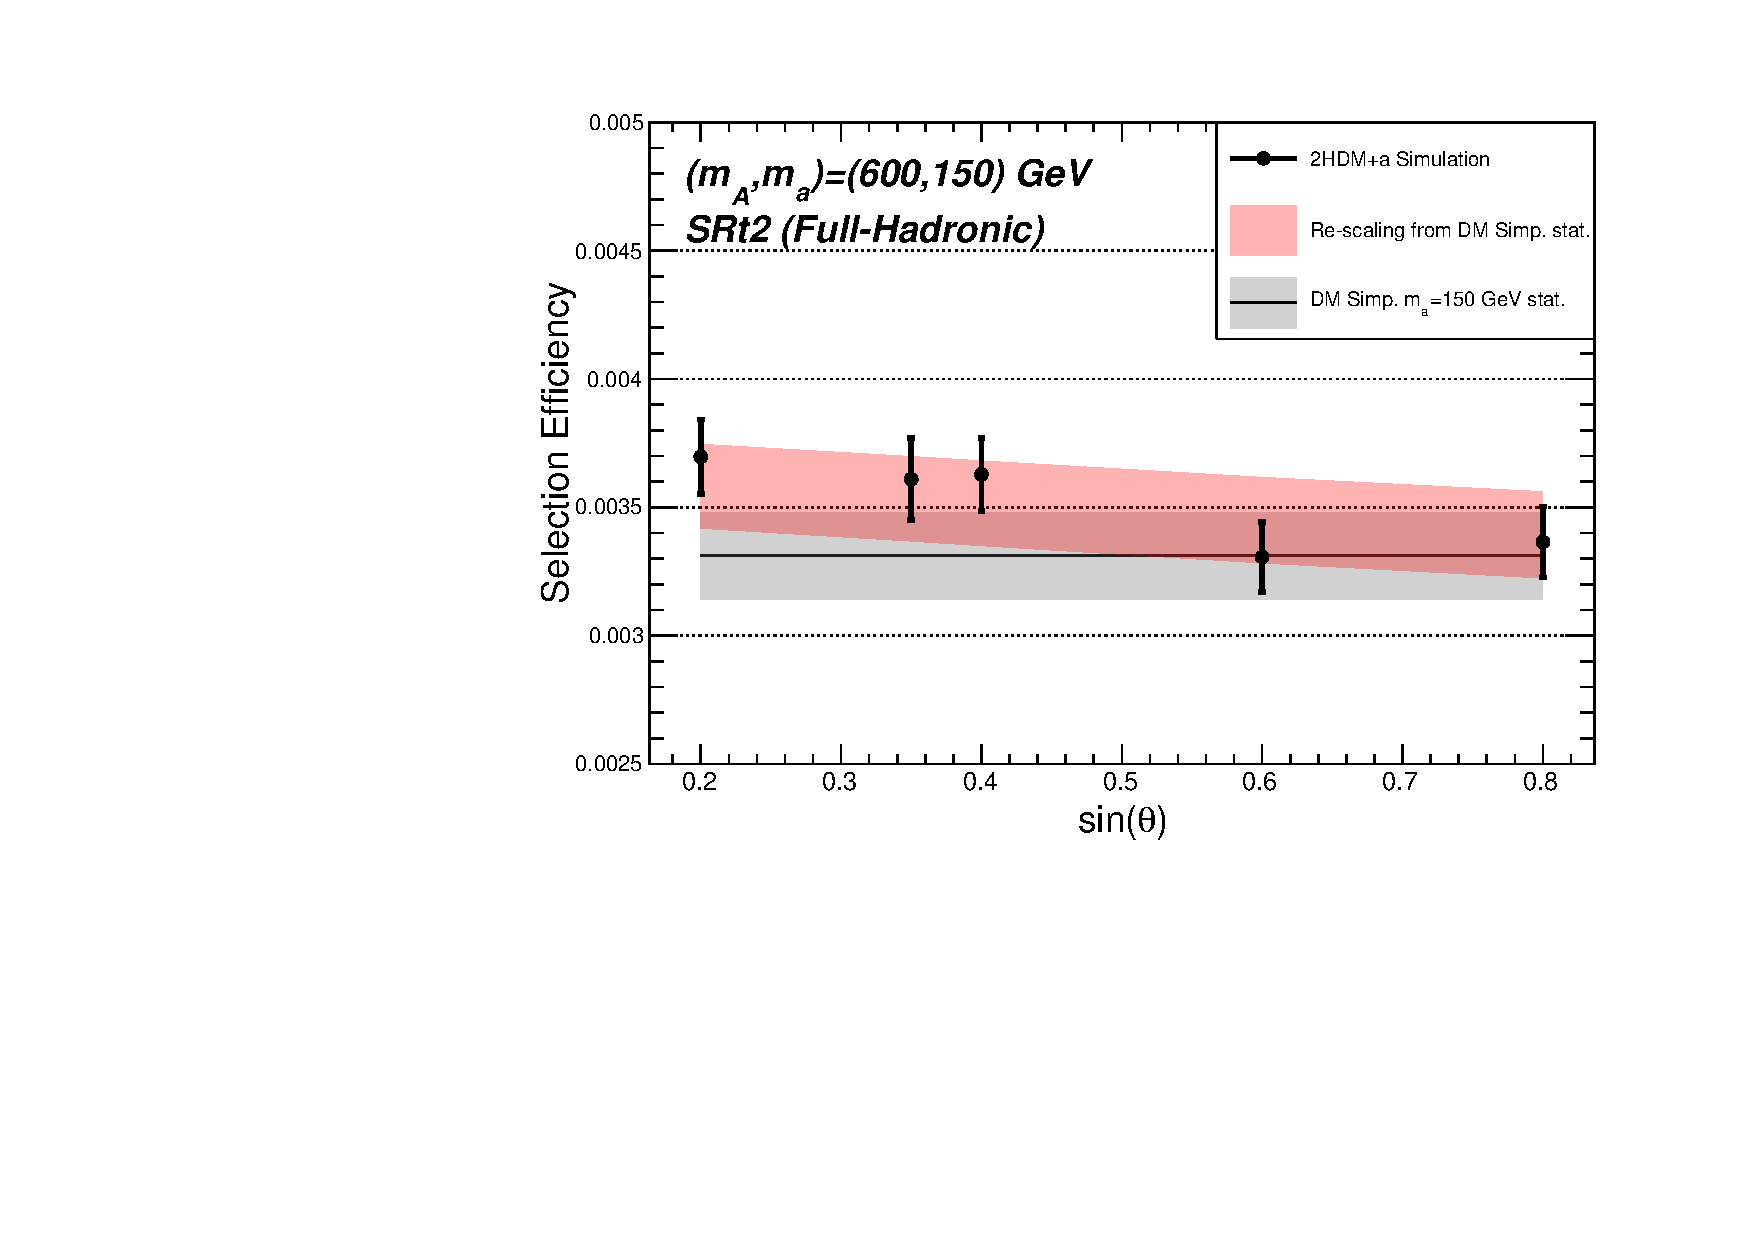
\includegraphics[width=.5\textwidth]{texinputs/04_grid/figures/DMHF/SRt2_600_150_sin}
%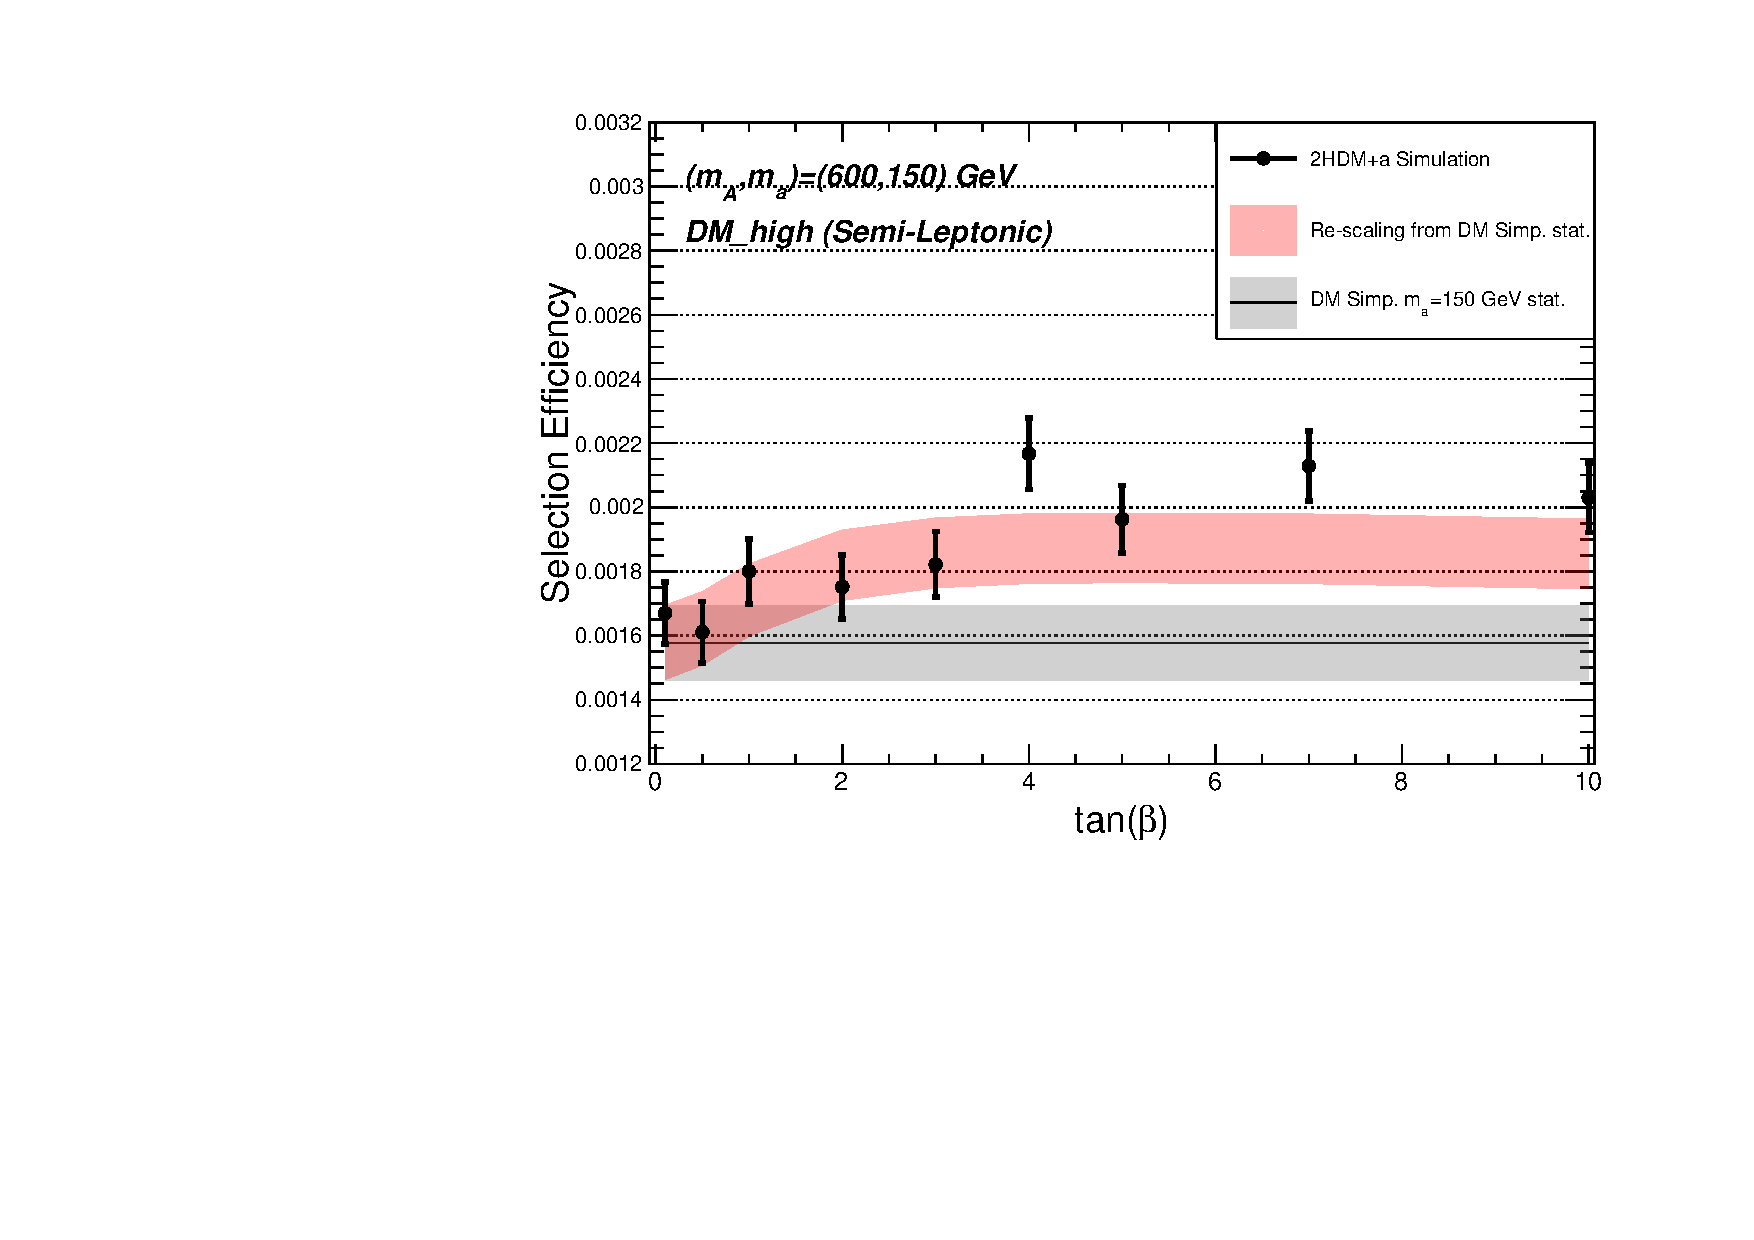
\includegraphics[width=.5\textwidth]{texinputs/04_grid/figures/DMHF/DM_high_600_150_tan}
%\caption{Validation of the re-scaling formula on zero and one lepton final states as a function of $tan\beta$ and $sin\theta$ parameters}
%\label{DMHF:pof}
%\end{figure}
%
%%%%-----------------------------------------------------------------------------------------
\subsubsection{Flavour scheme recommendations and studies}
\begin{figure} \centering
  \begin{subfigure}[b]{0.49\textwidth}           
    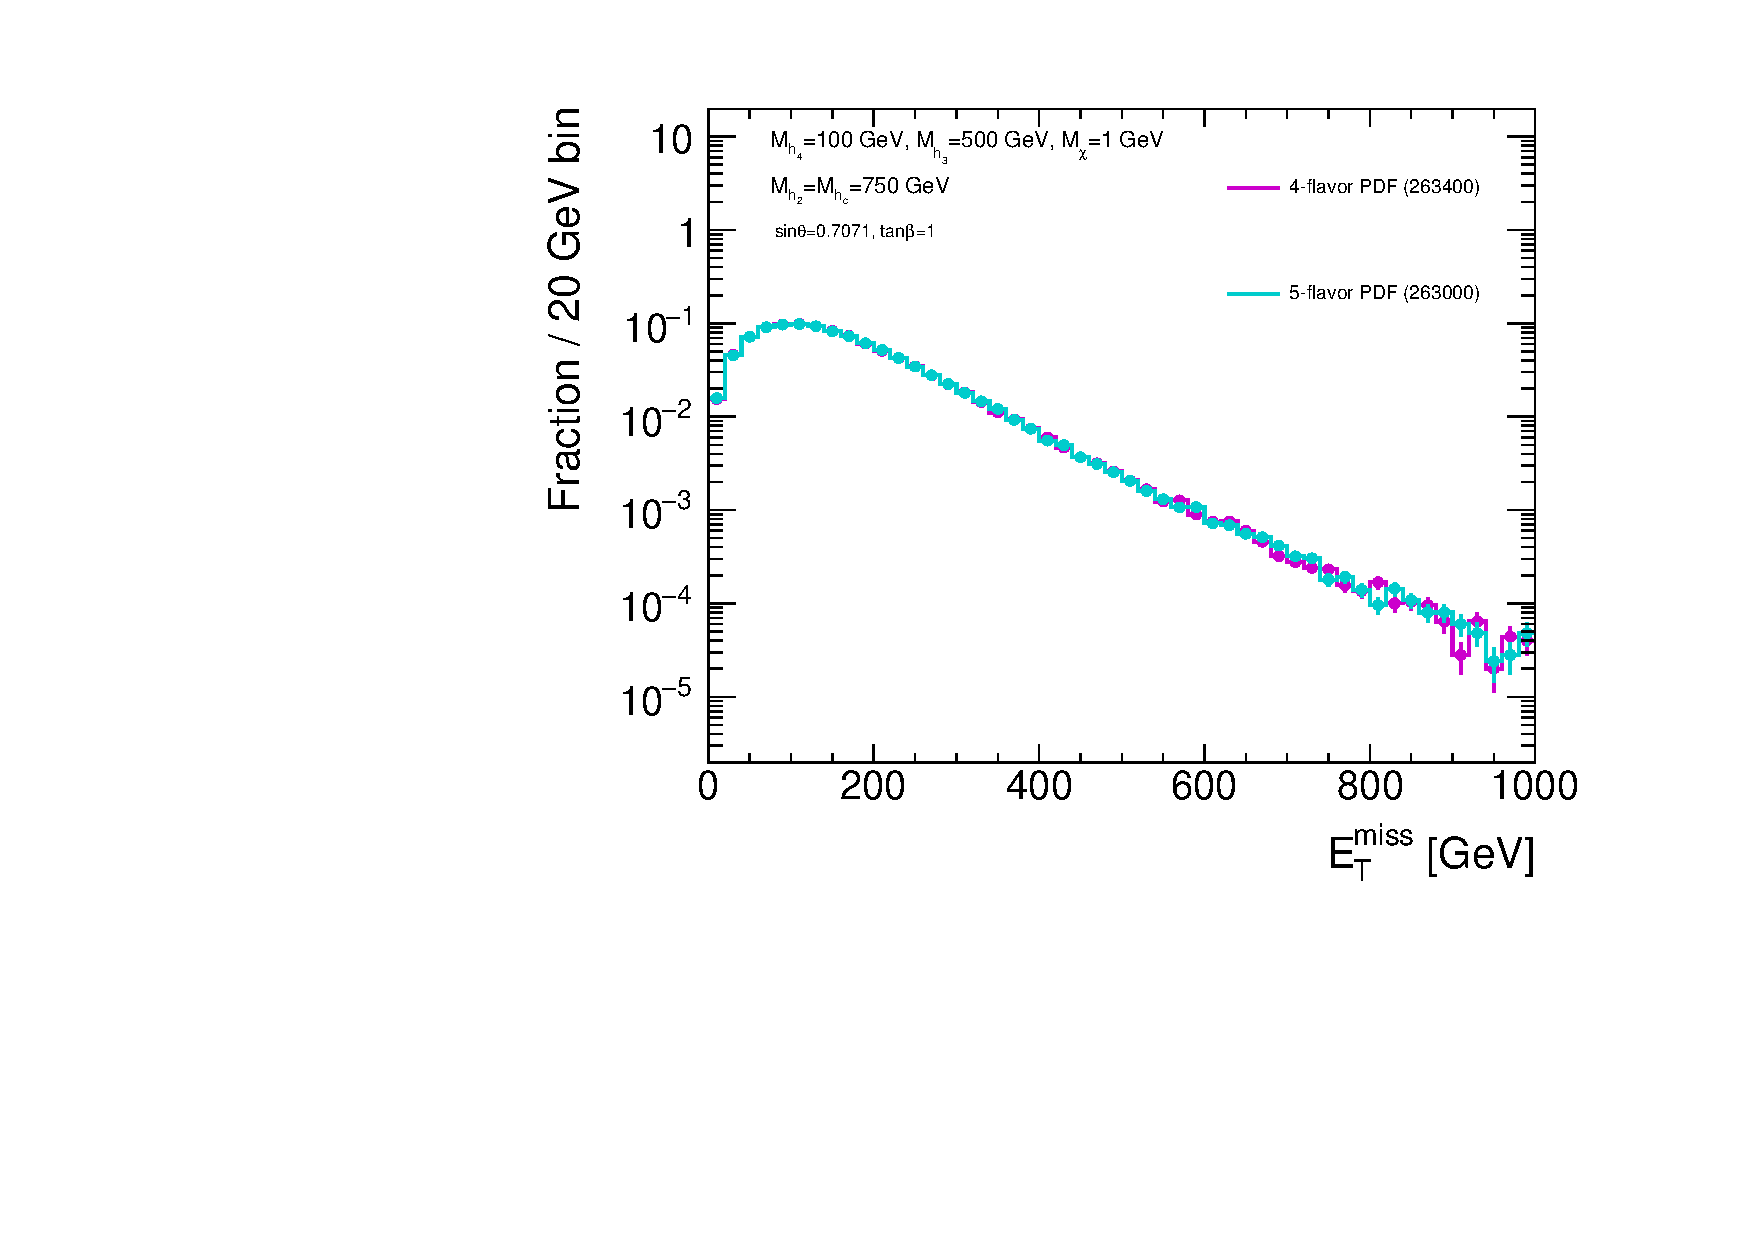
\includegraphics[width=\textwidth]{texinputs/04_grid/figures/DMHF/4v5flavour/MDM_1_Ma_100_MA_500_sinp_0.7071_tanb_1.0_4F_v_5F/metlog.pdf}
    \caption{$E_{T}^{miss}$}
  \end{subfigure}
  \begin{subfigure}[b]{0.49\textwidth}
    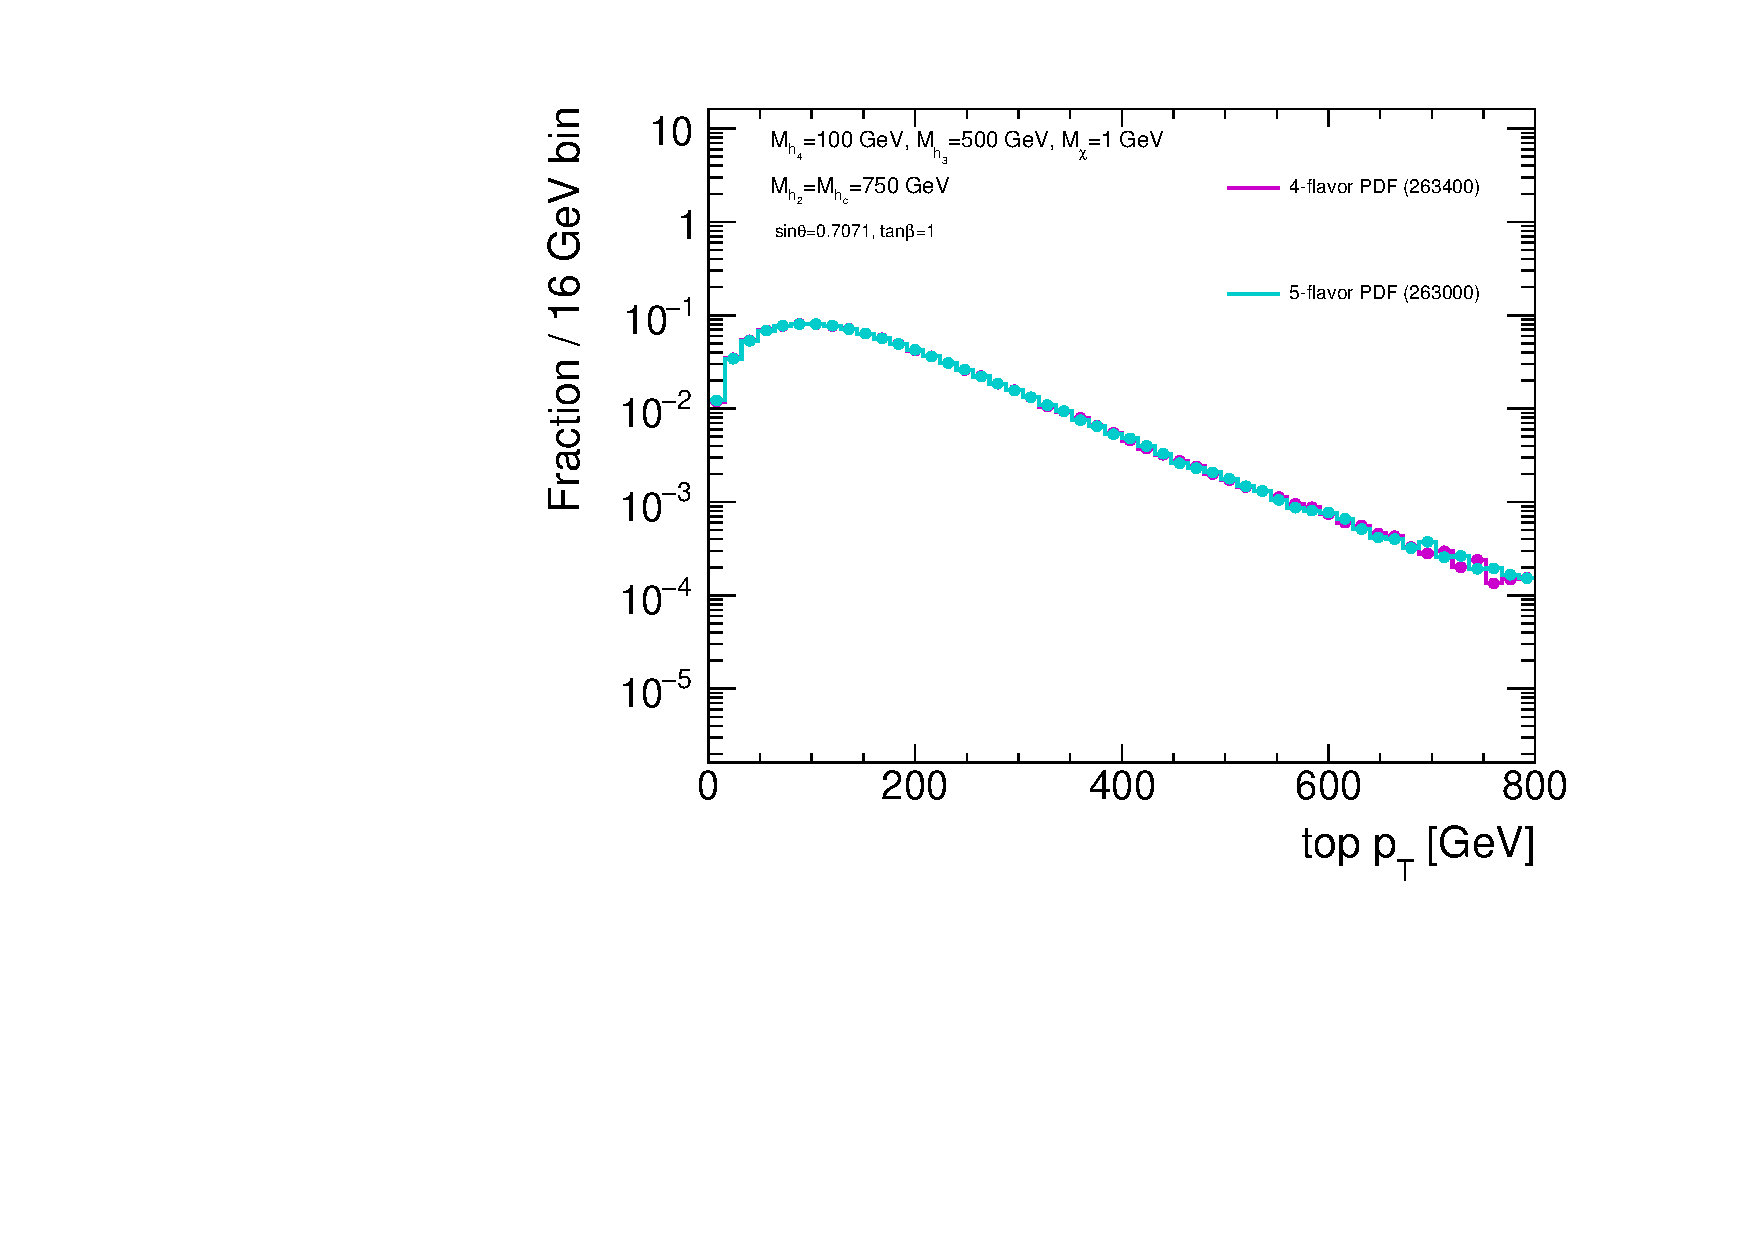
\includegraphics[width=\textwidth]{texinputs/04_grid/figures/DMHF/4v5flavour/MDM_1_Ma_100_MA_500_sinp_0.7071_tanb_1.0_4F_v_5F/topptlog.pdf}
    \caption{top $p_{T}$}
  \end{subfigure}
  \caption{$E_{T}^{miss}$ and top $p_{T}$ distributions for $M_{h_{4}}=100$ GeV, $M_{h_{3}}=500$ GeV, $M_{DM}=1$ GeV, $\mathrm{sin\theta}=0.7071$, and $\mathrm{tan\beta}=1$.}
  \label{fig:4v5_Ma100_MA500}
\end{figure}

\begin{figure} \centering
  \begin{subfigure}[b]{0.49\textwidth}           
    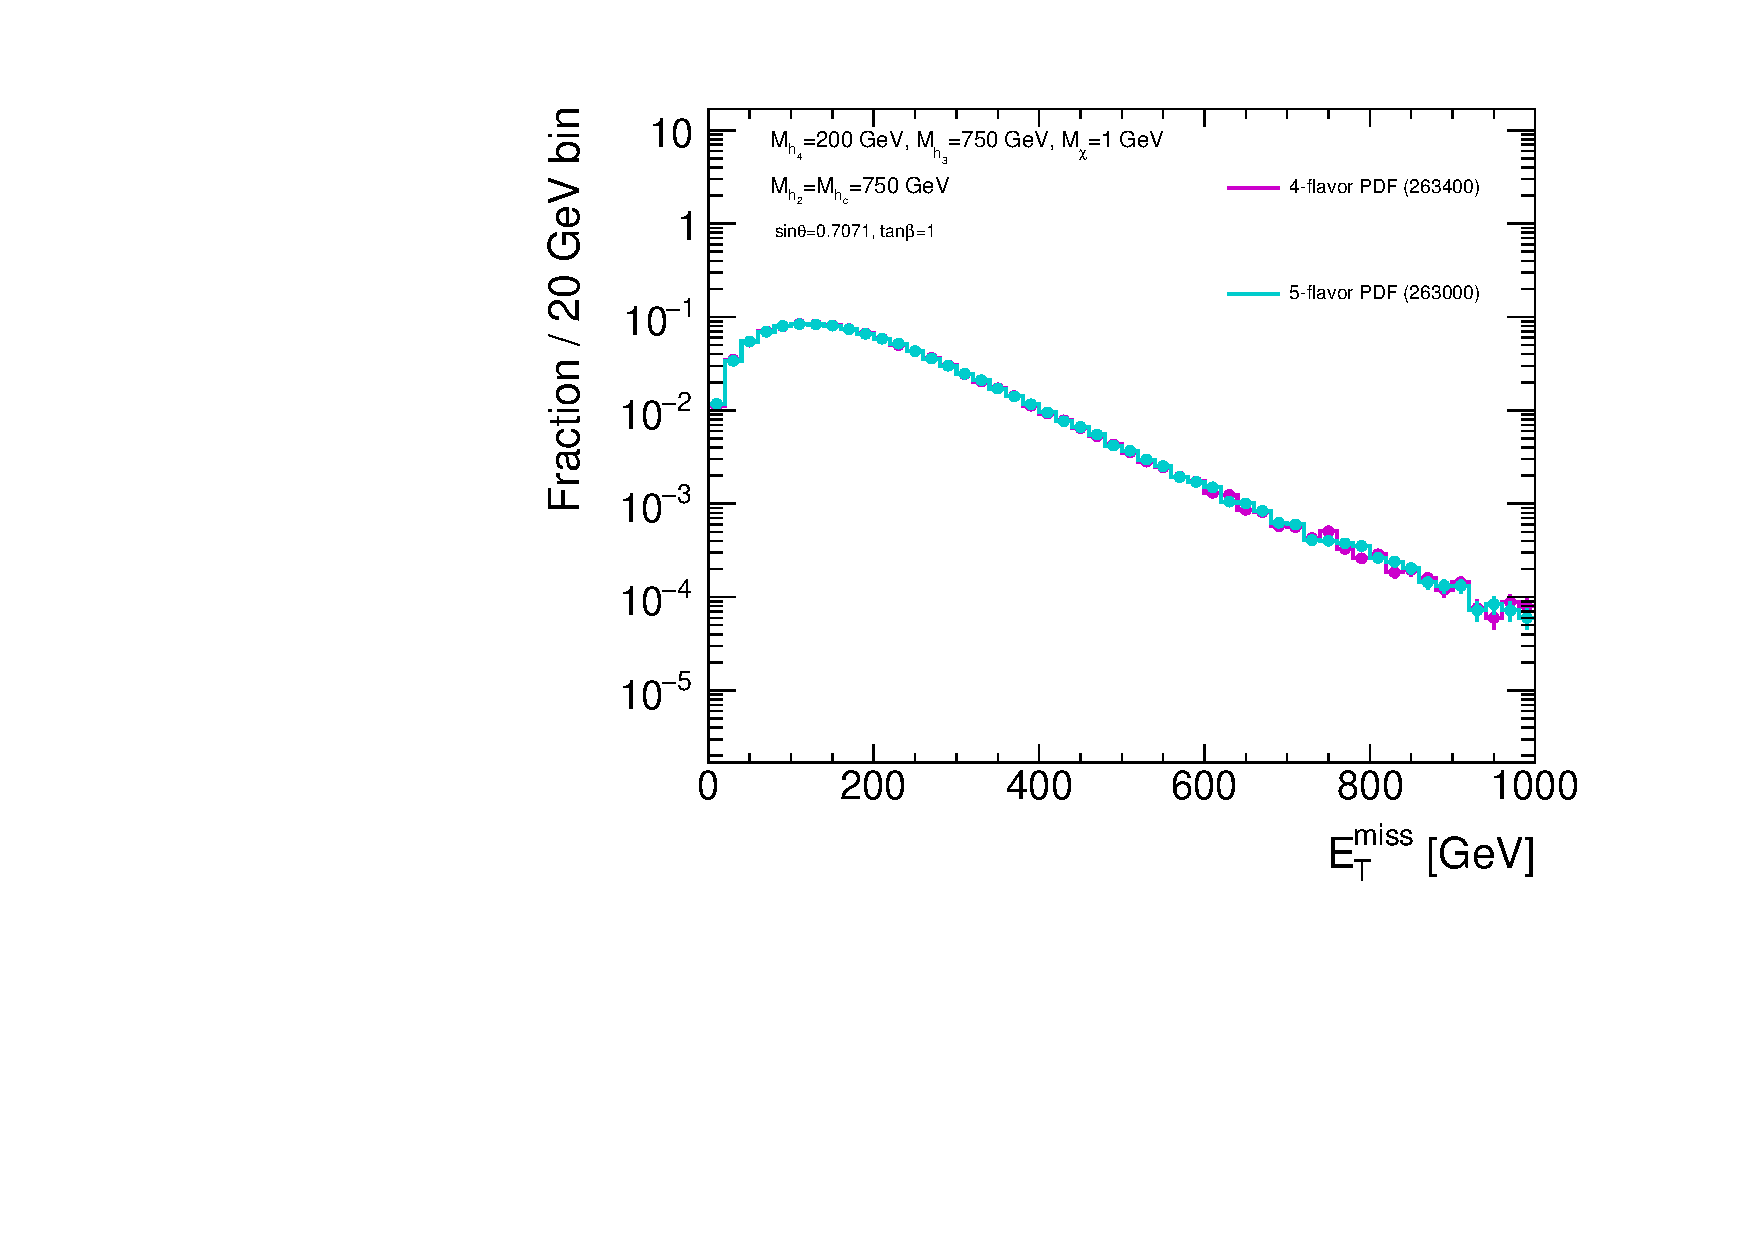
\includegraphics[width=\textwidth]{texinputs/04_grid/figures/DMHF/4v5flavour/MDM_1_Ma_200_MA_750_sinp_0.7071_tanb_1.0_4F_v_5F/metlog.pdf}
    \caption{$E_{T}^{miss}$}
  \end{subfigure}
  \begin{subfigure}[b]{0.49\textwidth}
    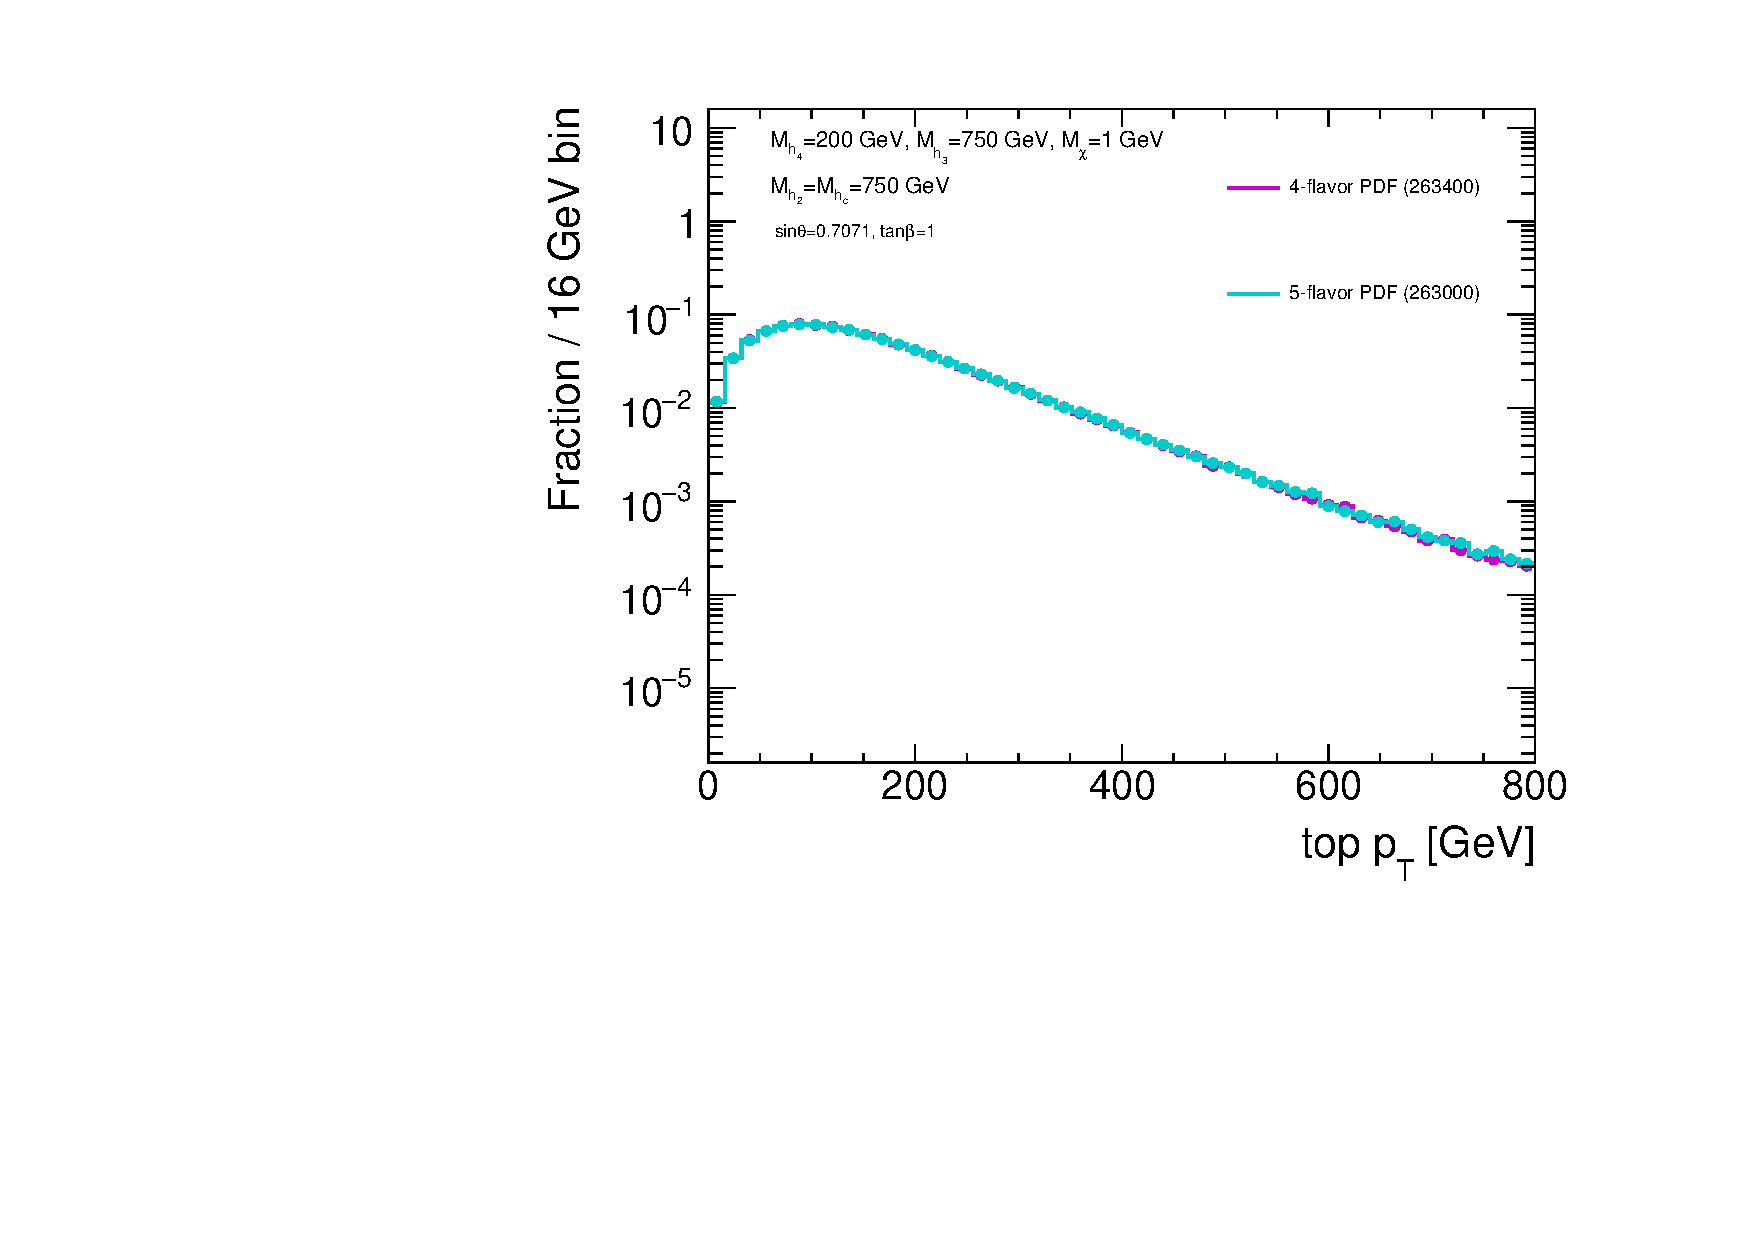
\includegraphics[width=\textwidth]{texinputs/04_grid/figures/DMHF/4v5flavour/MDM_1_Ma_200_MA_750_sinp_0.7071_tanb_1.0_4F_v_5F/topptlog.pdf}
    \caption{top $p_{T}$}
  \end{subfigure}
  \caption{$E_{T}^{miss}$ and top $p_{T}$ distributions for $M_{h_{4}}=200$ GeV, $M_{h_{3}}=750$ GeV, $M_{DM}=1$ GeV, $\mathrm{sin\theta}=0.7071$, and $\mathrm{tan\beta}=1$.}
  \label{fig:4v5_Ma200_MA750}
\end{figure}

\begin{figure} \centering
  \begin{subfigure}[b]{0.49\textwidth}           
    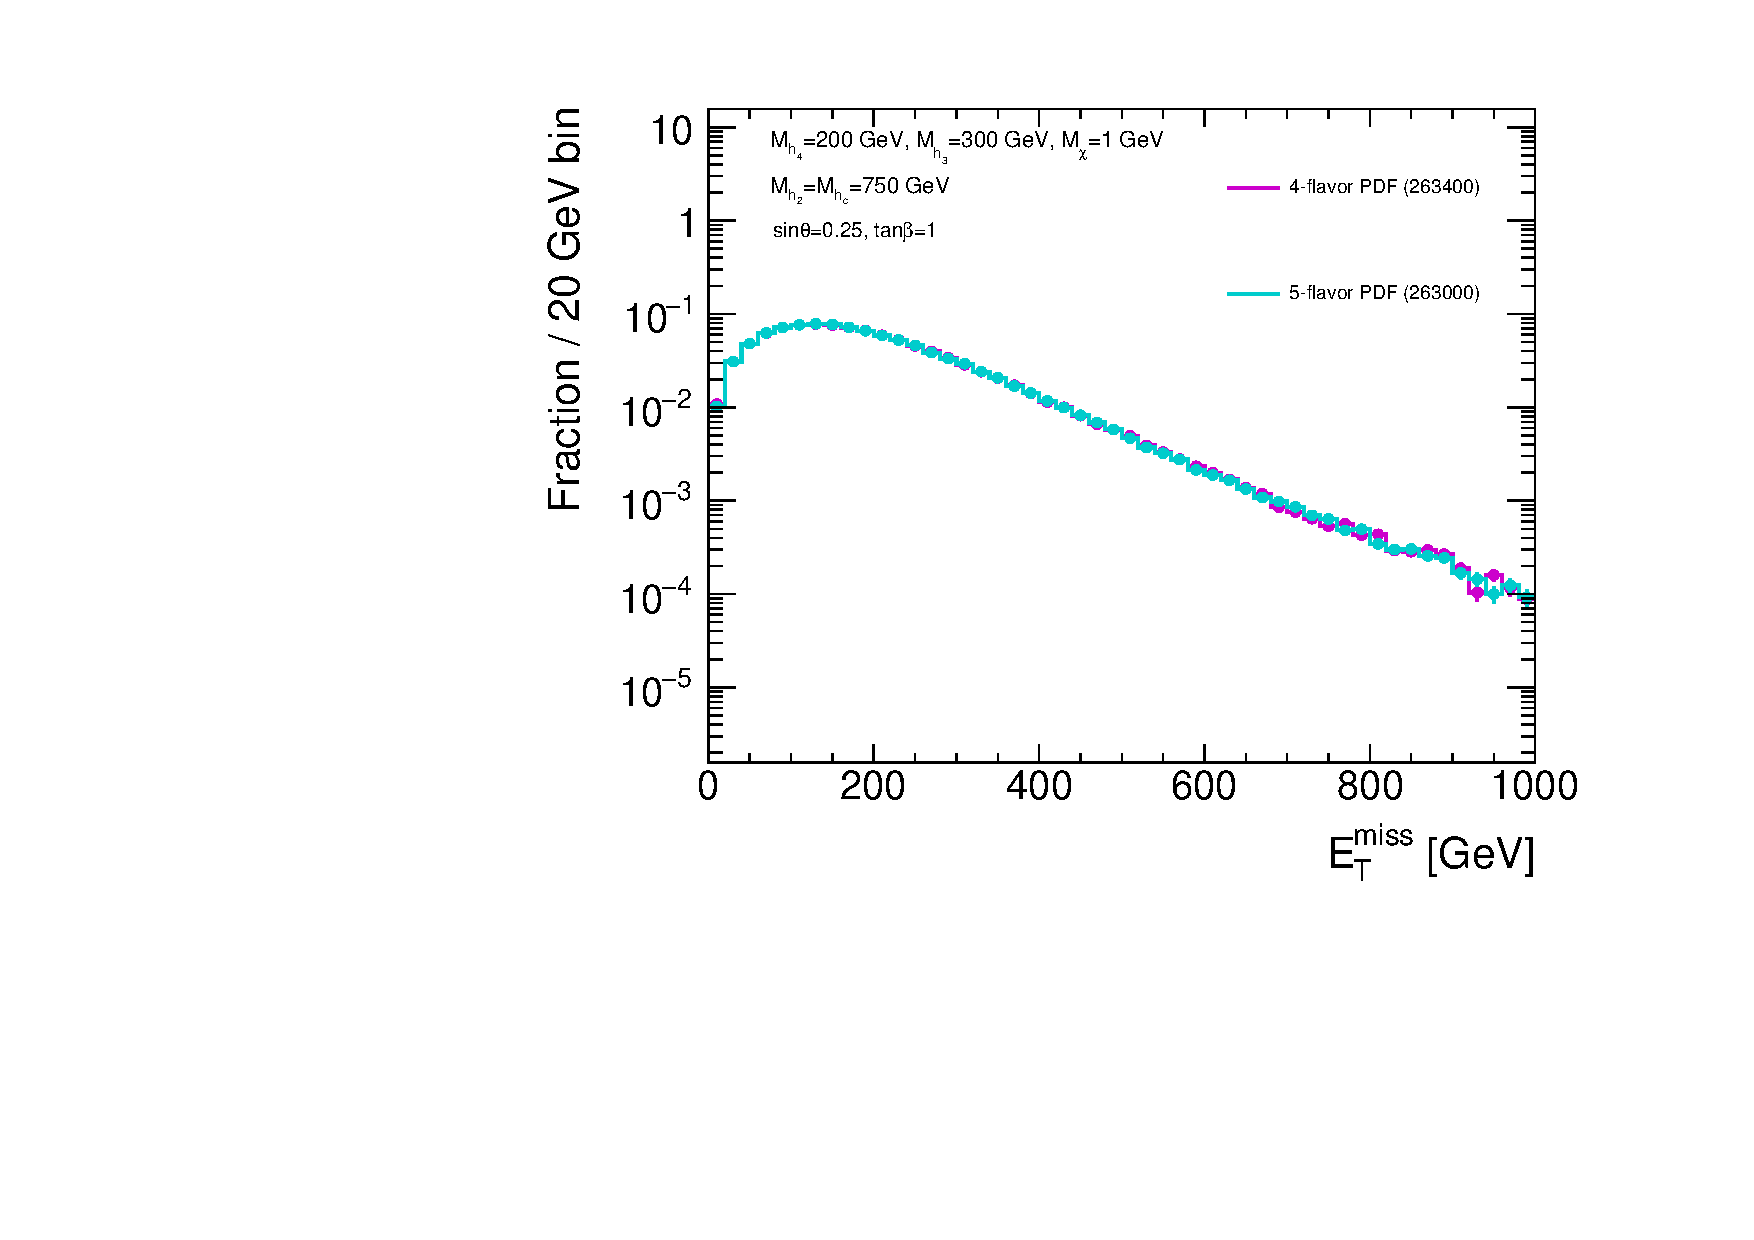
\includegraphics[width=\textwidth]{texinputs/04_grid/figures/DMHF/4v5flavour/MDM_1_Ma_200_MA_300_sinp_0.25_tanb_1.0_4F_v_5F/metlog.pdf}
    \caption{$E_{T}^{miss}$}
  \end{subfigure}
  \begin{subfigure}[b]{0.49\textwidth}
    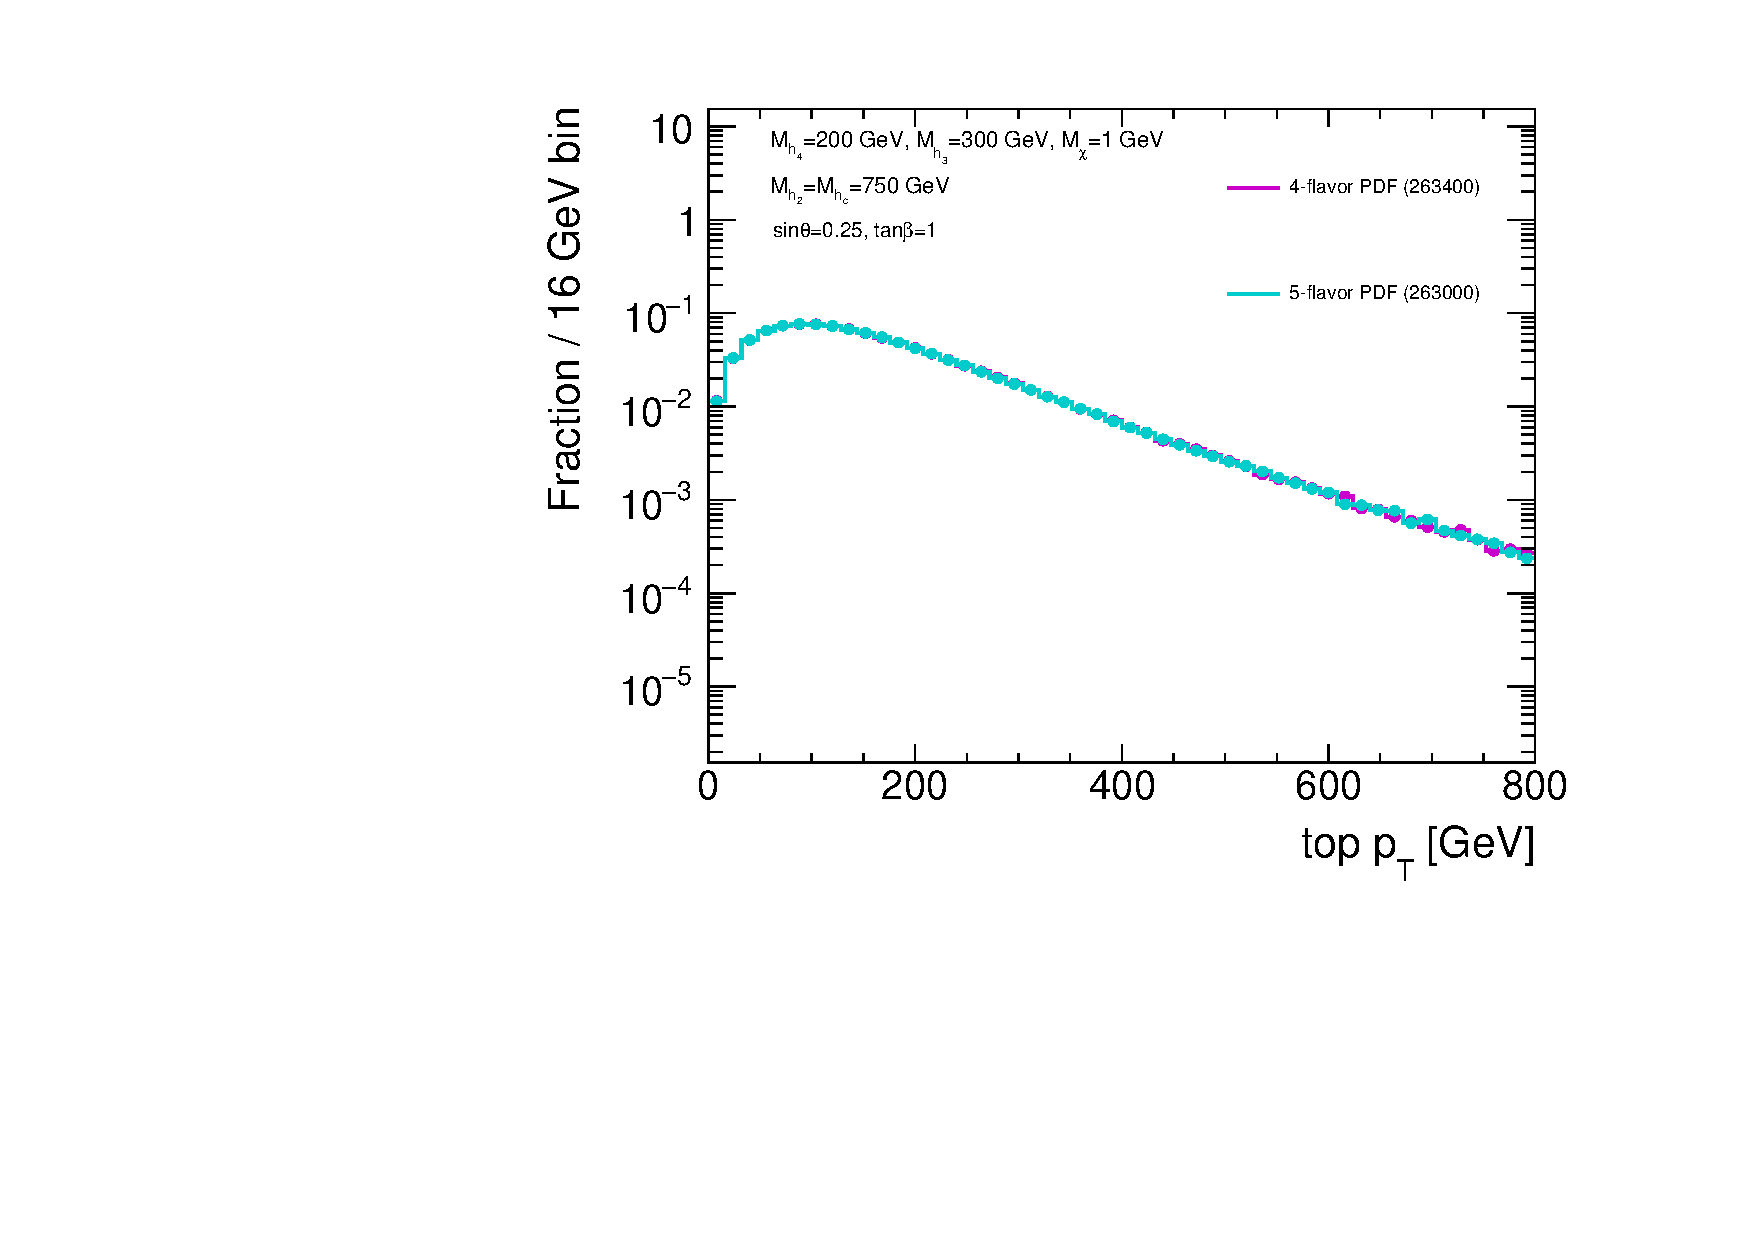
\includegraphics[width=\textwidth]{texinputs/04_grid/figures/DMHF/4v5flavour/MDM_1_Ma_200_MA_300_sinp_0.25_tanb_1.0_4F_v_5F/topptlog.pdf}
    \caption{top $p_{T}$}
  \end{subfigure}
  \caption{$E_{T}^{miss}$ and top $p_{T}$ distributions for $M_{h_{4}}=200$ GeV, $M_{h_{3}}=300$ GeV, $M_{DM}=1$ GeV, $\mathrm{sin\theta}=0.25$, and $\mathrm{tan\beta}=1$.}
  \label{fig:4v5_Ma200_MA300}
\end{figure}

The relevant kinematic distributions for $t\bar{t}+\chi\bar{\chi}$ associated production in the context of this model are shown to be independent from the choice of PDF flavour scheme. In Figures~\ref{fig:4v5_Ma100_MA500}$-$\ref{fig:4v5_Ma200_MA300}, the $E_{T}^{miss}$, which is taken to be the $p_{T}$ of the $\chi\bar{\chi}$ system, and the $p_{T}$ distribution of the top quarks is presented using the 4 and 5-flavour scheme. The 4-flavour LHAPDF ID is 263400 and corresponds to \texttt{NNPDF30\_lo\_as\_0130\_nf\_4}, and the 5-flavour LHAPDF ID is 263000 and corresponds to \texttt{NNPDF30\_lo\_as\_0130}. As demonstrated for various configurations of the 2HDM+a model parameters, the kinematics are not affected by the flavour scheme choice of PDF. Furthermore, the difference in cross-section between the 4-flavour and 5-flavour generated LO $t\bar{t}+\chi\bar{\chi}$ process is at the $2-3$\% level, as noted in Tab.~\ref{tab:4v5_xsec}.

Despite the lack of kinematic dependence on flavour scheme, it is recommended to use the 5-flavour PDF.\textcolor{red}{Add support/discussion and references}

\begin{table}[htbp]
  \begin{tabular}{|c|c|c|c|c|c|c|}
    \hline
    $\mathrm{M_{h_{2}}},\mathrm{M_{h_{c}}}$ [GeV] & $\mathrm{M_{h_{3}}}$ [GeV] & $\mathrm{M_{h_{4}}}$ [GeV] & $\sin\theta$ & $\tan\beta$ & 4F $\sigma$ (pb) & 5F $\sigma$ (pb) \\
    \hline \hline
    750 & 500 & 100 & 0.7071 & 1 & 0.0988596 & 0.0964933 \\
    \hline
    750 & 750 & 200 & 0.7071 & 1 & 0.0445115 & 0.043149 \\
    \hline
    750 & 300 & 200 & 0.25 & 1 & 0.0310152 & 0.0300196 \\ 
    \hline
  \end{tabular}
  \caption{Configurations of the 2HDM+a model used to generate the $t\bar{t}+\chi\bar{\chi}$ process at LO and the corresponding cross-sections from the 4-flavour (4F) and 5-flavour (5F) PDF.}
  \label{tab:4v5_xsec}
\end{table}
%%%%-----------------------------------------------------------------------------------------
\paragraph{Motivations for an high $tan\beta$ scan for bb+\met}

The projection of sensitivity in $tan\beta$ for benchmark \#2,  based on the CMS results for bb+MET [arXiv:1706.02581]
are shown in Figure~\ref{DMHF:bbscan}. The reach for an upper bound on tan(beta) with bb+MET shows 
good potential, for $tan\beta$ values above 10. 

\textbf{Say something about high width for H?}

\begin{figure}
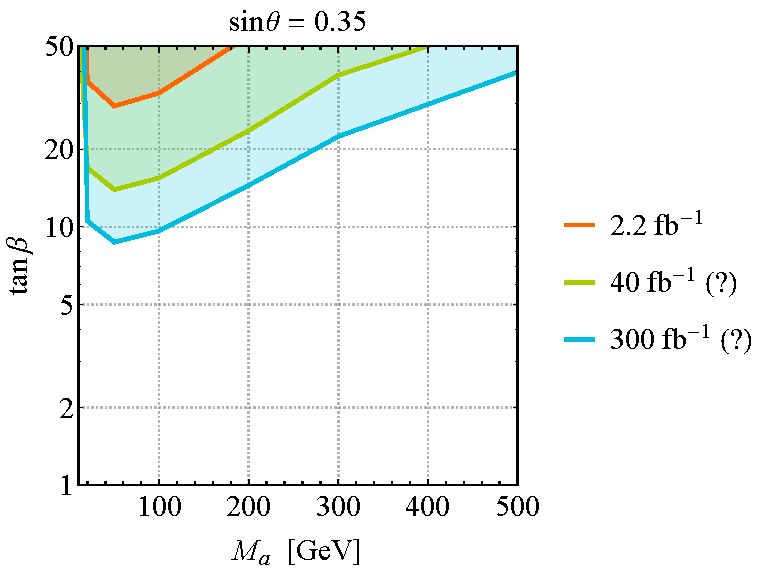
\includegraphics[width=.6\textwidth]{texinputs/04_grid/figures/DMHF//MAvsTB.pdf}
\caption{Sensitivity projection for benchmark \#2 based on the CMS results for bb+MET [arXiv:1706.02581].}
\label{DMHF:bbscan}
\end{figure}



%%%%-----------------------------------------------------------------------------------------
%%%%-----------------------------------------------------------------------------------------
%%%%-----------------------------------------------------------------------------------------
\clearpage
\subsubsection{Motivation for a dedicated tW+\met search}

The sensitivity of the LHC experiments to the associated 
production of dark matter with a single top has been recently studied \cite{Pani:2017qyd} in the framework
of an extension of the standard model featuring two Higgs doublets and
an additional pseudoscalar mediator. 
This study extends the work of previous literature \cite{Pinna:2017tay}, which demostrated using
a simplified model that the consideration of final states involving a single top quark and DM (DM$t$)
increases the coverage of existing analyses targeting the DM$t\bar t$ process.  

\begin{figure}
\begin{center}
\begin{subfigure}{.23\textwidth}\centering
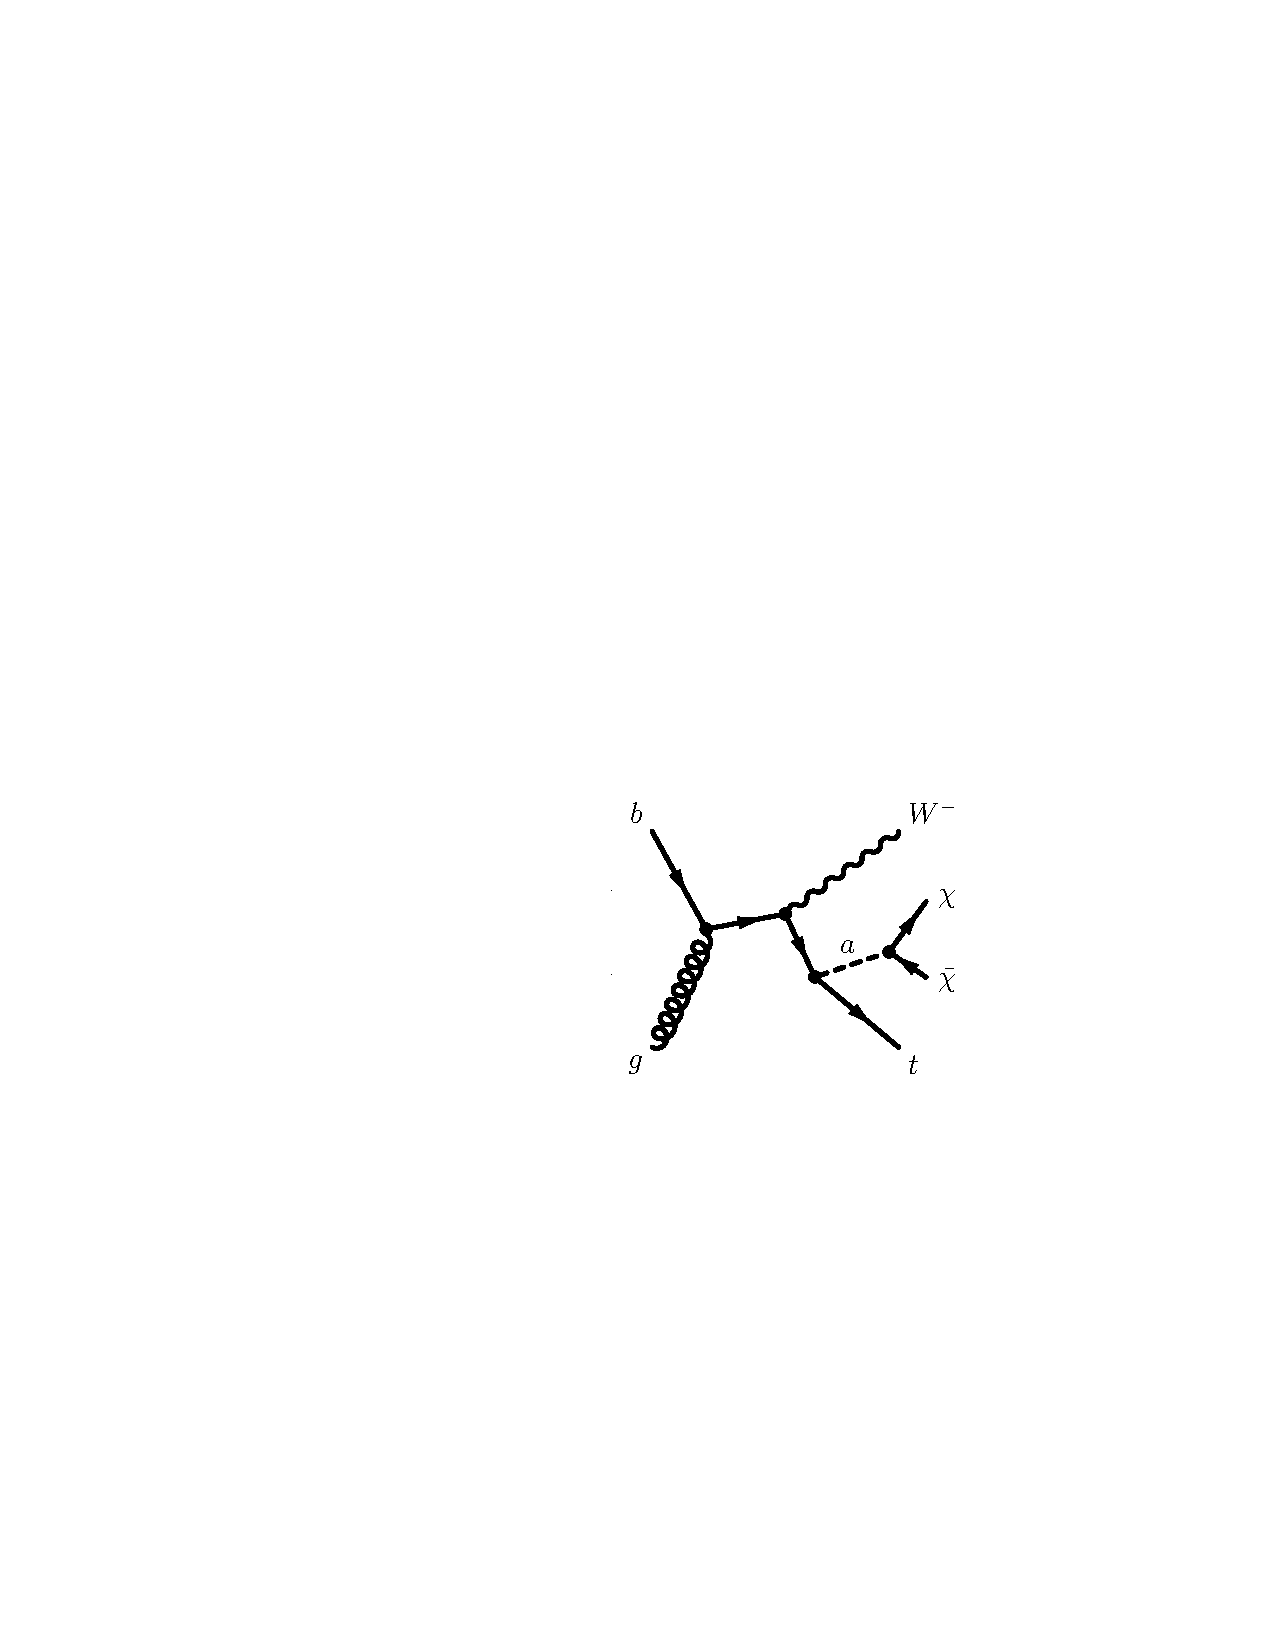
\includegraphics[width=\textwidth]{texinputs/04_grid/figures/DMHF/Pfeyn_tw2}
\caption{}
\end{subfigure}
\begin{subfigure}{.23\textwidth}\centering
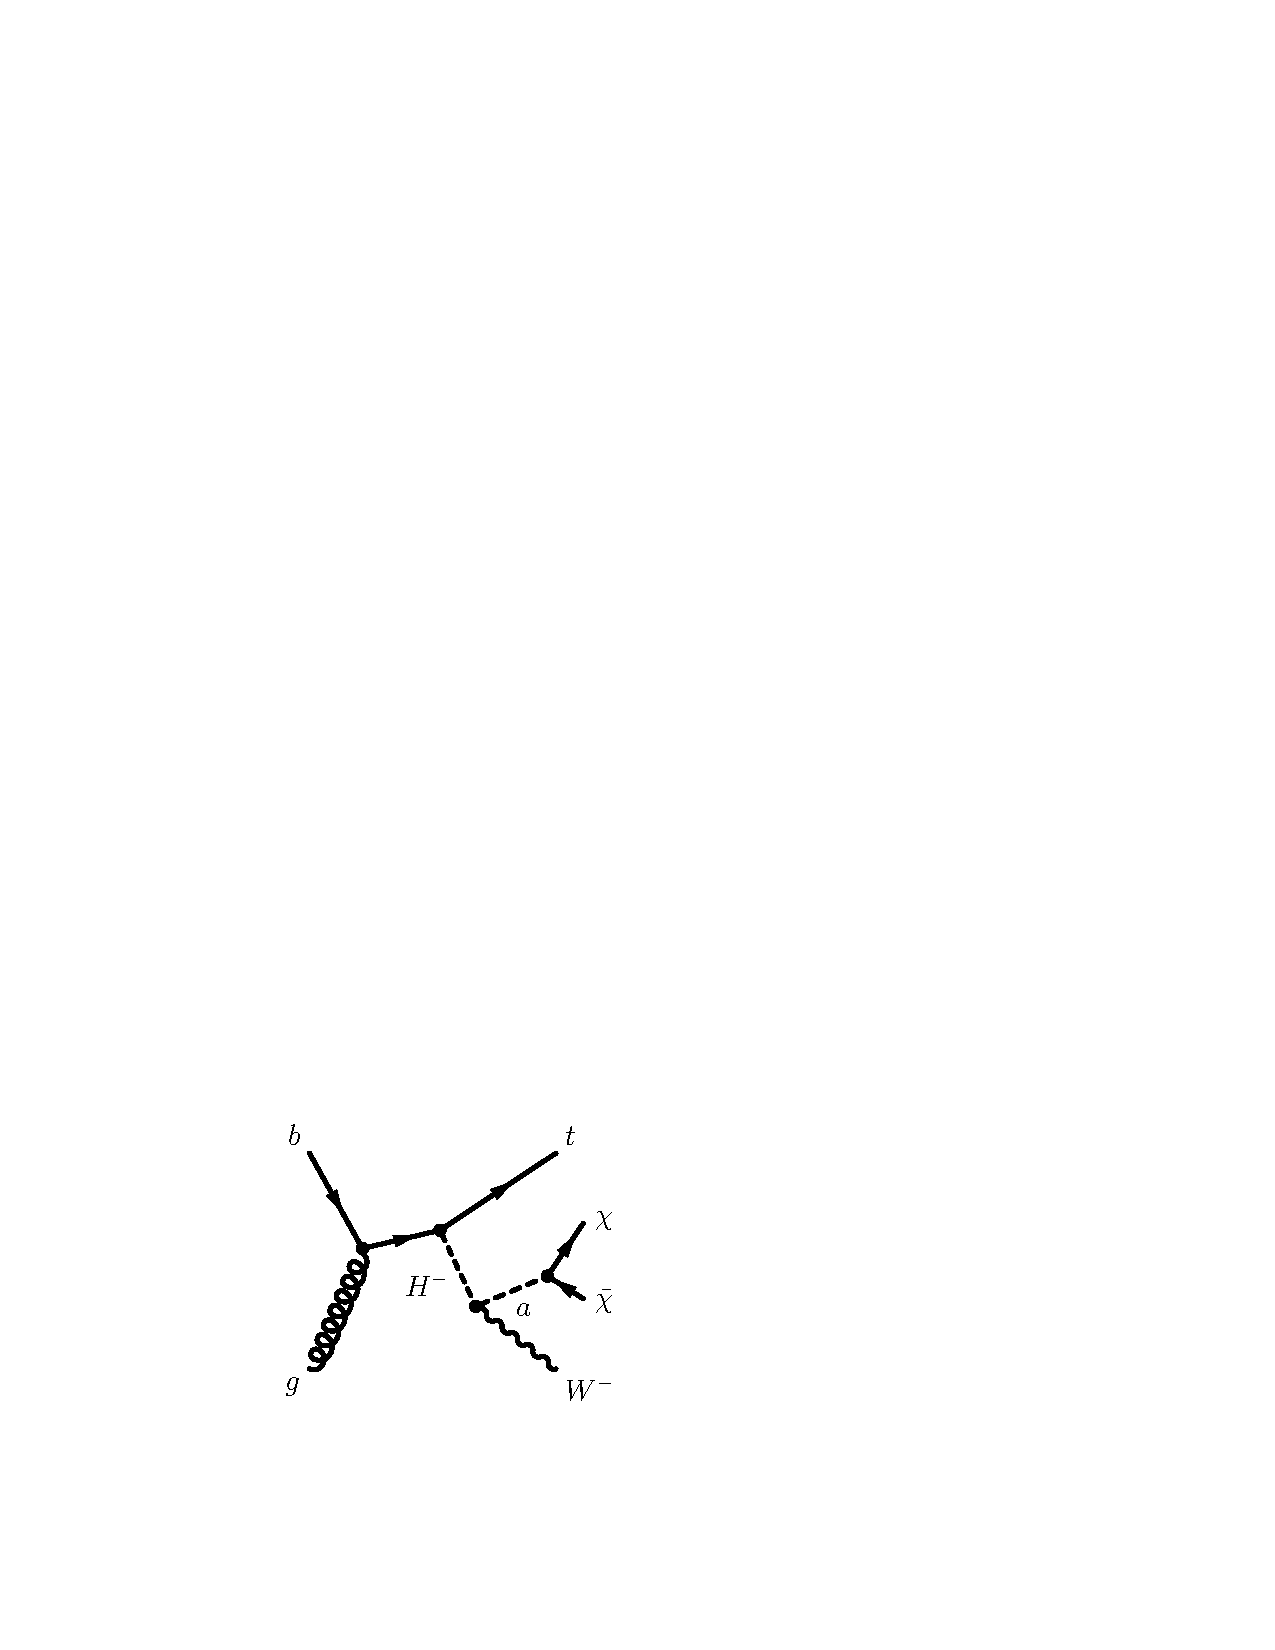
\includegraphics[width=\textwidth]{texinputs/04_grid/figures/DMHF/Pfeyn_tw1}
\caption{}
\end{subfigure}
\begin{subfigure}{.23\textwidth}\centering
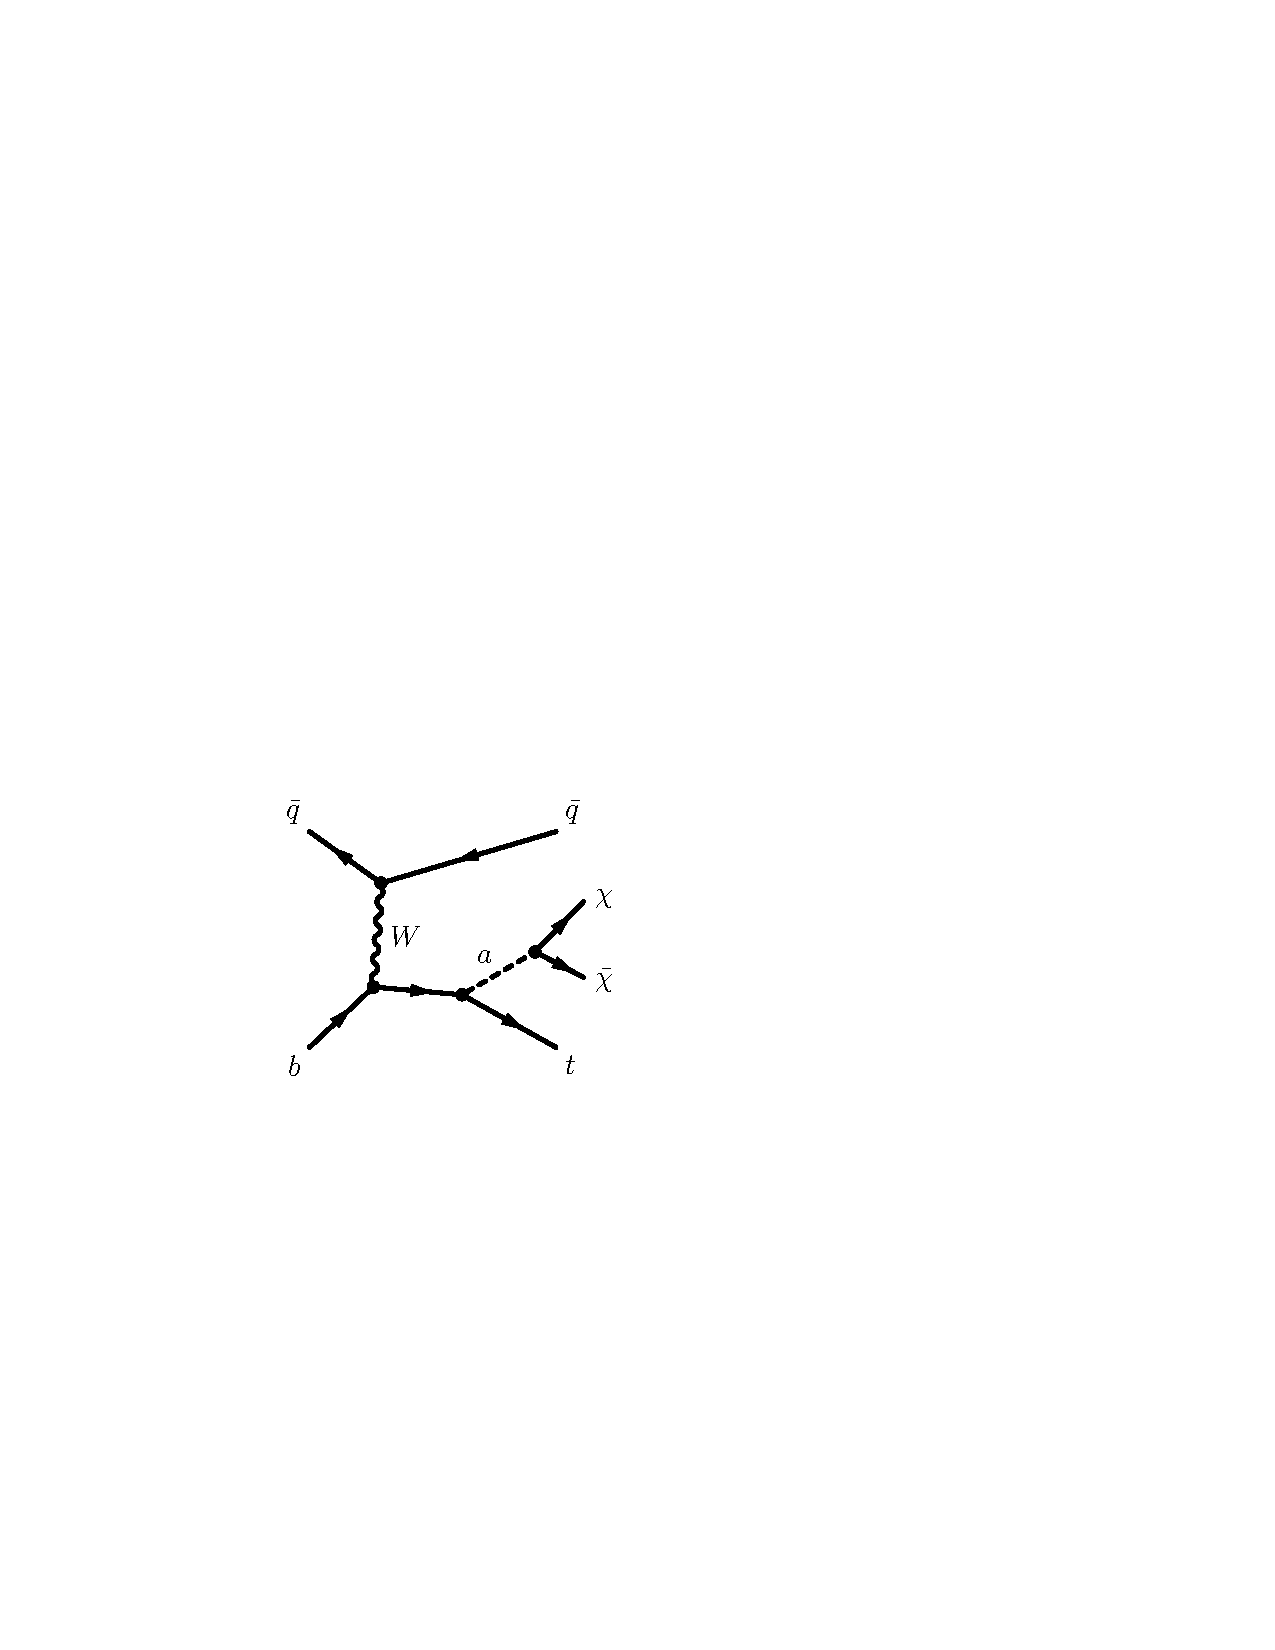
\includegraphics[width=\textwidth]{texinputs/04_grid/figures/DMHF/Pfeyn_tchan_1}
\caption{}
\end{subfigure}
\begin{subfigure}{.23\textwidth}\centering
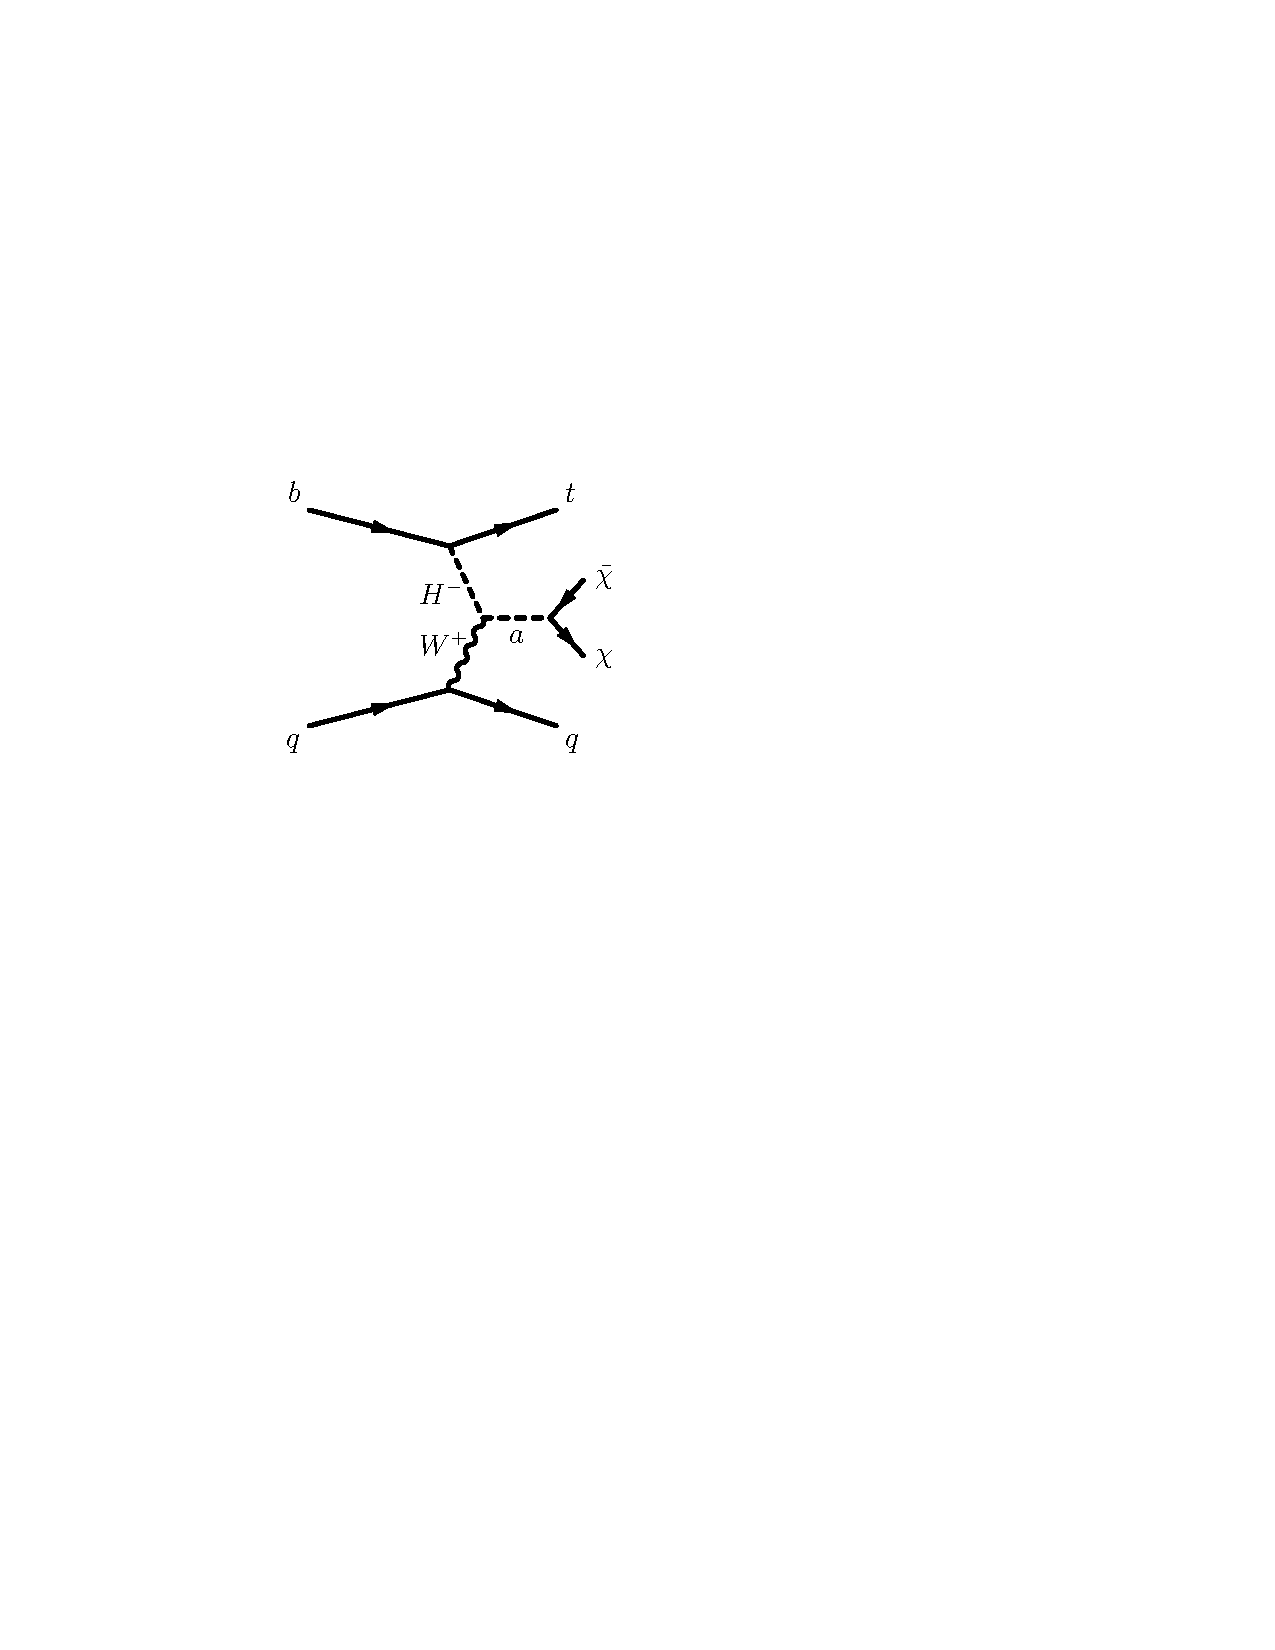
\includegraphics[width=\textwidth]{texinputs/04_grid/figures/DMHF/Pfeyn_tchan_2}
\caption{}
\end{subfigure}
\caption{Representative diagrams for $tW$ and $t$-channel production of DM in association with a single top quark.}
%($pp \rightarrow tj\chi\chi$)}
\label{fig:feyn1}
\end{center}
\end{figure}


Like single top production within the SM, the DM$t$ signature in the model
 receives  three different types of contributions at leading order (LO) in QCD. These are $t$-channel production, $s$-channel production and
associated production together with a $W$ boson ($tW$) (Fig.~\ref{fig:feyn1}).
When the decay $H^{\pm}\rightarrow W^{\pm} a$ is possible, the $H^{\pm}$ is produced on-shell, 
and the cross-section of $pp \rightarrow tW\chi\chi$, 
assuming  $H^{\pm}$ masses of a few hundred \GeV, is around one order of magnitude larger 
than the one for the same process in the simplified model. Moreover the production 
and cascade decay of a resonance yields kinematic signatures
which can be exploited to separate the signal from the SM background. 


Dedicated selections considering one and two lepton final states are
developed to assess the coverage in parameter space for this signature 
at a centre-of-mass energy of  $14$ TeV assuming an integrated
luminosity of 300~fb$^{-1}$ in Ref.~\cite{Pani:2017qyd}. 
Background and signal Monte Carlo simulated
samples are employed for the estimate of the results. The effect of the detector on the kinematic quantities
utilised in the analysis is simulated by applying a Gaussian smearing to the momenta
of  the different reconstructed objects and reconstruction and tagging efficiency factors.
Figure~\ref{DMHF:monotopres} shows the sensitivy reach for two of the
parameter scans proposed in this whitepaper. 
On the top panel the exclusion reach for the $m(a),tan\beta$ plane is
presented, assuming $sin\theta = 0.35$ and $m(A) = m(H^\pm) = m(H) =
500$ GeV. 
%The results are derived from the simulated samples using a
%re-scaling  procedure described in Ref.[IN PREPARATION]
It is possible to observe that for this scenario the sensitivity reach
is comparable to the one from the mono-h signature as presented in
Ref.~\cite{Bauer:2017ota}. On the bottom panel of
Figure~\ref{DMHF:monotopres} the signature's sensitivity to benchmark \#4
 is evaluated for the first time. 

\begin{figure}
\centering
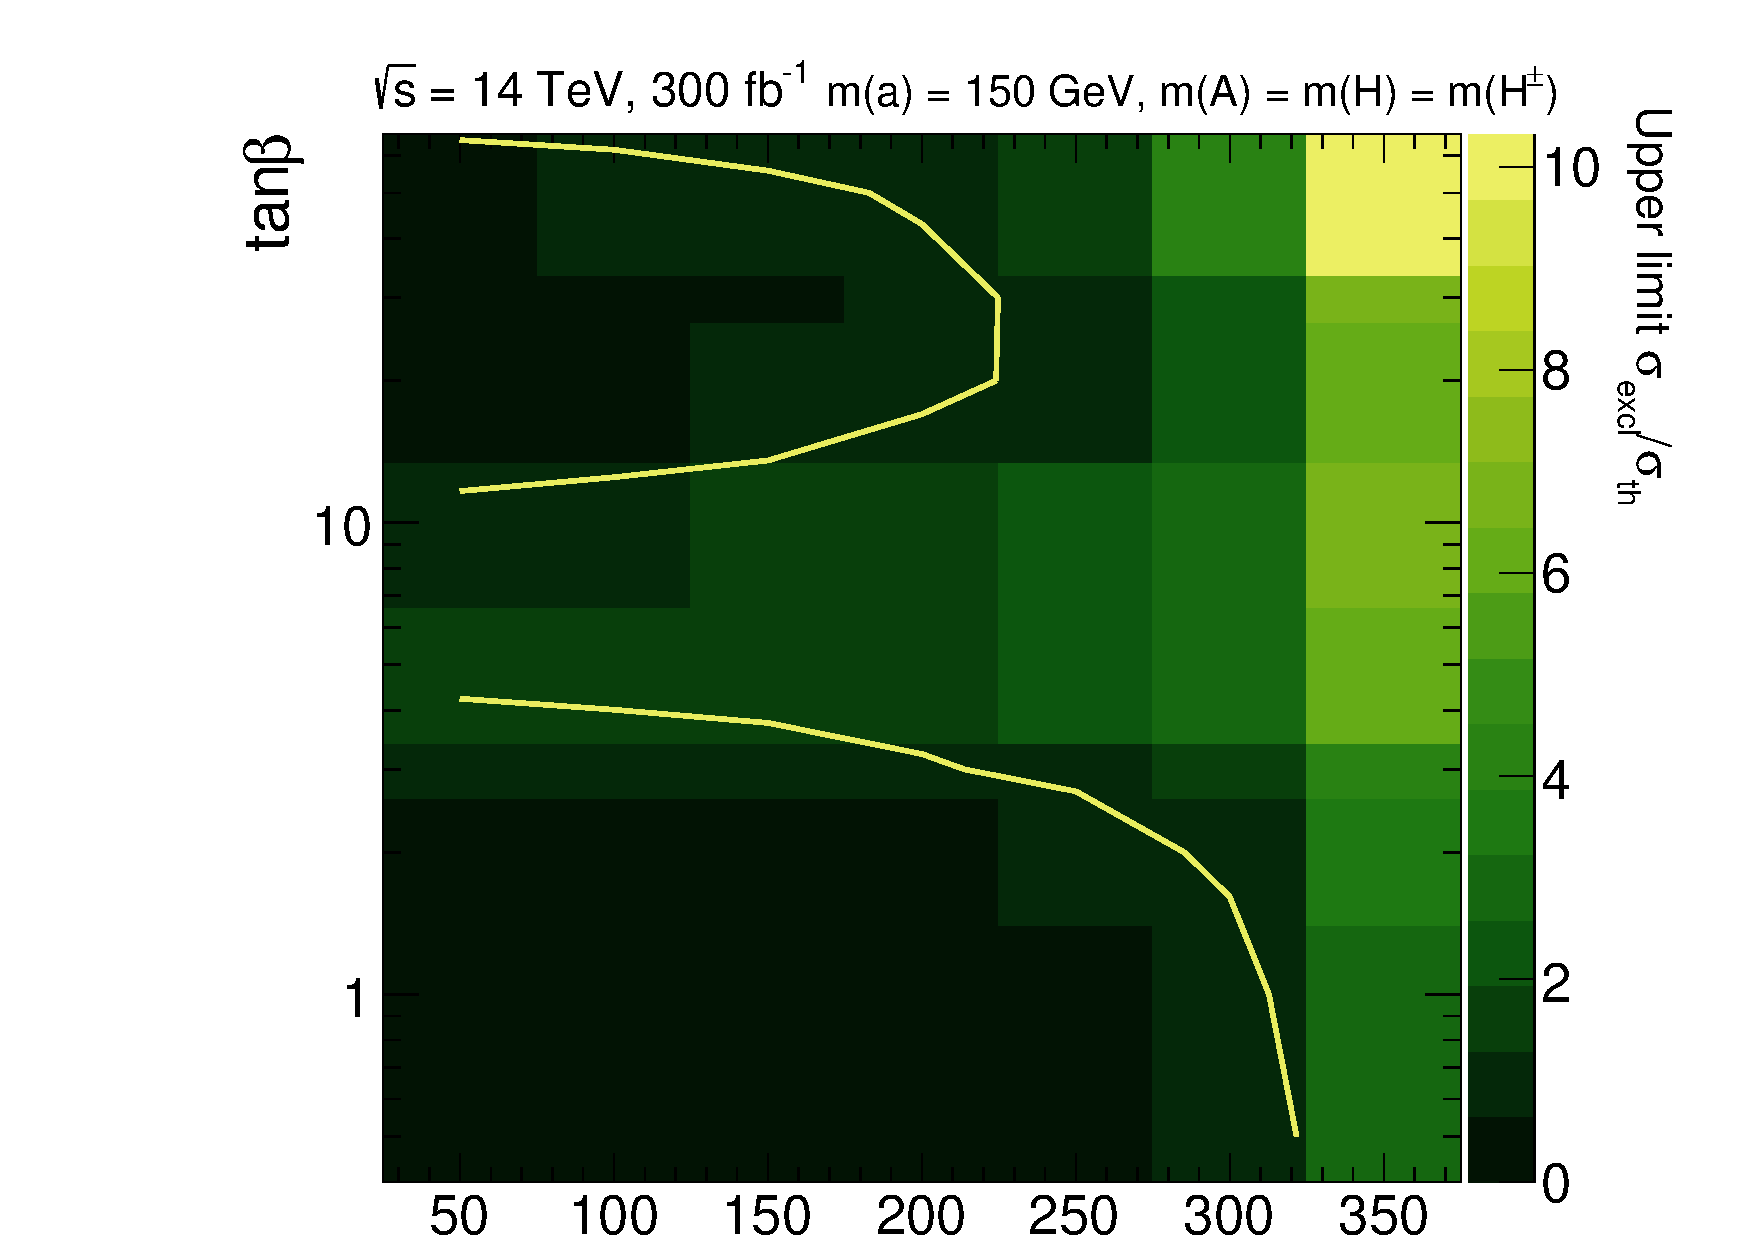
\includegraphics[width=.48\textwidth]{texinputs/04_grid/figures/DMHF/SRrec2l_2DSCAN_a}
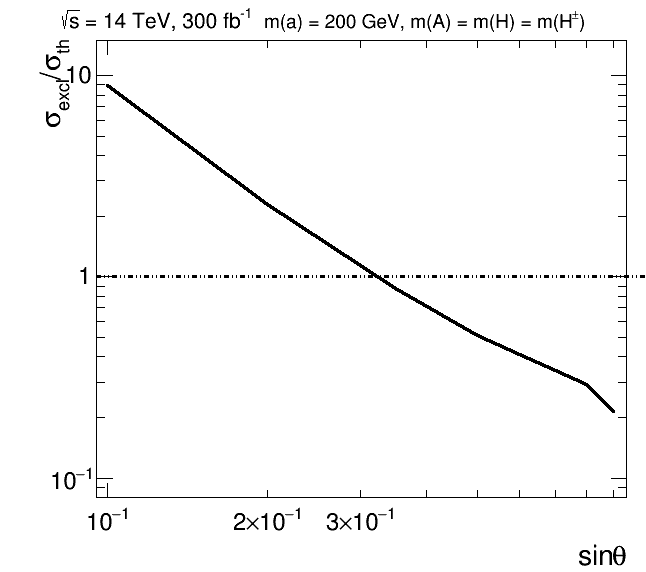
\includegraphics[width=.47\textwidth]{texinputs/04_grid/figures/DMHF/SR2la_ULscan4}
\caption{Exclusion reach for  benchmark \#2 (top) and benchmark \#4 (bottom), 
assuming $sin\theta = 0.35$ and $m(A) = m(H^\pm) = m(H) = 500$ GeV.}
\label{DMHF:monotopres}
\end{figure}


%%%%-----------------------------------------------------------------------------------------
%%%%-----------------------------------------------------------------------------------------
%%%%-----------------------------------------------------------------------------------------
\subsubsection{Uncovered signatures with $tt h+\met$}

As discussed in Section~\ref{sub:hfttrecast}, the production of the
heavy mediator $A$ gives a sizeable contribution to the $tt+\met$  
production cross section in the $2HDM+a$ model. This is also true for
the heavy $H$. When the decay of these mediators into the lightest
pseudoscalar $a$ is allowed, this decay process dominates over the
direct decay into $\chi\chi$. In symmetry with what happens for the
mono-h signature discussed in \cite{Bauer:2017ota}, for certain region
of parameter space the signatures $pp \rightarrow t\bar t A
\rightarrow t \bar t a h$ and $pp \rightarrow t\bar t H
\rightarrow t \bar t a Z$ become sizeable. For the former case, it can
be estimated from Fig. 12(b) of Ref.~\cite{Bauer:2017ota} that for
relatively small $m(A)$ the $pp \rightarrow t\bar t ah$ cross section
can be up to 30\% that of the $pp\rightarrow t \bar t \chi\chi$
process. The interplay between the parameters of the model, and
especially between the heavy higgs masses for these types of final
state render the phenomenology interesting and variegated, as can be
seen for example in the branching ratio study of Fig.~\ref{fig:brAHah}, although
further studies are needed to fully understand the interplay and the
complementarity between these $tth+\met$ channels and the traditional
heavy flavour dark matter searches. 

\begin{figure}
\centering
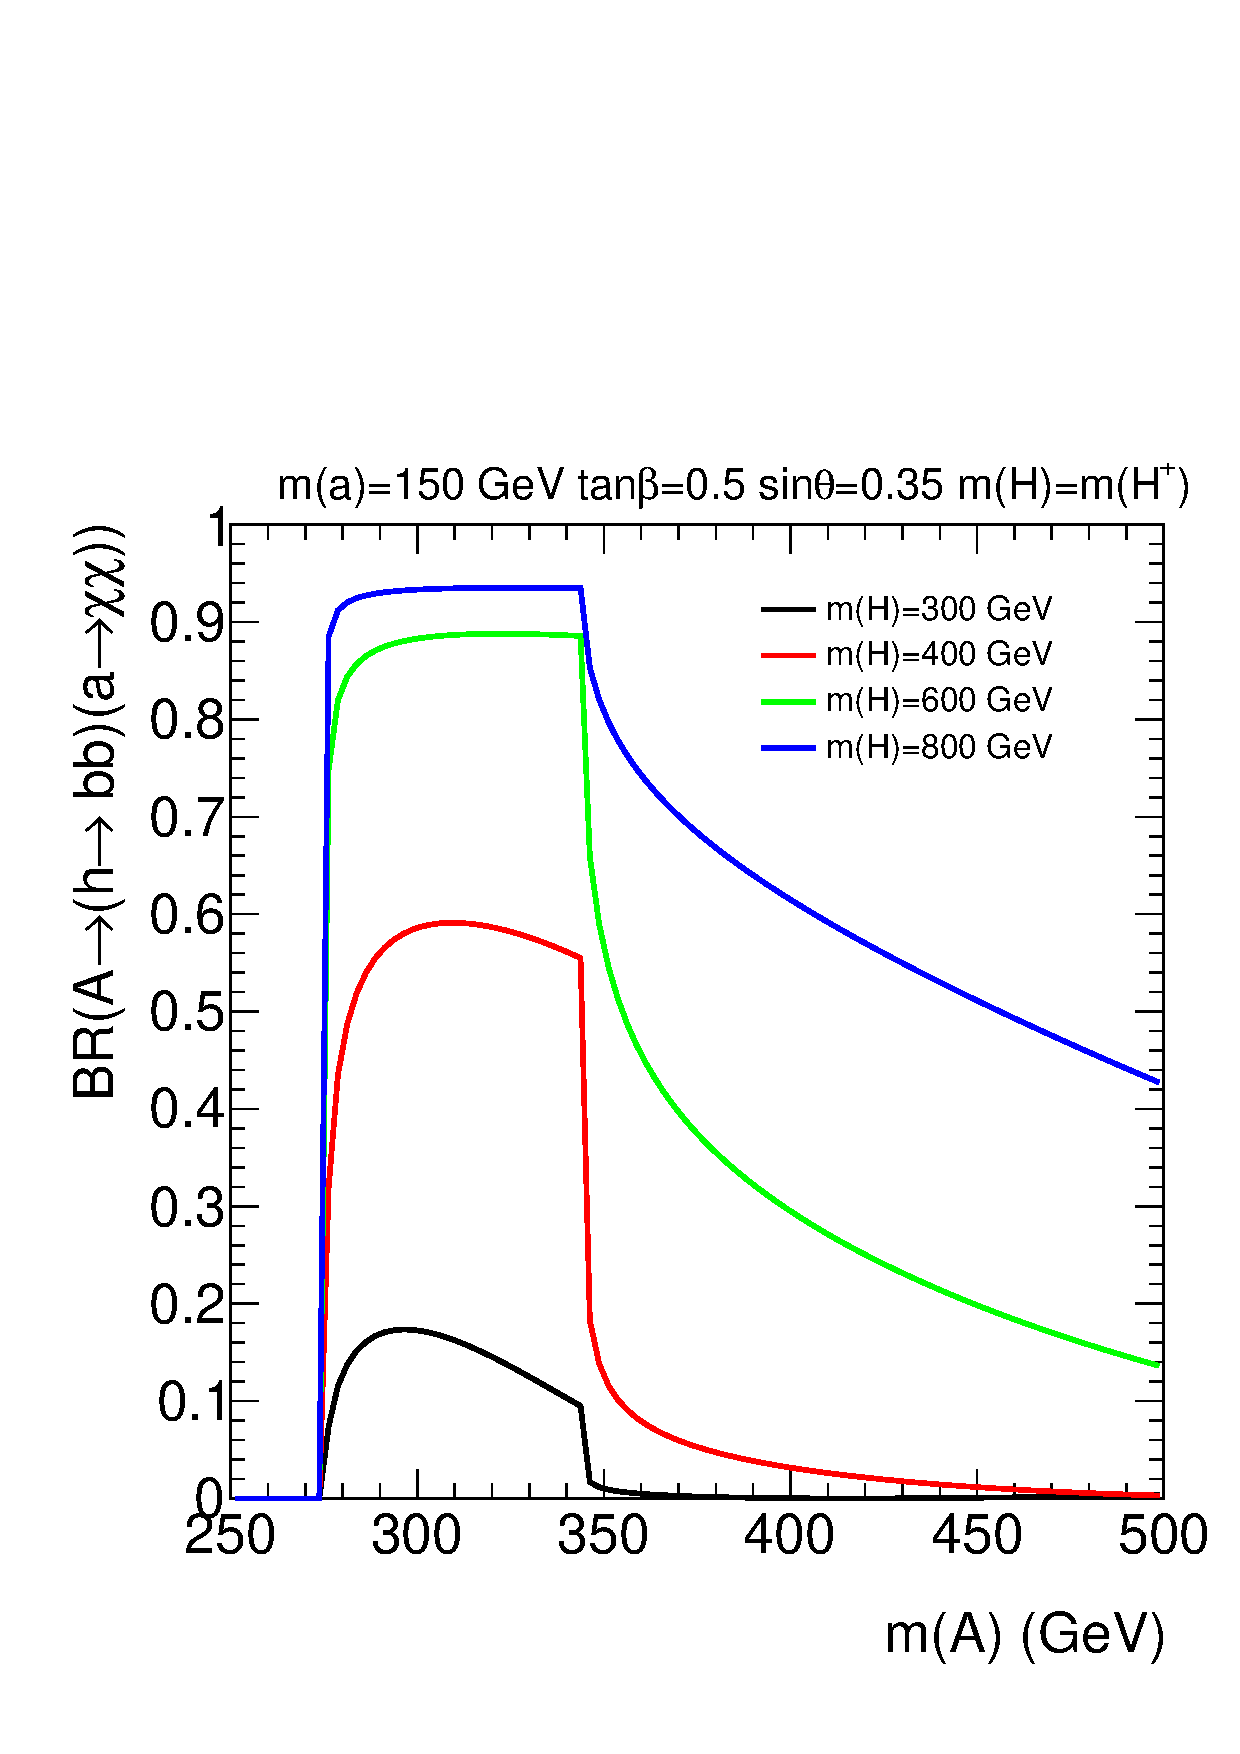
\includegraphics[width=.48\textwidth]{texinputs/04_grid/figures/DMHF//brA}
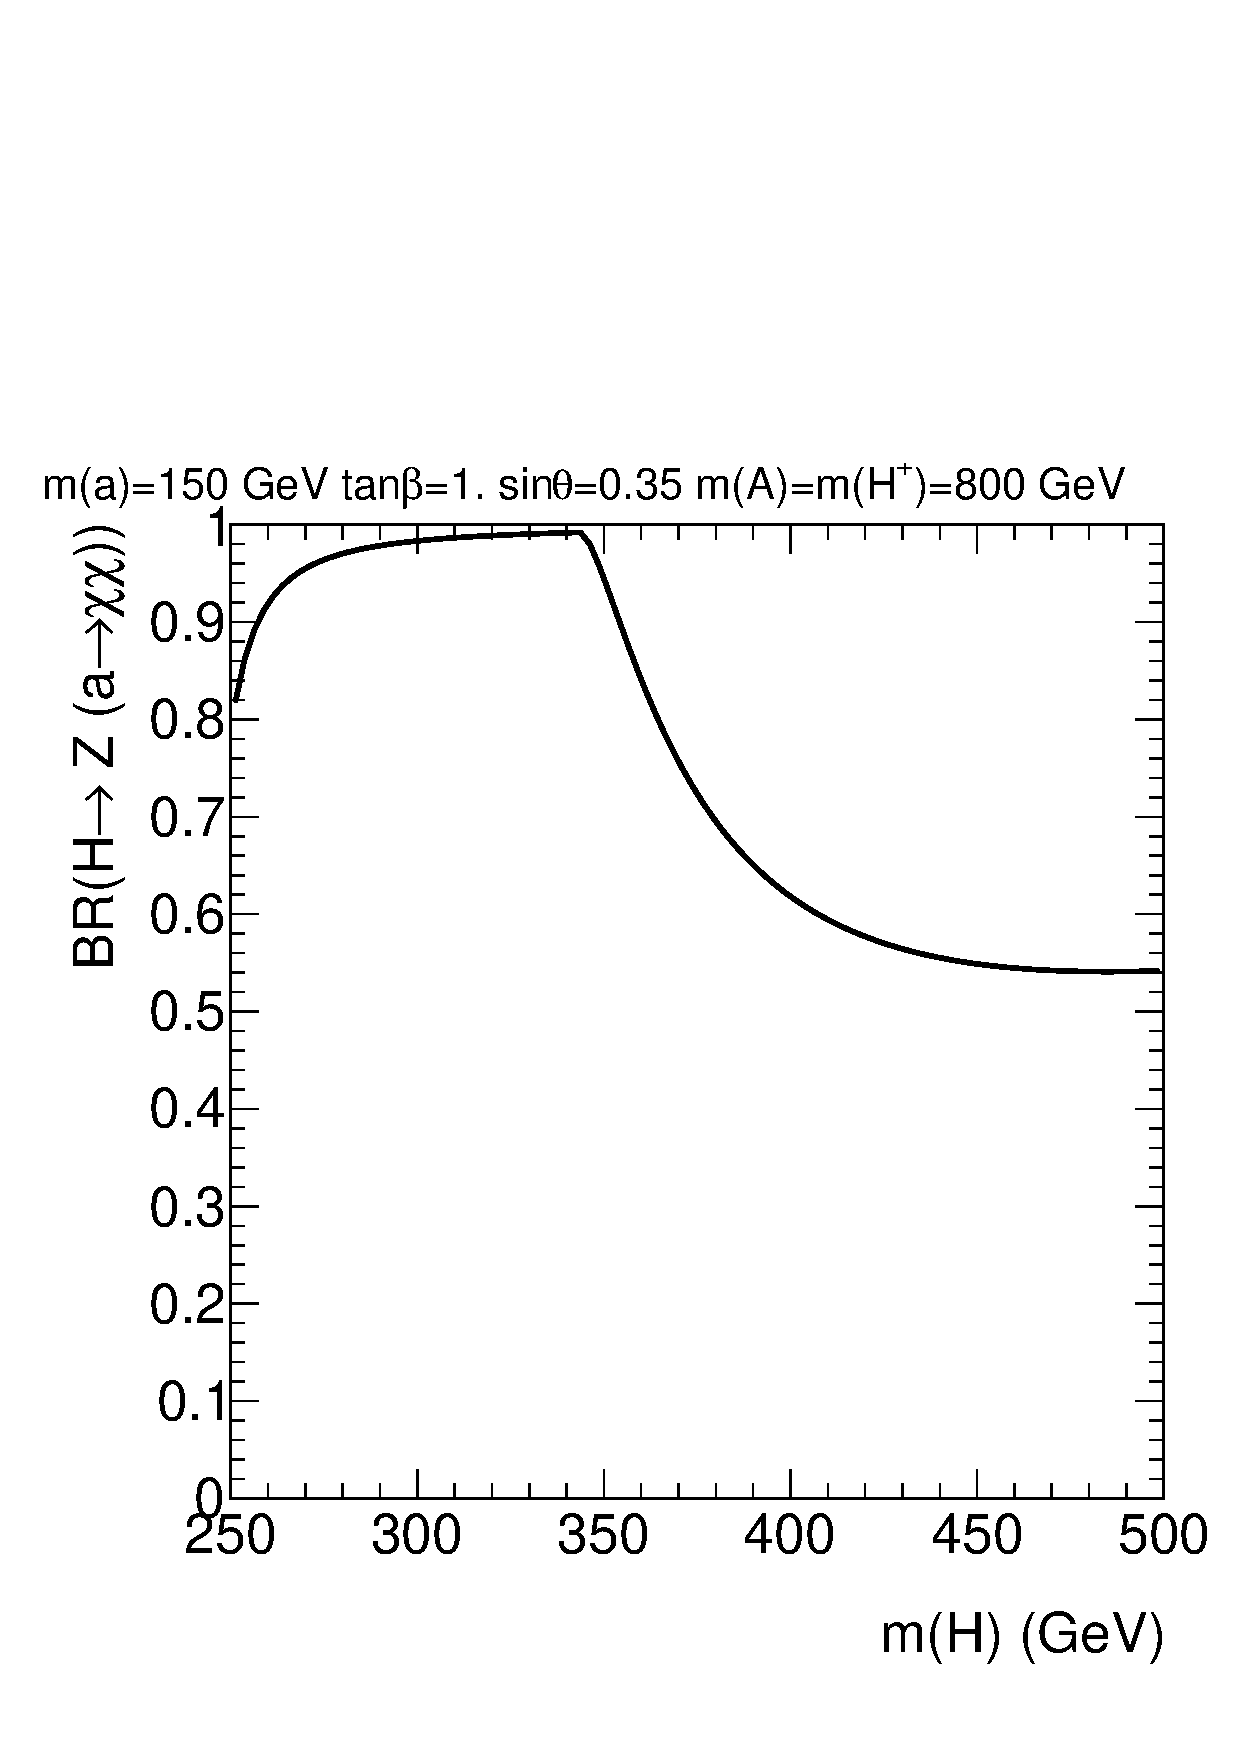
\includegraphics[width=.48\textwidth]{texinputs/04_grid/figures/DMHF//brH}
\caption{Example of the dependence of the $A$ and $H$ branching ratio into $ah$ as a function of some parameters of the 2HDM model.}
\label{fig:brAHah}
\end{figure}
%%%%-----------------------------------------------------------------------------------------

%%%%-----------------------------------------------------------------------------------------

%%%%-----------------------------------------------------------------------------------------
\FloatBarrier
\subsubsection{Top pair resonant searches}
Heavy (pseudo)scalar bosons with $M_{A/H}\ge2\mt$ and $\tanb \sim \mathcal{O}(1)$ decaying dominantly into top-quark pairs can be
searched for by studying the resulting \ttbar\ invariant mass
spectra. However, interference effects between the signal processes
and the SM \ttbar\ production distort the signal shape from a single
peak to a peak-dip structure \cite{Carena:2016npr}. The first search in this challenging decay channel was conducted recently, probing scalar and pseudoscalar masses between 500 and 650\GeV\ in a minimal 2HDM \cite{Aaboud:2017hnm}. A similar kinematic range could be probed if the result were re-interpreted in the context of the \hdma. Interference between
a loop-induced and a tree-level process cannot currently be simulated in \mg. To amend this problem, the same "Higgs\_Effective\_Couplings\_FormFactor"
approach \cite{ttinterfHFF} as adopted in \cite{Aaboud:2017hnm} is implemented in the UFO, replacing the loop production by an 
effective vertex. The predictions of the modified UFO for the case, in which the pseudoscalar mediator does not mix with the heavy pseudoscalar $A$ ($\sinp=0$), i.e. effectively decouples from the 2HDM Higgs sector, are compared to those for the minimal 2HDM. Excellent agreement is found in the invariant mass distributions of $A/H$ decaying into a top pair are shown in Fig.~\ref{fig:ttres_2HDMvs2HDMa}. As examples of how the sensitivity changes as a function of the parameters of the \hdma, the $M_{\ttbar}$ distributions of pseudoscalars decaying into \ttbar\ are presented in Fig~\ref{fig:ttres_2HDM_A}. Larger values of \tanb\ or \sinp\ are expected to yield lower sensitivities to $A\rightarrow\ttbar$ significantly while \ma\ almost only affects the contribution from $a\rightarrow\ttbar$, which becomes sizeable if \ma is close to $2\mt$.
\begin{figure}
\centering
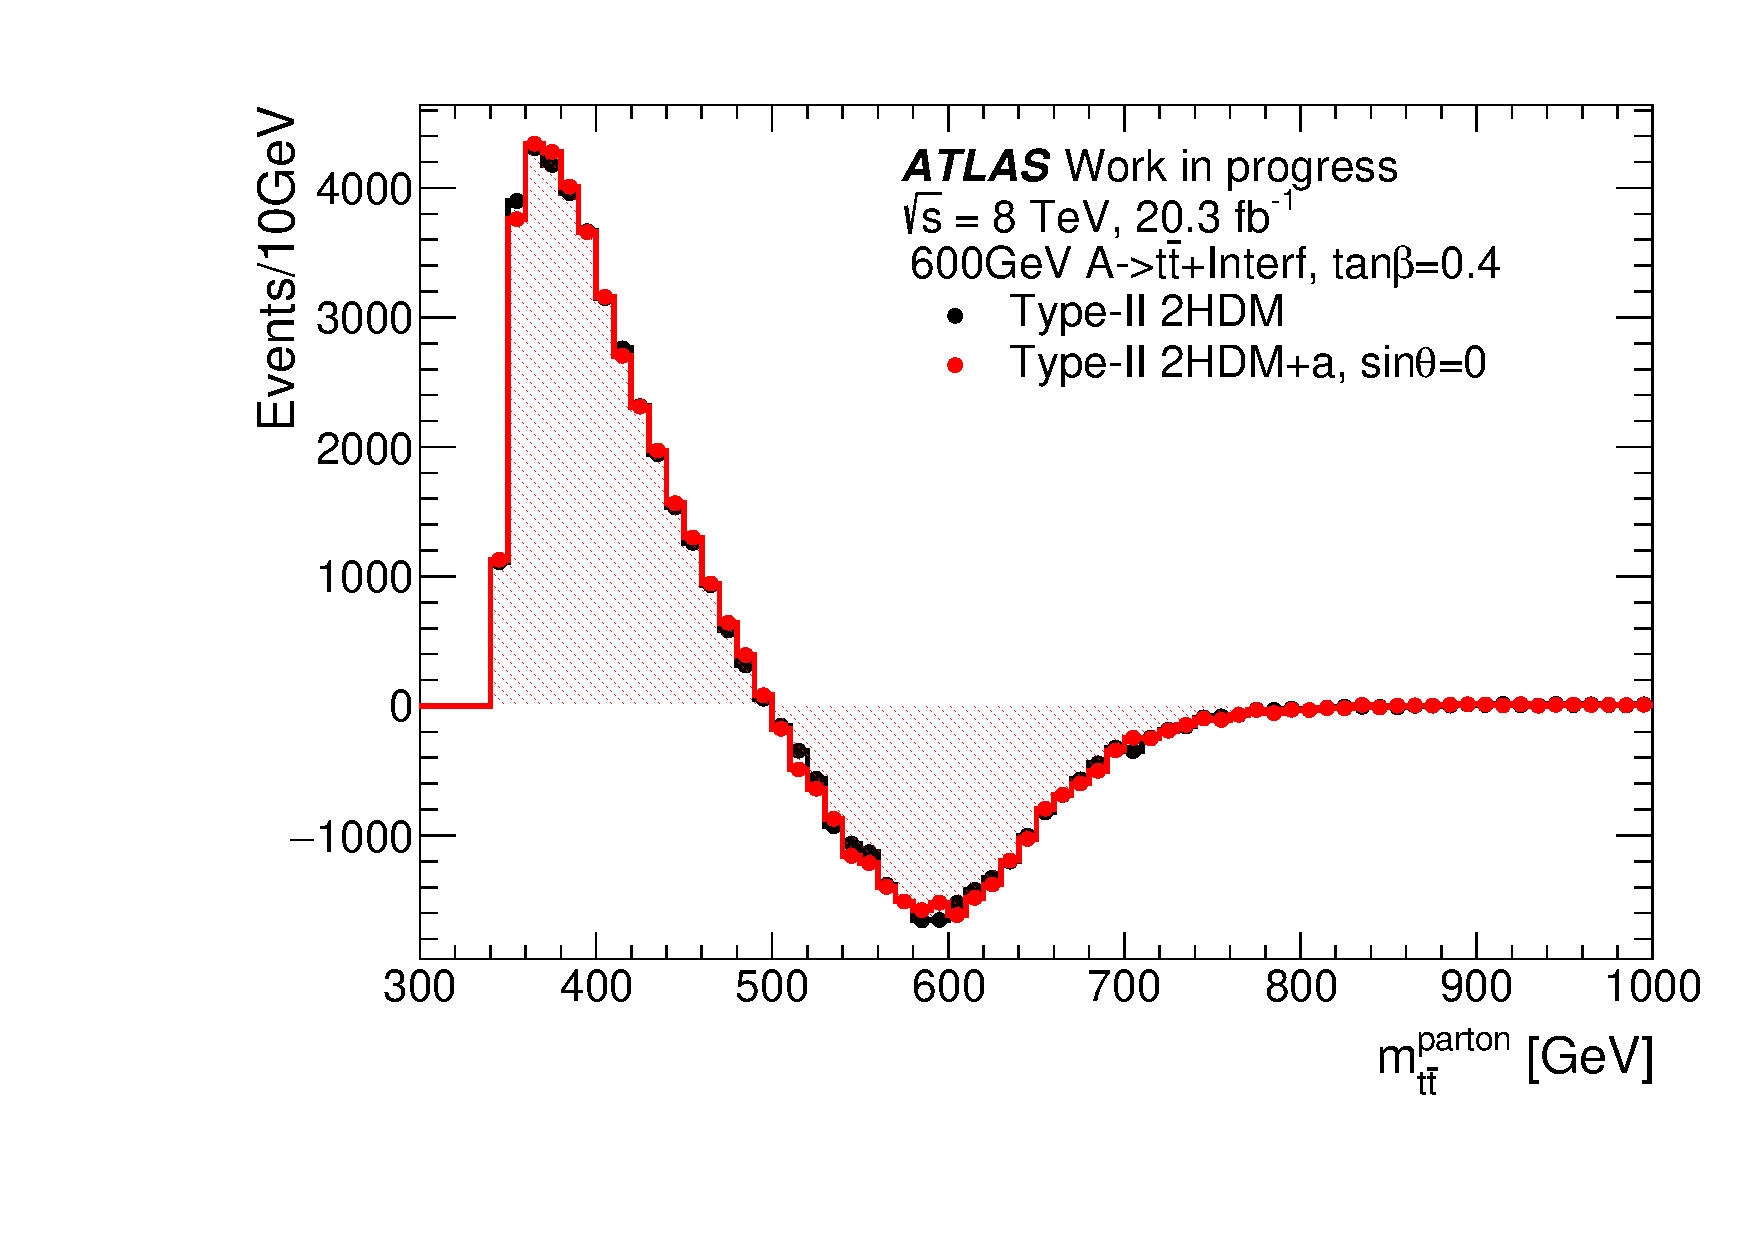
\includegraphics[width=.48\textwidth]{texinputs/04_grid/figures/ttres/ttres_2HDMvs2HDMa_A.pdf}
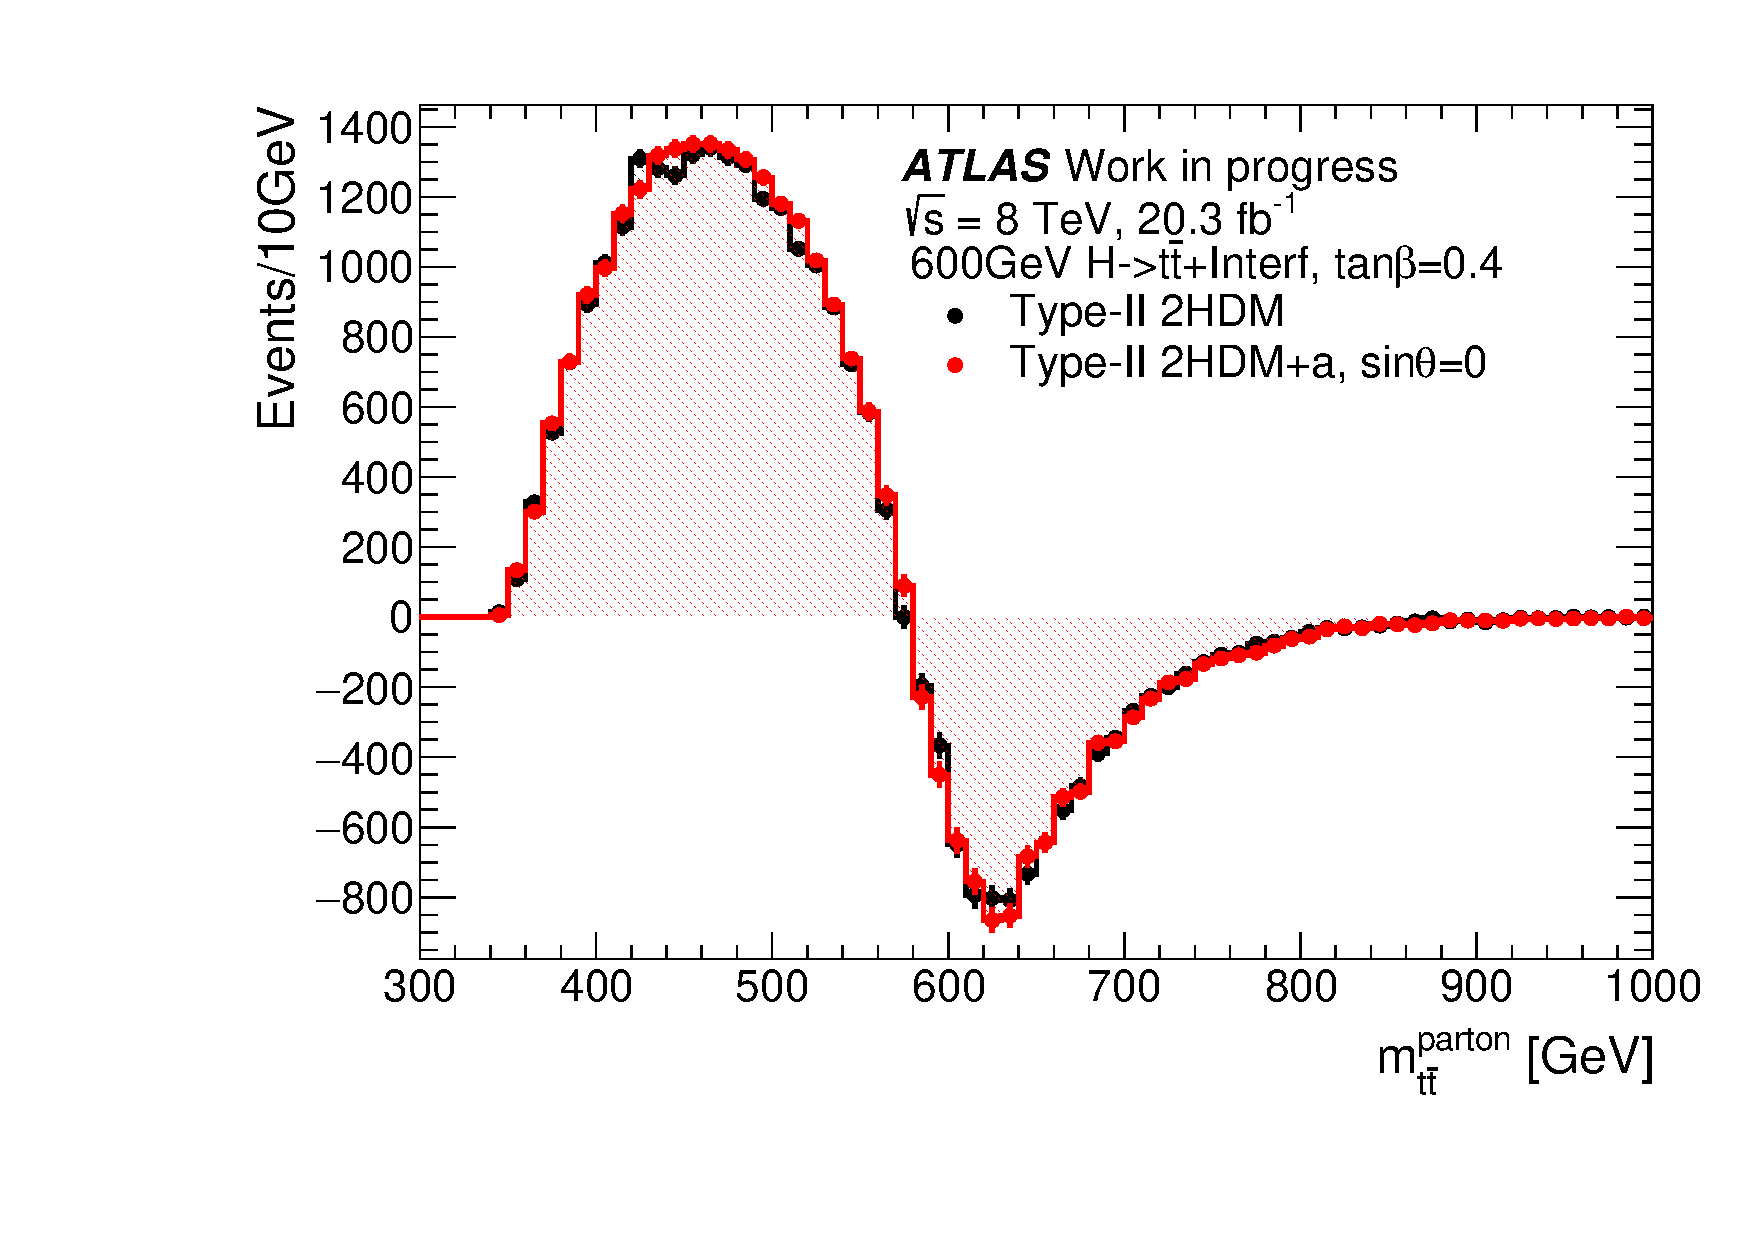
\includegraphics[width=.48\textwidth]{texinputs/04_grid/figures/ttres/ttres_2HDMvs2HDMa_H.pdf}
\caption{$M_{\ttbar}$ distribution of the heavy (pseudo)scalar boson decaying into \ttbar\ with $\mA=\mH=600\GeV, \tanb=0.4$, $\sinp=1/\sqrt{2}$ and $M_a=100\GeV$ in comparison with the one from the generic 2HDM.}
\label{fig:ttres_2HDMvs2HDMa}
\end{figure}

\begin{figure}
\centering
\begin{subfigure}[b]{0.49\textwidth}
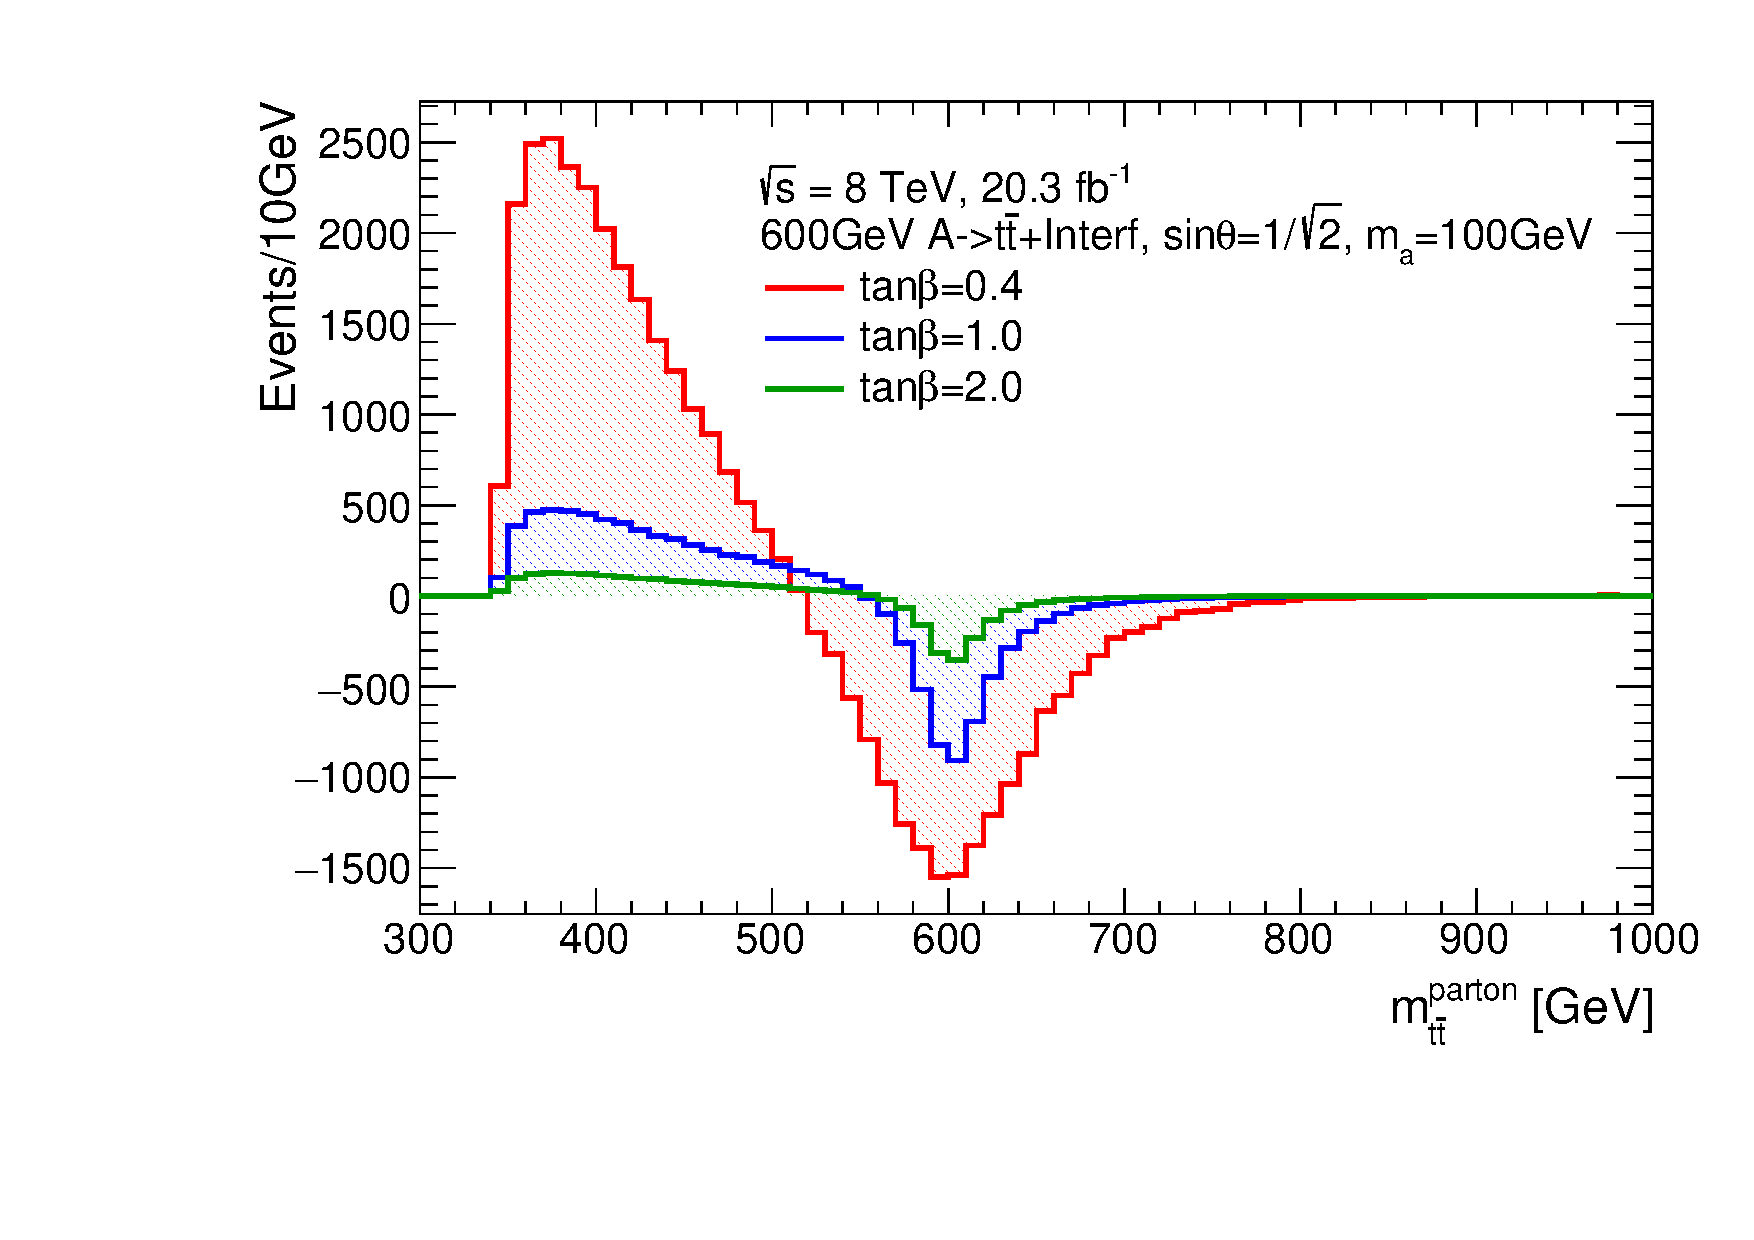
\includegraphics[width=\textwidth]{texinputs/04_grid/figures/ttres/ttres_2HDMa_A_tanb.pdf}
\caption{\tanb dependency with fixed $\sinp=1/\sqrt{2}$ and $\ma=100\GeV$}
\end{subfigure}
\begin{subfigure}[b]{0.49\textwidth}
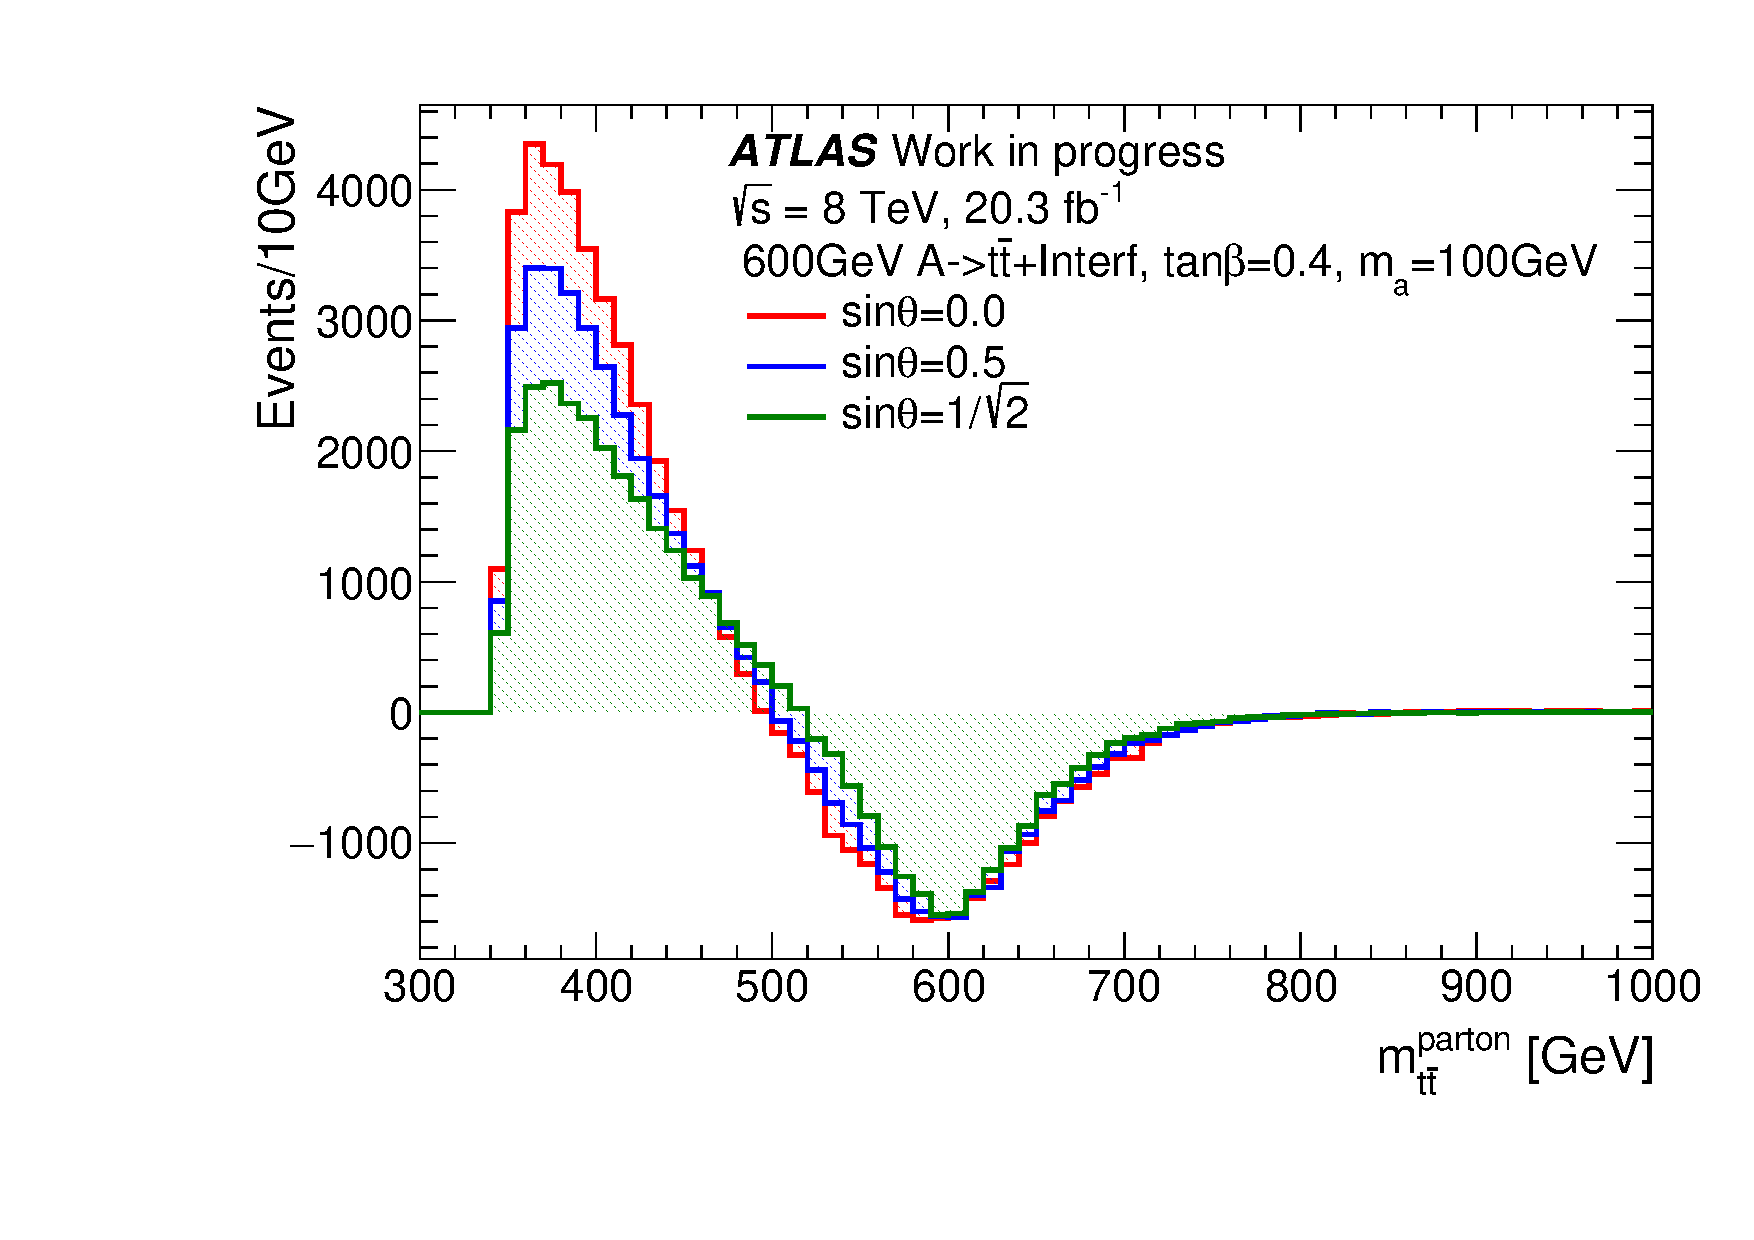
\includegraphics[width=\textwidth]{texinputs/04_grid/figures/ttres/ttres_2HDMa_A_sinp.pdf}
\caption{\sinp dependency with fixed $\tanb=0.4$ and $\ma=100\GeV$}
\end{subfigure}
\begin{subfigure}[b]{0.49\textwidth}
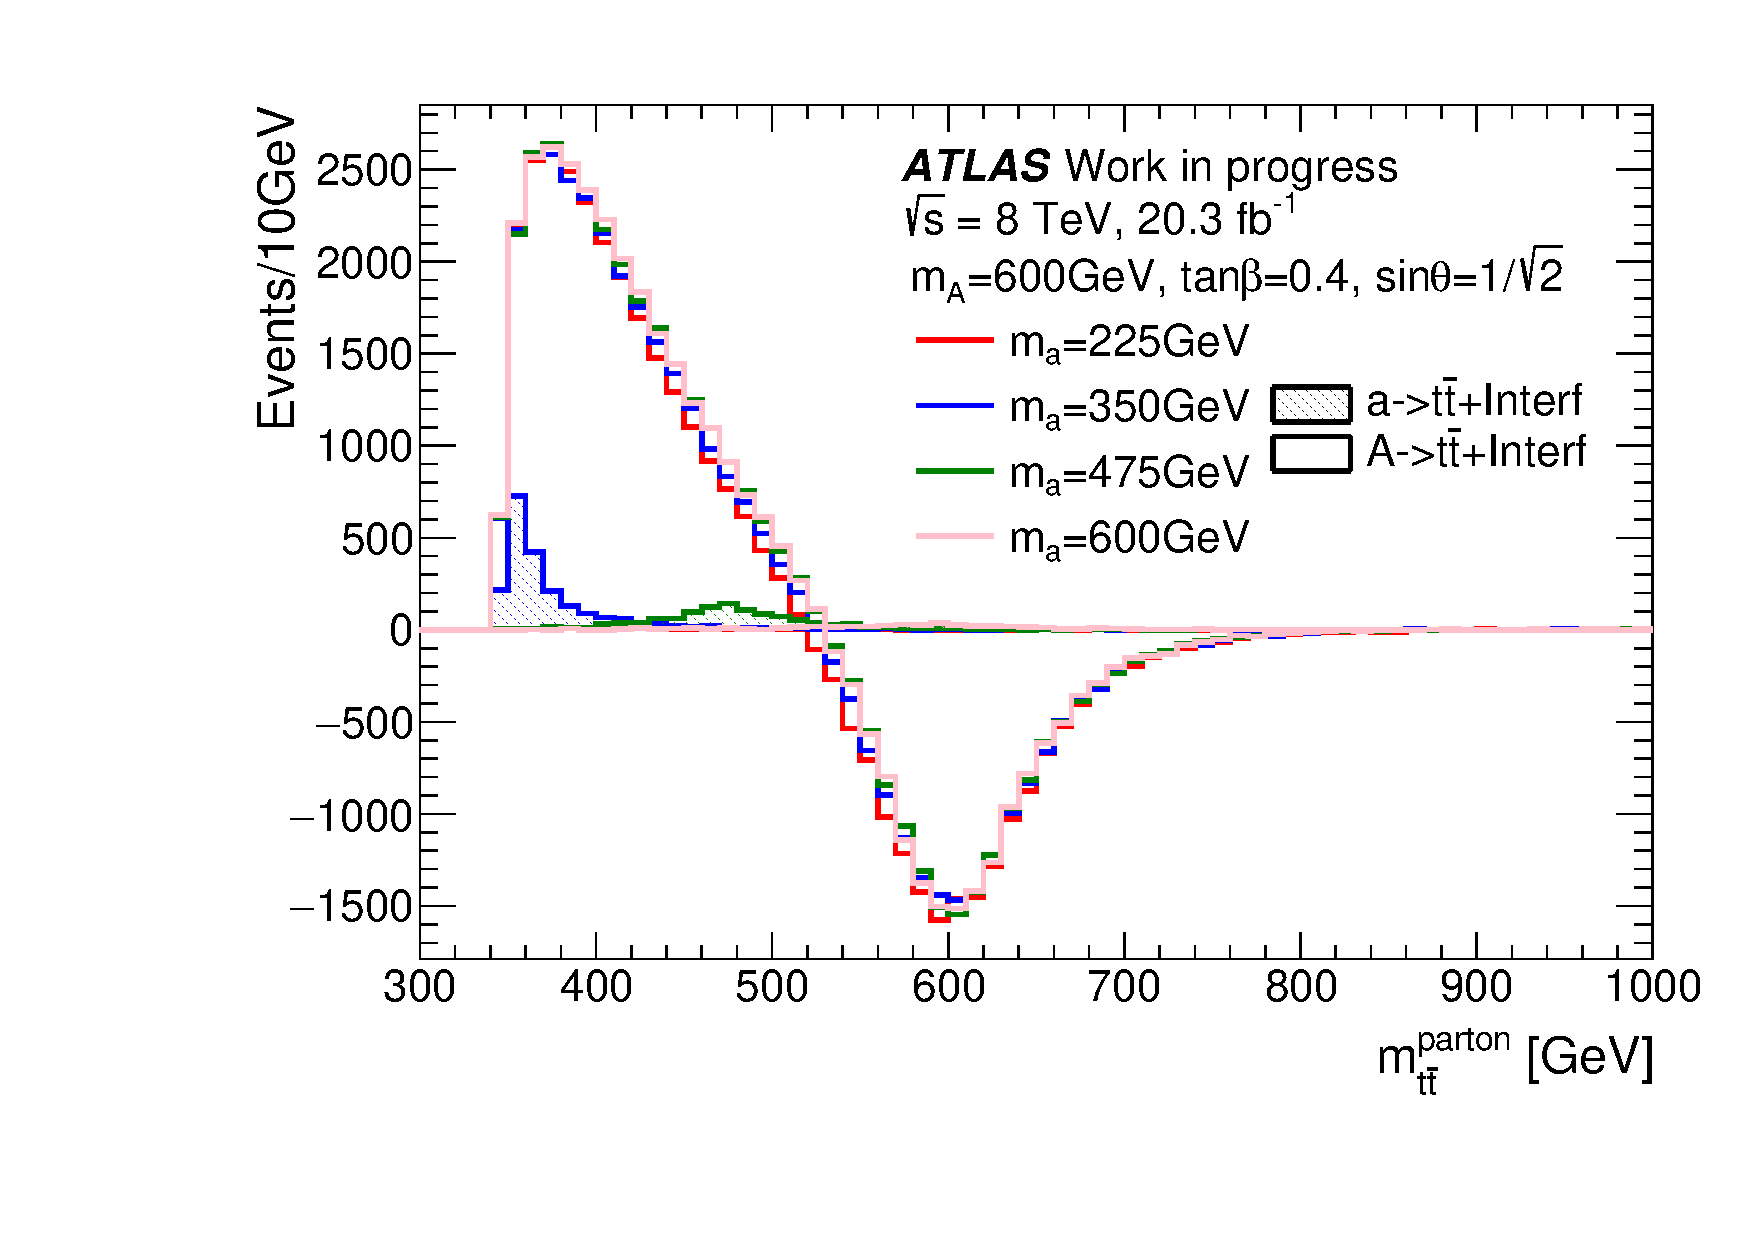
\includegraphics[width=\textwidth]{texinputs/04_grid/figures/ttres/ttres_2HDMa_A_ma.pdf}
\caption{\ma dependency with fixed $\tanb=0.4$ and $\sinp=1/\sqrt{2}$}
\end{subfigure}
\caption{parameter dependency of signal $M_{\ttbar}$ distribution mediated by pseudosalars. The value of \mA is fixed at 600\GeV.}
\label{fig:ttres_2HDM_A}
\end{figure}
\FloatBarrier
%%%%-----------------------------------------------------------------------------------------

%%%%-----------------------------------------------------------------------------------------
%%%%-----------------------------------------------------------------------------------------
\subsubsection{Four tops final states}

The topology involving four top-quarks in the final state is a rare,
yet increasingly important signature, which will gain sensitivity and
attention with the enlargement of the dataset delivered by the LHC.  
In the attempt to perform a first characterisation of this topology,
we have studied the predicted cross-section for the four top final
state of this model for two sets of parameter choices. 

In Figure~\ref{DMHF-4top-scan1} we present the four top cross section
for the parameter choices of benchmark \#2, for an intermediate choice
of mass of the light pseudoscalar ($m(a) = 400$ GeV), as a function of
$tan\beta$. The total four-top production cross section, which
accounts for both SM and new physics (NP) contributions and is indicated
as $|SM+NP|^2$ in the legend, is compared with the production cross
section contributions separately due to SM and NP terms. 
This is achieved technically by setting a requirement on the number of
QCD and QED vertices in madgraph, as indicated in Table~\ref{tab-dmhf-4tops}.
Furthermore, the different contributions from on-shell production of
each CP-odd and CP-even mediators associated with a top pair and
decaying into a top pair is indicated. The dominant contribution is
driven by the on-shell production of $A$ and $H$ for all choices of
$tan\beta$ in this benchmark. 
In the lower panel of Figure~\ref{DMHF-4top-scan1}, the effect of the
interference term between the 2HDM+a and the SM is assessed, and is
found to have an impact almost always smaller than 5\% on the
inclusive cross-section. \textbf{Checking whether true for some
fiducial cuts, would be important to add statement or clarify that is
is not fully conclusive as it is only inclusive.}

In Figure~\ref{DMHF-4top-scan2} we present instead the cross-section
study for the parameter choices of benchmark \#3b, for $sin\theta
= \frac{1}{\sqrt{2}}$ and as a function of the light pseudoscalar mass. 
Very interestingly, for this parameter choices the cross-section is
quite independent of $m(a)$. As it can
be observed from the on-shell contribution breakdown, at the
low-end of the mass spectrum the $\ttbar+a$ production dominates, with a
peak at $400$ GeV due to the competition between
$a\rightarrow \chi\chi$ and $a\rightarrow \ttbar$ and the natural
decreasing of the cross section with the increase of $m(a)$.  The contribution of
$\ttbar+H$ and $\ttbar+A$ processes compensates the latter effect in
the higher end of the mass-spectrum, with the turn on starting around
$800$ GeV due to the competition between $A/H\rightarrow\ttbar$ and
cascade decays of the heavy higgses into the light pseudoscalar
mediator ($A\rightarrow ah/H\rightarrow aZ$). 
The little bump at 1 TeV is due to interference effects between the
three higgs mediators, which are all set to the
same mass for this parameter choice.  
The inclusive production cross-section of the 2HDM+a
model is also compared with the one obtained by the DMSimp pseudoscalar
implementation. Furthremore, as for the previous benchmark,  the impact of the SM interference
term on the inclusive cross-section is found to be very small
($<2\%$), except for $m(a)$ values close to the top theshold. 


\begin{table}
\begin{tabular}{ccm{50mm}}
\toprule
{\sc Madgraph} rule & Legend symbol & Details \\\midrule
\verb| p p > t t~ t t~ / a z h1 QED<=2|& $|SM+NP|^2$ & Four-top
production including both SM and NP contributions and their
interference. \\\midrule
\verb| p p > t t~ t t~ / a z h1 QCD<=2|& $|NP|^2$ & Four-top
production from NP processes, including interference terms among
$A,H,a$. \\\midrule
\verb| p p > t t~ t t~ / a z h1 QED<=0|& $|SM|^2$ & Four-top SM
production.\\
\bottomrule
\end{tabular}
\caption{Description of the specific MADGRAPH settings used to derive
the different curves of Figs~\ref{DMHF-4top-scan1}~and~\ref{DMHF-4top-scan2}.}
\label{tab-dmhf-4tops}
\end{table}

\begin{figure}
\centering
\begin{subfigure}[b]{0.8\textwidth}
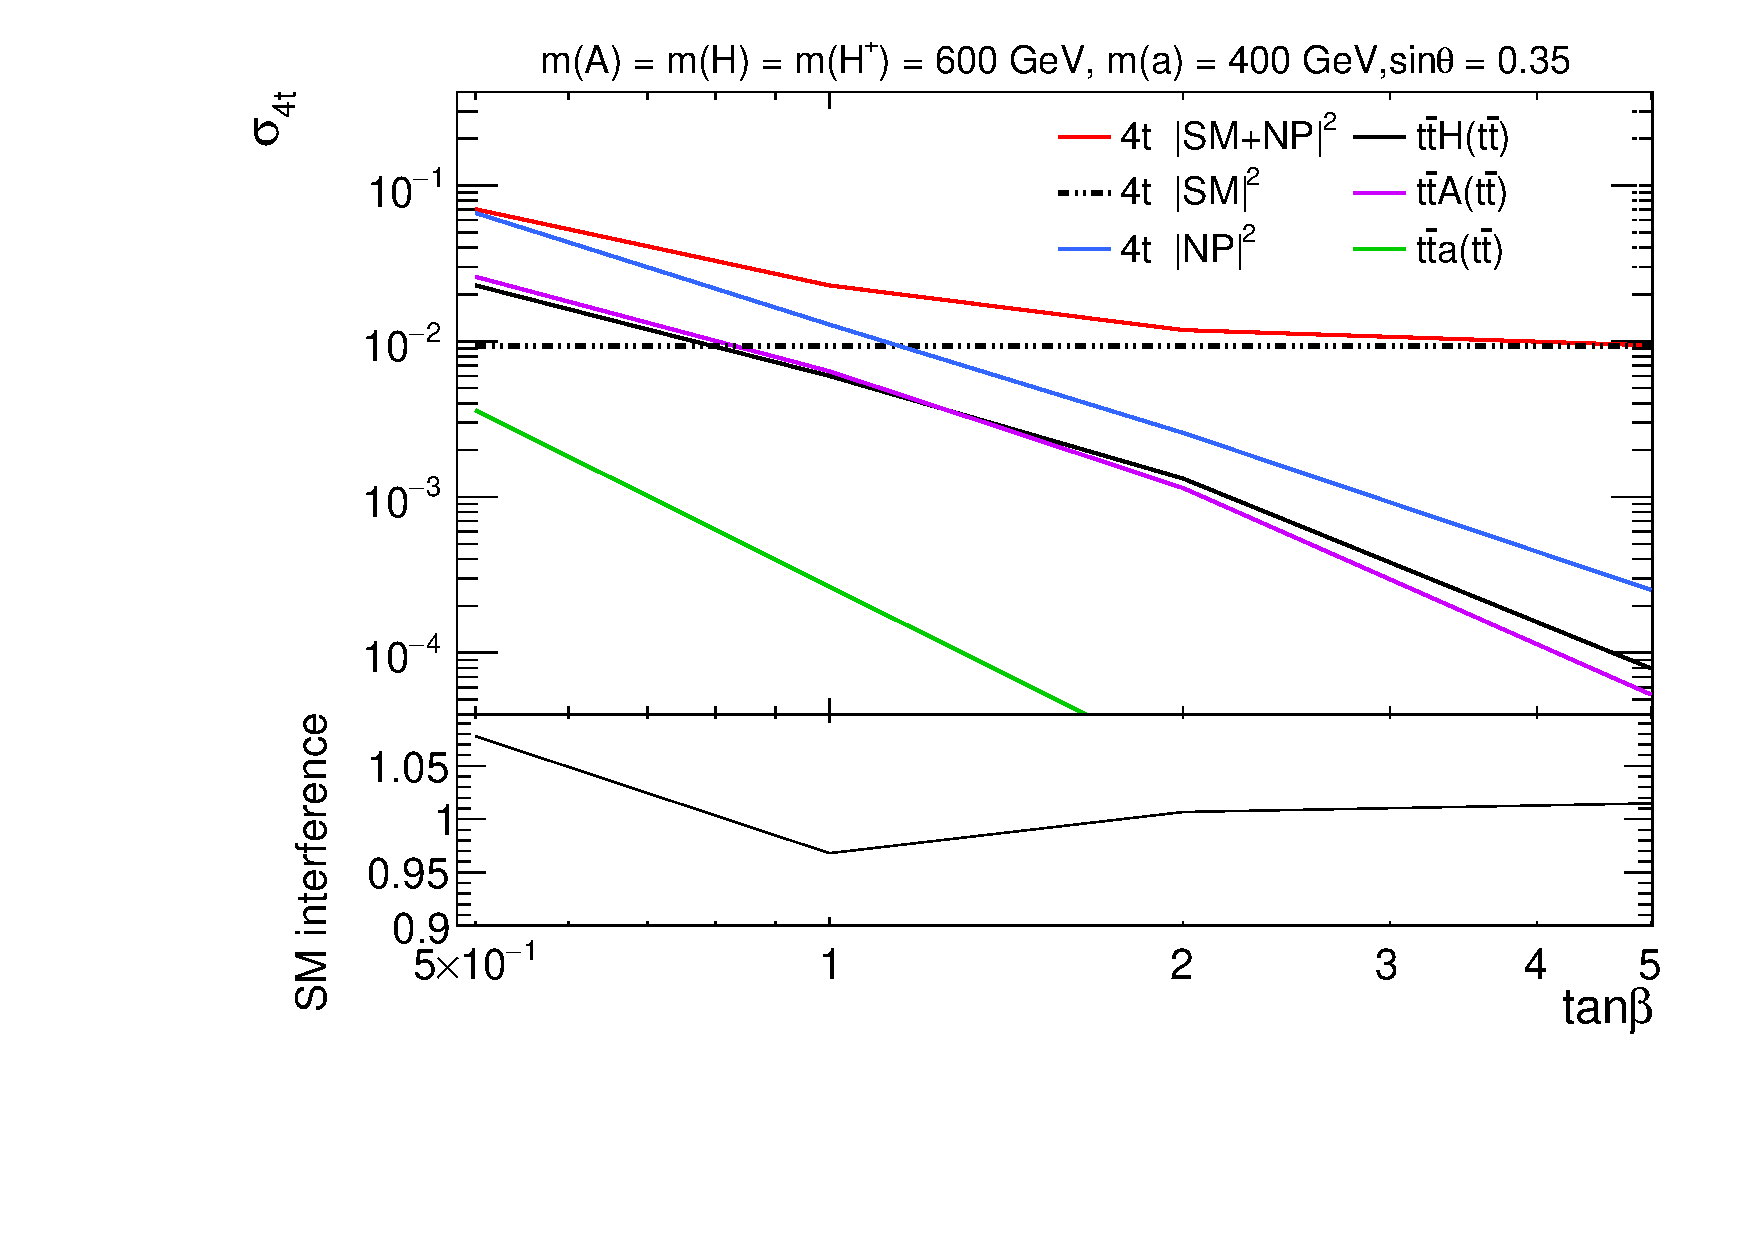
\includegraphics[width=\textwidth]{texinputs/04_grid/figures/DMHF/4tops/WHP_final_tbscan.pdf}
\caption{}
\label{DMHF-4top-scan1}
\end{subfigure}
\begin{subfigure}[b]{0.8\textwidth}
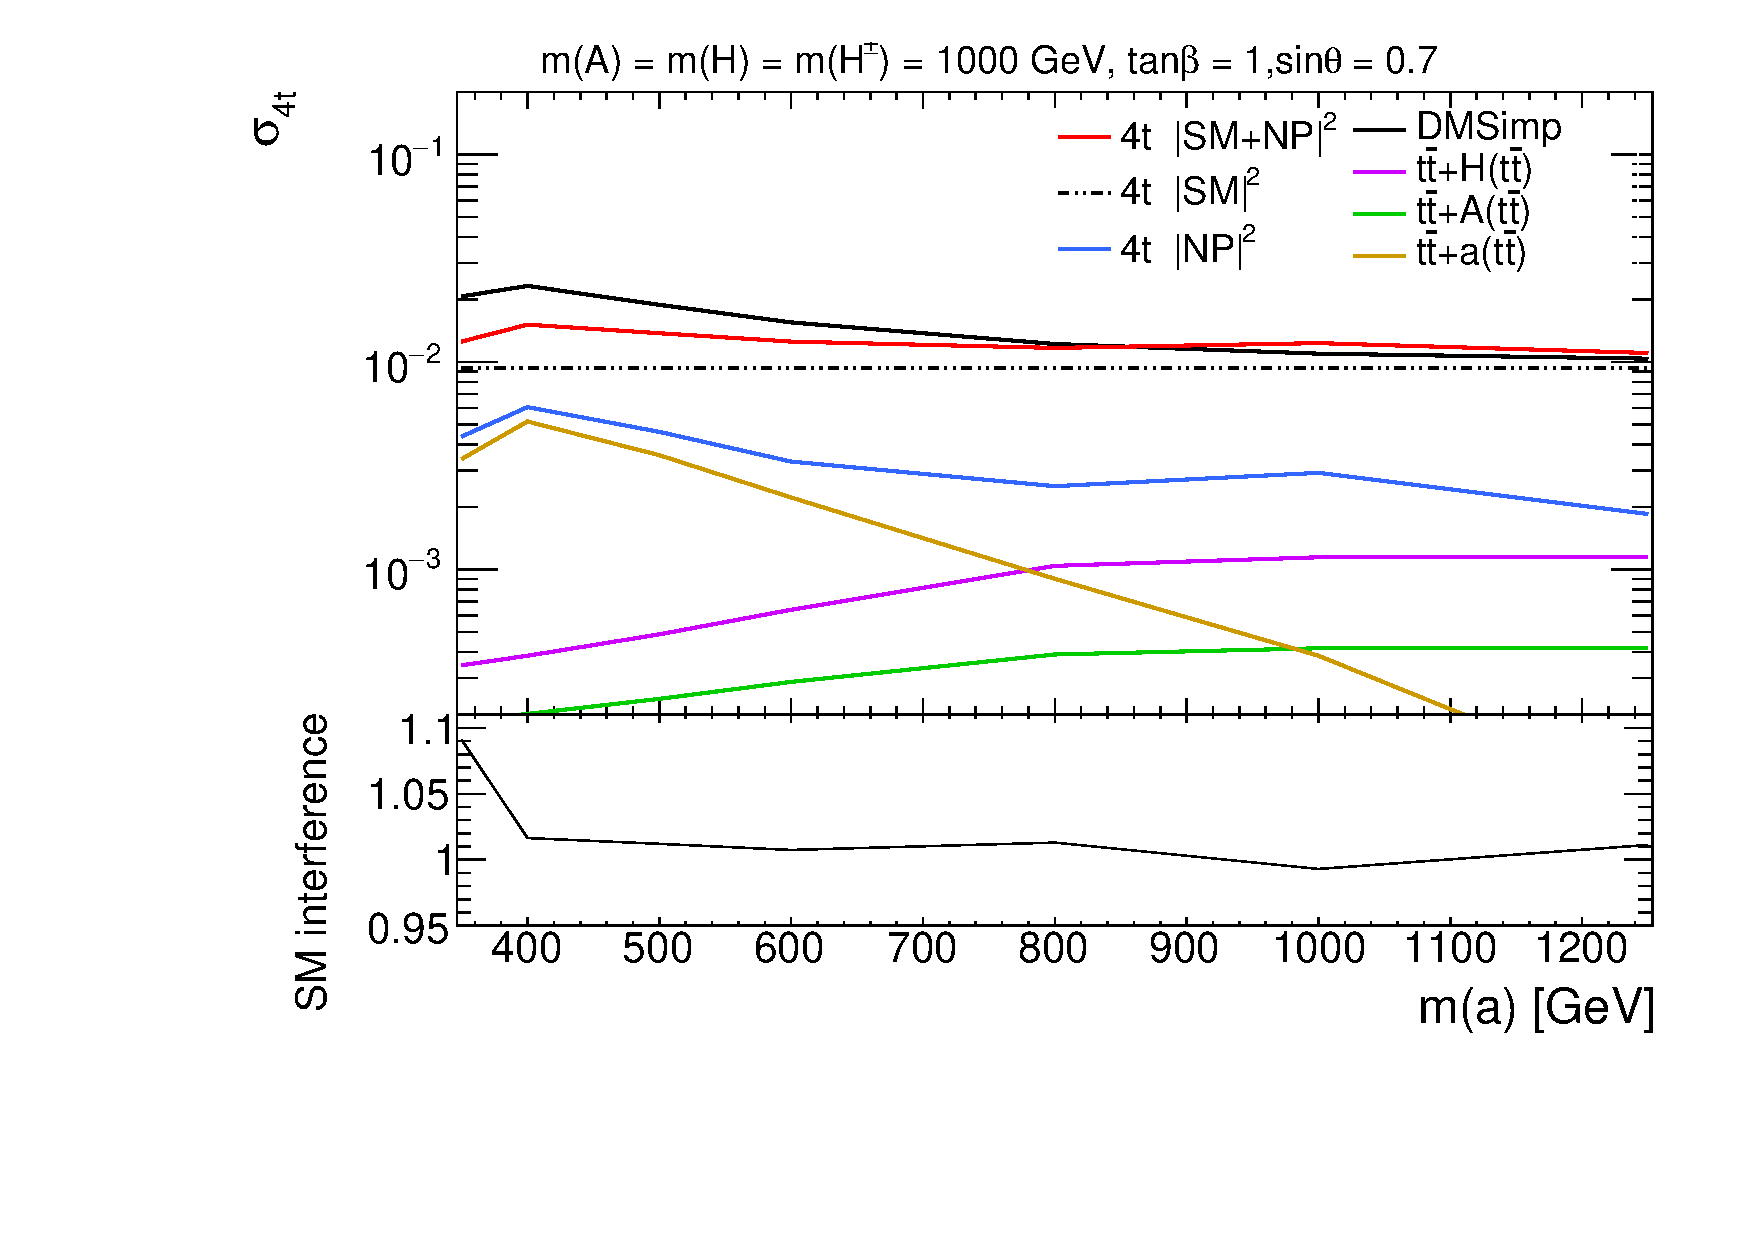
\includegraphics[width=\textwidth]{texinputs/04_grid/figures/DMHF/4tops/WHP_final_mascan.pdf}
\caption{}
\label{DMHF-4top-scan2}
\end{subfigure}
\caption{Four-top cross section study for a subset of the parameter
space of benchmark \#2 (top) and \#3 (bottom). The different Standard
Model (SM) and New Physics (NP) contributions with and without
interference and the breakdown in terms of on-shell mediator
production is presented, following the notation of Table~\ref{tab-dmhf-4tops}. }
\end{figure}


\subsubsection{2HDM+scalar sensitivity studies}

The sensitivity of the tt+\met all-hadronic signature~\ref{Aaboud:2018hf}
to the Type-II model with two Higgs doublets plus a 
scalar portal to dark matter $S_1$ described in~\ref{Bell:2016ekl} has been investigated.
The signature has been chosen as is the one providing the best sensitivity across the majority of the 
mass range for $S_1$ which is most difficult to address. 

The choice of the parameters for this model largely reflects that of the $2HDM+p$ model.
In particular, the masses of the heavier scalar $S_2$ and the masses of the charged Higgs and the CP-odd
scalar have been set to 600 GeV. The value of the mixing angle has been set to $\cos{\theta}=0.35$. 
The mass of the light scalar $S_1$ is scanned between $200$ and $340$ GeV, and $\tan\beta$ is scanned 
between 0.2 and 1. Across the whole $\tan\beta$ and mass range considered the widths of both the light and the heavy 
scalars do not exceed $15\%$ of the mass of the corresponding particle. 

The procedure to extract the results follows closely the procedure described in Sec.~\ref{subsub:hfttrecast}, 
but with the light and heavy pseudo-scalars a and A replaced by the light and heavy scalars
 $S_1$ and $S_2$, respectively.
The formula to rescale the results of the acceptance is therefore turned into:

\begin{equation}
Acc_{2HDM}(m(S_1),M(S_2))=\frac{\sigma_{S_1} \times Acc_{DMSIMP}(m(S_{1}))+
\sigma_{S_2} \times Acc_{DMSIMP}(m(S_{2}))}{\sigma_{S_1}+\sigma_{S_2}}
\label{rewS}
\end{equation}


The validity of this re-scaling has been validated by comparing the acceptance 
to the simplified models to the acceptance to the $2HDM+S_1$ models, before and 
after applying the rescaling of Eq.~\ref{rewS}. The results are shown if Fig.~\ref{fig:rescS1} across the whole
mass range for the light scalar $S_1$ considered, for the minimum and maximum values of 
$\tan\beta$ taken into account. 
It has to be noted that the acceptance to simplified models and $2HDM+S_1$ is very similar even 
before applying the rescaling of Eq.~\ref{rewS}.
This is due to the fact that the ratio between the cross-section of $S_2$ and the cross-section of $S_1$
becomes appreciable (i.e. above sub-percent level) only for models with $m(S_1)>300$ GeV
 and $\tan\beta > 0.4$.\\

\begin{figure}
  \centering
  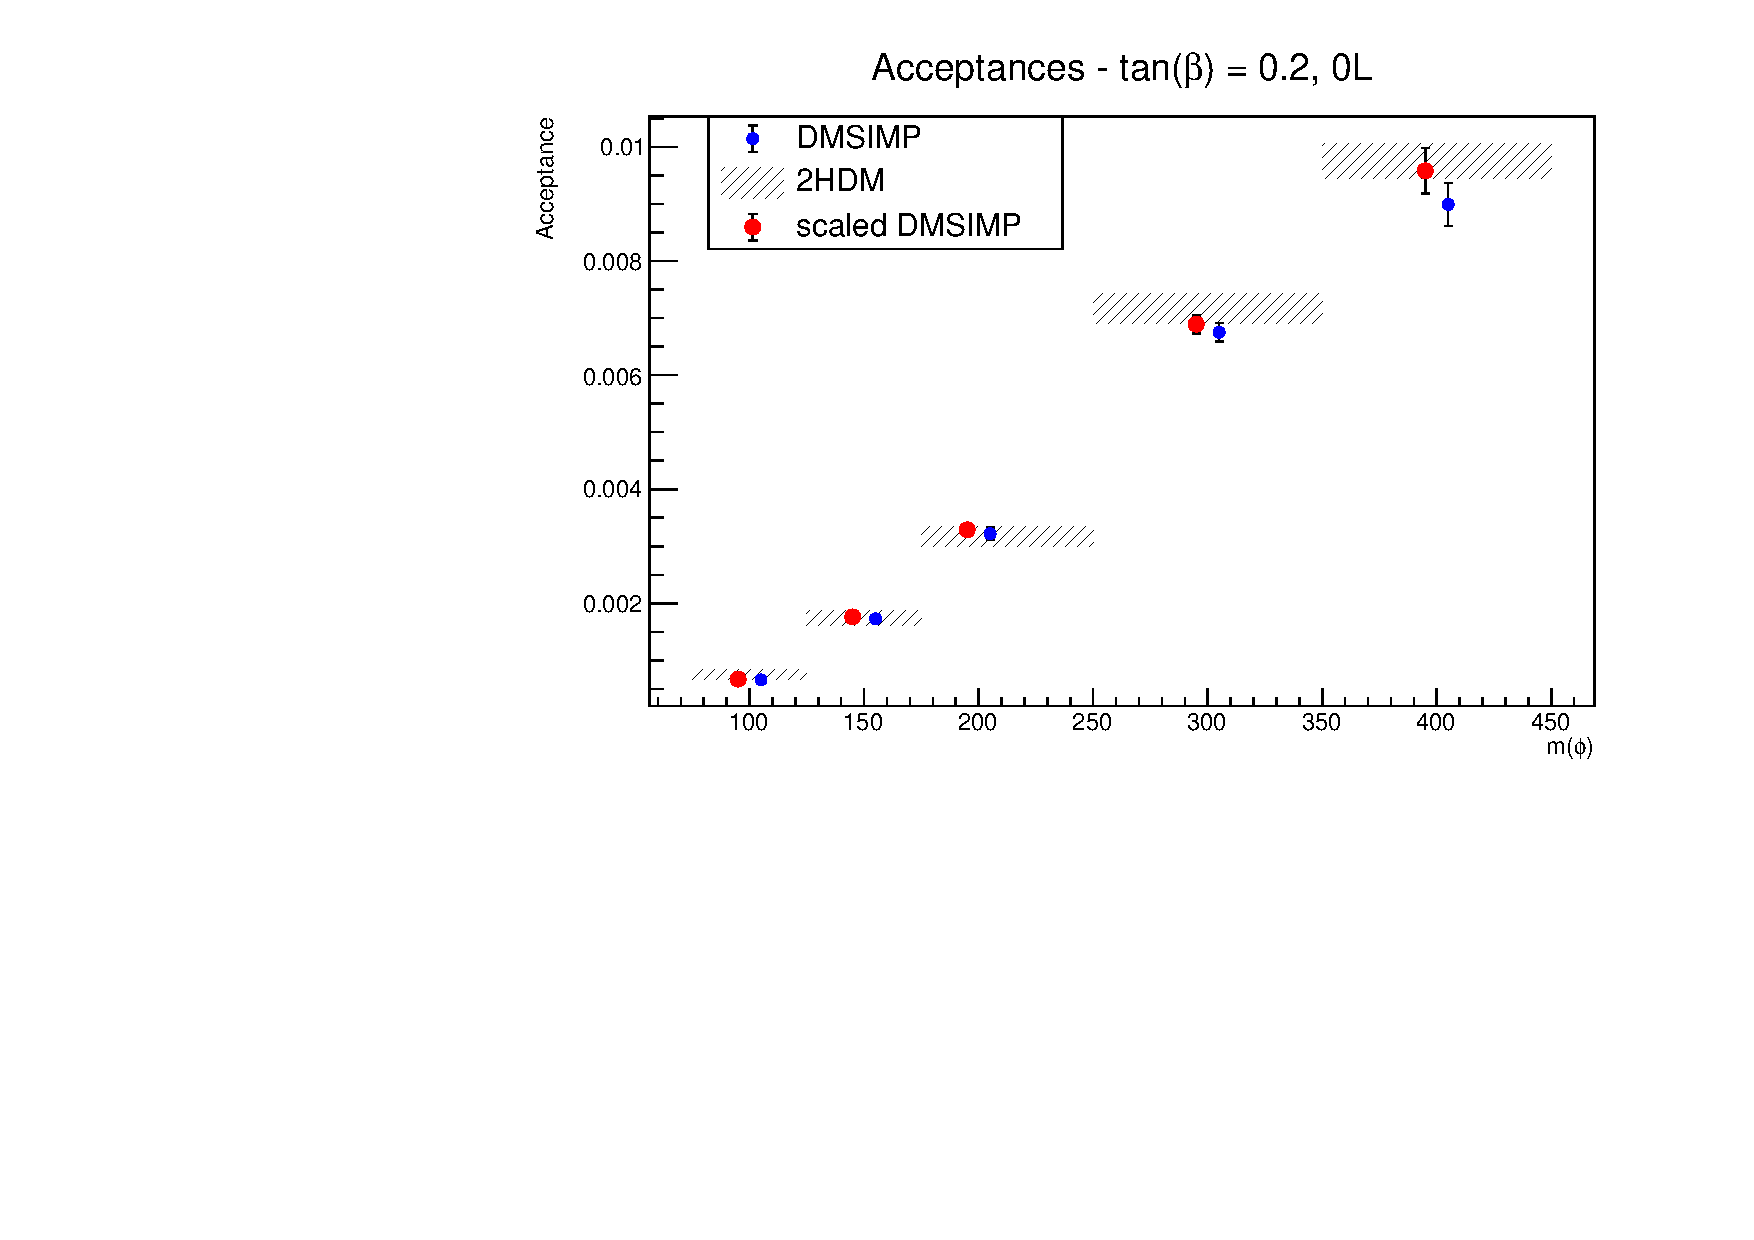
\includegraphics[width=0.6\textwidth]{texinputs/04_grid/figures/DMHF/THDMs/rescalingS1tgb02.pdf}
   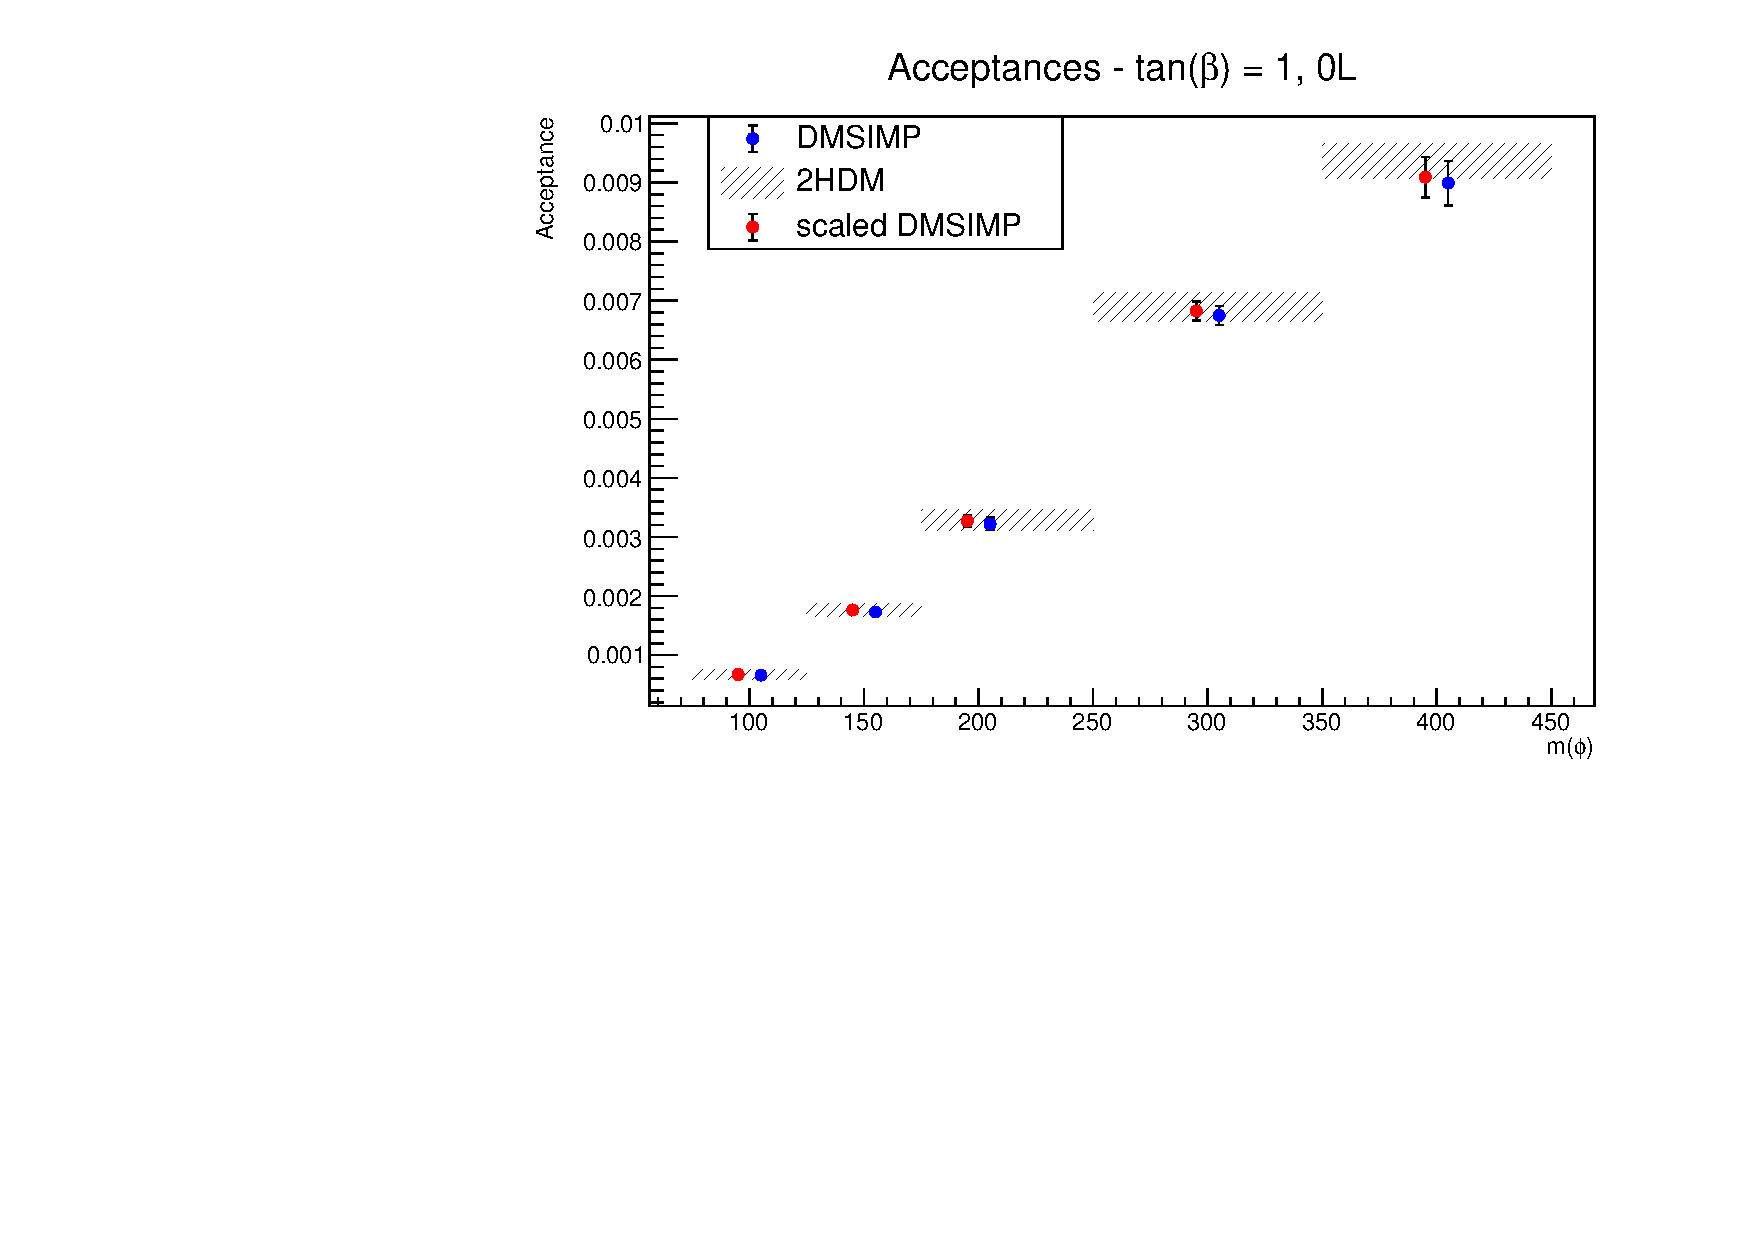
\includegraphics[width=0.6\textwidth]{texinputs/04_grid/figures/DMHF/THDMs/rescalingS1tgb10.pdf}
\caption{Validation of the re-scaling formula as a function of $m(S_1)$ for the minimum and maximum values of $\tan{\beta}$ considered.}
 \label{fig:rescS1}
\end{figure}

Fig.~\ref{fig:resultsS1} shows the results of the recasting of the simplified model results in the context of the 
$2HDM+S_1$ model. For the choice of parameters made, models with scalar mediator between 100 and 360 GeV 
can be excluded for $\tan\beta = 0.2$, while for $\tan\beta = 1$ masses between 100 and 120 GeV are excluded.

\begin{figure}
  \centering
  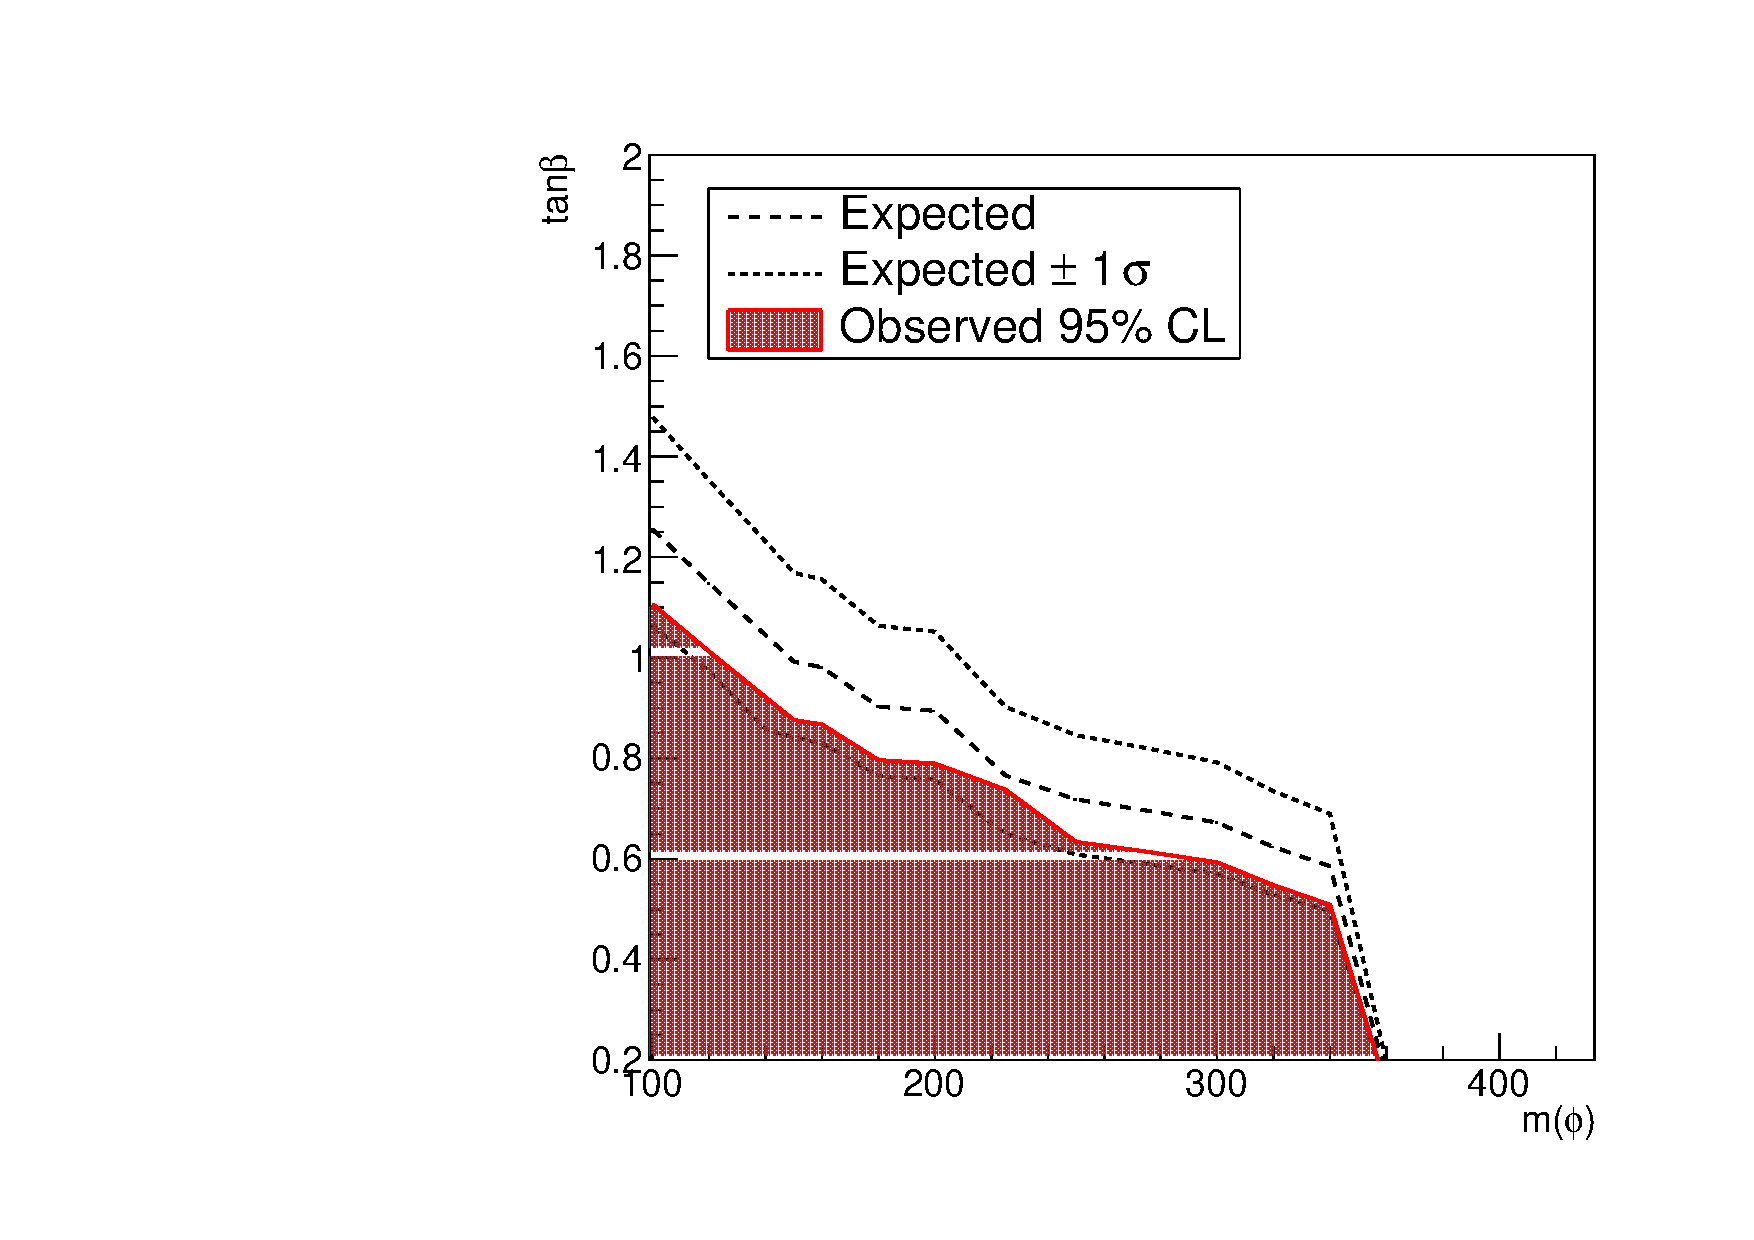
\includegraphics[width=0.6\textwidth]{texinputs/04_grid/figures/DMHF/THDMs/resultsS1.pdf}
\caption{Expected and observed exclusion limits at $95\%$ C.L. obtained as a result of the recasting of the all-hadronic channel
in the context of the $2HDM+S_1$ model.}
  \label{fig:resultsS1}
\end{figure}

%\printbibliography


%\end{document}



